\emergencystretch=1em

This work integrates a detailed interrogation of host\hyp{}pathogen interactions in the specific context of C\hyp{}type lectin signaling responses and angiogenesis. In this section, I will introduce the major concepts needed to interpret the data\hyp{}driven findings in later chapters. These topics will include: the disease itself, the fundamental biology of macrophages, the principles of C\hyp{}type lectin signaling, the NFAT signaling pathway, and angiogenesis. Each section will incorporate historical background, foundational findings in the field of interest, and contextualization for how this information educates later approaches and experimental decisions.

\section{Tuberculosis}\label{tuberculosis}

Of all the infectious agents to have ever afflicted humankind, \textit{Mycobacterium tuberculosis} is perhaps the most imminently successful \citep{Barberis2017}. The primary cause of potentially greater than one billion human deaths since 1800 alone \citep{Murray2004, Paulson2013}, ``the White Plague''\footnote{This nickname is in juxtaposition to the Black Plague, the historical disease caused by \textit{Yersinia pestis}, which decimated much of the global human population in the 1300s \citep{Perry1997}.} has had profound impact on the cultural and political development of the modern world and continues to impact the lives of most people around the world today\footnote{For additional reading on this subject of how tuberculosis has impacted the development of human society, see \citep{Chalke1962, Dubos1987, Day2017}.}, with a disproportionate impact on those who live in economically developing countries. Fallaciously considered a disease of antiquity, this disease co\hyp{}evolved with humankind \citep{Hershkovitz2015} and today manifests in active disease in greater than 10 million people\footnote{Greater than 30 million people are at constant risk of infection by cohabiting with active tuberculosis patients \citep{Ross2021}.} each year and has killed greater than one million people per year each year since records or estimates have been available \citep{Saleem2013, WHO2022} with the case and death burden rising due to health system neglect exposed by the COVID\hyp{}19 pandemic ongoing at the time of this writing \citep{Pai2022}. 

\textit{Mycobacterium tuberculosis} has long been of basic scientific interest on account of the myriad ways in which it undermines host immune responses to establish a replicative niche within the human lung \citep{Stanley2003, Monack2004, Nguyen2009, Baxt2013, Hmama2015, Yu2019}. \textit{M. tuberculosis} infection results in the formation of caseating granulomas\footnote{The biology of these granulomas is a fascinating microcosm of developmental and cell biology which will be discussed at length in \autoref{mamaw}.} encapsulated by a complex network of immune cells within which the bacteria replicate \citep{Pagan2018}. Over evolutionary time, these bacteria have innovated novel ways of subverting nearly every host\hyp{}protective immune response while exacerbating maladaptive ones in pursuit of survival and transmission \citep{Ernst2012, Rahman2020, Guan2021, Chandra2022}. This makes the study of tuberculosis not only the study of microbiology and immunology, but a fascinating study in the basic principles of cell biology informed by evolution and ecology, interwoven with history. 

\subsection{History of Tuberculosis}\label{tbhistory}

The overwhelming prevalence of tuberculosis in the 18\textsuperscript{th} and 19\textsuperscript{th} centuries led to a profound degree of cultural salience for this disease in the daily lives of the people of those times. Responsible for the deaths of many preeminent public figures of these eras\footnote{The number of such public figures is far too great to list. From the 1840s and 1850s alone, tuberculosis was responsible for the deaths of Andrew Jackson (seventh president of the United States), Henry Clay (Secretary of State, Speaker of the House, three\hyp{}time presidential candidate for the Whig Party), John C. Calhoun (Vice President, Secretary of State), Alexis de Tocqueville (famed French observer of American culture and author of the classic of political theory, \citefield{Tocqueville1835}{title}), Henry David Thoreau (naturalist author of Walden), and Emily Bront\"{e} (author of Wuthering Heights). Additionally, it is thought that George Washington may have been afflicted with intestinal tuberculosis, explaining a lifetime of gastrointestinal troubles \citep{Chernow2010} and, in the modern day, Ringo Starr of \textit{The Beatles} fame had tuberculosis and was confined to a sanitorium for some time \citep{Starr2016}.} and approximately 25\% of all deaths by any cause \citep{CDC2016}, it became a ubiquitous dimension of the literary \textit{Zeitgeist} as well. Perhaps most famously, tuberculosis is depicted as the disease that afflicts the Lowood School in Charlotte Bront\"{e}'s \textit{Jane Eyre}, among other novels depicting the disease then known as \textit{consumption} for the way in which it leads to cachexia\footnote{To be described more extensively shortly, cachexia is a progressive wasting that results in unmitigable weight loss.}, pallor, hemoptysis\footnote{The racking cough that accompanies tuberculosis is often depicted by women on chaise lounges coughing blood into a white handkerchief; the reality, of course, is far more dire \citep{Giles1802, Bouvier1842, Robinson1858, Alexander1895}.}, and ultimately death \citep{Bronte1847, Loddenkemper2015}.

This cachexia is a defining feature of tuberculosis across the diverse organisms afflicted by it; such progressive, consumptive wasting unable to be ameliorated by improved nutrition is an unusual presentation strongly reminiscent of many cancers and rather dissimilar from most infectious diseases \citep{Silva1988, Tisdale2002, Martignoni2003, Chang2013}. Indeed, as medical understanding of diseases progressed beyond concepts of humoral imbalance\footnote{This theory of humoral imbalance was prevalent from the time of the ancient Greeks until the 1800s, when more scientific approaches to the understanding of human disease were developed \citep{Lagay2002}. This theory posited that disease arose from an imbalance of the four major humors: blood, yellow bile, black bile, and phlegm. These constituted the human corpus and their balance dictates human health. We now know, of course, that diseases generally have specific causes that are able to be diagnosed by modern medicine.}, a prevailing theory was that tuberculosis was a hereditary form of cancer due to the way it spread within families \citep{Frith2014}. The functional and consequential similarities between tuberculosis and cancer are replete and will be a theme returned to throughout this document. However, as Louis Pasteur's germ theory \citep{Smith2012} came to be more widely accepted in the same period in the Industrial Revolution as Joseph Lister's antiseptic practices \citep{ToledoPereyra2010}, it became a subject of scientific inquiry to identify the potentially infectious bases for seemingly transmissible diseases\footnote{This having the caveat that tuberculosis does not always appear to be transparently transmissible. The disease can take months to years to manifest in infected persons, leading to long time delays between putative exposure and active disease \citep{Behr2018}.}. 

Robert Koch was the first to document the tubercle bacillus as the infectious etiology of tuberculosis in 1882 \citep{Koch1882, Cambau2014}. \textit{Mycobacterium tuberculosis} proved to be a foundational instrument in the broader development of the discipline of microbiology and provided Koch with the rationale for the development of what we know as the Koch's postulates\footnote{The postulates are as follows: the organism should be present in afflicted individuals, but not in healthy individuals; the organism should be able to be grown in pure culture; inoculation of a healthy host should recapitulate the disease; the organism should be able to be harvested back from the new host. Of course, each and every one of these postulates have been broken in pursuit of identifying disease\hyp{}causing agents, but this remains the basis of identifying new infectious etiologies \citep{Segre2013}.}\footnote{There is a parallel set of postulates known as the molecular Koch's postulates which are used to define the contribution of a particular gene to the virulence of a pathogen, which can be used to systematically and functionally dissect the genetic underpinnings of pathogenesis. These postulates, first proposed by Stanley Falkow are a functional adaptation of the original postulates for the molecular era \citep{Falkow1988, Falkow2004}.}, a procedural set of criteria for determining the infectious etiology of any disease. This, along with the identification of the anthrax bacillus (\textit{Bacillus anthracis}), sparked the beginning of the modern era of microbiology \citep{Koch1876}. It was only once the causative agent of tuberculosis had been identified that it became possible to earnestly pursue curative therapies and vaccines\footnote{This is an activity that Koch himself pursued, to some controversy. He publicly promised a vaccine made of homogenized bacilli; while this application failed, it provided the foundation of the tuberculin now used in the diagnostic skin test taken by millions of Americans annually \citep{Goetz2014}.}, which came swiftly thereafter to varying degrees of efficacy. By 1921, Albert Calmette and Camille Gu\'{e}rin had attenuated the closely related and conspecific \textit{Mycobacterium bovis} for use as a vaccine, creating the BCG live attenuated vaccine still in use today\footnote{The BCG vaccine is annually given to millions of newborns around the world to prevent tuberculosis, but demonstrates, at best, variable efficacy \citep{Rodrigues1993, Andersen2005, Schrager2020, Trauer2021} and a short period of protection against tuberculosis, despite inducing a lifetime's worth of immunomodulation and protection from lung cancer and all\hyp{}cause death \citep{Higgins2016}.} \citep{Hawgood2007}. 

Once thought to have been functionally banished to the annals of history, tuberculosis, after a steady decline in cases throughout the middle of the 20\textsuperscript{th} century\footnote{This was coincident with, but likely unrelated to, the development of effective antibiotic therapies. Indeed, the modern disparity between tuberculosis rates between the United States and Western Europe and much of the rest of the world is thought to have more to do with improved living conditions, growing herd immunity, and improved nutrition rather than the use of antibiotics as downward trends actually began 100 years prior to the discovery of streptomycin in 1944 \citep{Lowbury1958}.}, came roaring back later in the century with the introduction of HIV into the human population in the 1980s. HIV/AIDS causes an immunodeficiency that increases susceptibility to infection, disease, and death from tuberculosis, which has become an AIDS\hyp{}defining illness \citep{Selwyn1992, Drobniewski1995}. Compounding these troubles, particular strains of \textit{M. tuberculosis} have developed resistance to many of the commonly used antibiotic therapies available, leading to the emergence of multi\hyp{}drug resistant strains that increase cost of treatment, acute patient burden, and duration of therapy \citep{Matteelli2014}.

\subsection[The Pathogenic Lifestyle of \textit{Mycobacterium tuberculosis}]{The Pathogenic Lifestyle of \textit{Mycobacterium tuberculosis}\footnote{For excellent reviews on this topic, see \fullcite{Philips2012} and \fullcite{OGarra2013}.}}\label{path:tb}

The study of \textit{M. tuberculosis} has long focused on factors that drive its virulence; that is, its ability to cause disease, evade immune responses, overcome antibiotic therapy, and transmit to new hosts \citep{Glickman2001b}. These studies have revealed innumerable ways by which this pathogen accomplishes these tasks and many potential targets for new antitubercular therapies both via bacterial factors and host\hyp{}protective and \hyp{}detrimental immune responses. In many regards, the study of tuberculosis is the study of so\hyp{}called ``anti\hyp{}immunology'' given the vast spectrum of mechanisms used to undermine the host and the frequent failure of the host to mount a sufficient immune response \citep{Finlay2006, Diacovich2010}.

In addition to the clear relevance of the study of tuberculosis to human health, the unique biological features of this acid\hyp{}fast, genetically\hyp{}insular\footnote{Some, but not all \textit{Mycobacterium} spp. can undergo horizontal gene transfer, but the mechanisms are poorly understood. Indeed, the challenge of shuttling DNA across the cell wall was a major impediment in the development of genetic tools to study mycobacterial genetics in the lab. However, \textit{M. tuberculosis} \textit{sensu stricto} is not thought to be competent for natural gene transfer \citep{Krzywinska2004, Galagan2014, Derbyshire2014, Reva2015, Merker2015, Boritsch2016, Madacki2021}.}, non\hyp{}motile, slow\hyp{}growing\footnote{\textit{M. tuberculosis} doubles approximately once every 24 hours, compared to \textit{Escherichia coli} which can double once every 20 minutes in log\hyp{}phase.} mycobacterial species make it a fertile ground for basic scientific studies into the way that both saprophytic and pathogenic species of bacteria adapt to adverse environments and ultimately establish a productive niche \citep{Pieters2002, Houben2006, Falkinham2009, Prasanthi2014, Ghodbane2014, Delafont2014}. The physiological features of the bacillus -- a thick, hydrophobic cell wall \citep{Jarlier1994, Chatterjee1997, Jankute2015}, unique export and import systems \citep{Braibant2000, Pandey2008, Tullius2011, Houben2014, Wong2017a, Palmer2017, Famelis2019, Bunduc2020}, and novel mechanisms for cell division \citep{Dziadek2003, Hett2008, Kieser2014, Odermatt2020} and stress tolerance \citep{Garg2015, Peddireddy2017} -- make this a fascinating case study in the evolutionary processes that drive niche adaptation and, indeed, niche creation \citep{Chapman1971, Warner2007, deChastellier2009, Gengenbacher2012, Lerner2016, Honda2018, Gagneux2018, Sarathy2020, Pereira2020, Lovewell2021}. 

That related members of the same genus of bacteria occupy such diverse infectious niches across a wide spectrum of organisms (from fish and amphibians and reptiles to birds and mammals and in every major organ system), with many also possessing stages of growth in the environment is a testament to the extent to which these species have evolved structures and responses that can accommodate a wide range of physical and chemical stressors \citep{Thoen1981, Palmer2011, Hershberg2016, Saelens2019, Larsen2020}. By contrast, some species, notably \textit{M. tuberculosis} and \textit{M. leprae}\footnote{Leprosy, the classical Biblical affliction, is another prominent human disease caused by a mycobacteria. The biology of leprosy is fascinating and will be touched on sporadically throughout this dissertation \citep{Schamberg1899}.}, are tightly adapted to a more limited range of hosts and are thought to have lost the capacity for long\hyp{}term survival outside of a mammalian host, although this is now under some contention with the identification of infection\hyp{}competent \textit{M. tuberculosis} from soil samples \citep{Martinez2019, Ploemacher2020, Borham2022, Mtetwa2022}. This diversity within the genus offers abundant opportunity for gene\hyp{}structure\hyp{}function discovery to uncover factors both required for maintaining an environmental niche as well as those specifically required for either commensal or pathogenic association with the host, an approach that has long been fruitful in the discovery of novel virulence factors \citep{Sassetti2003, Ehrt2015} but comparatively neglected in the basic bacteriological study of environmental mycobacteria.

When a pathogenic \textit{Mycobacterium} infects a na\"{i}ve host, an intricate set of cellular and signaling responses occur at the interface of the host and the bacterium that facilitate either successful clearance or establishment of a productive infection \citep{Davies2001b, Gagneux2006a, Turner2017, Bohrer2021}. The summative effect of these immune responses determines the outcome of the infection and careful balancing on the part of the host must take place to both kill the pathogen and minimize host pathology \citep{Casadevall1999, Casadevall2003}. Taking human tuberculosis infection as the model, productive infection will result in patients coughing aerosolized droplets that often contain a single bacillus \citep{Churchyard2017, Mathema2017}. These individual bacilli can then be inhaled by a na\"{i}ve person nearby, establishing a new cycle of infection. Once that person has inhaled this bacterium\footnote{Unlike many other diseases, increasing the infectious inoculum paradoxically reduces the risk of disease -- large clumps of bacteria are unable to reach the distal lung where they are better able to establish infection \citep{Cambier2014b}.}, lung\hyp{}resident macrophages\footnote{Also known as alveolar macrophages, these are one of many, many different types of tissue\hyp{}resident macrophages. While it is well beyond the scope of this section to explore fine distinctions, but suffice it to say that macrophages in each tissue niche are functionally distinct from one another and exhibit distinct responses to stimuli. Tissue\hyp{}resident macrophages are also established from a non\hyp{}hematopoietic origin from the fetal yolk and are replication\hyp{}competent, allowing them to self\hyp{}renew \textit{in situ} \citep{Davies2013a, Davies2013b, Epelman2014, Ginhoux2014, Ginhoux2016}. The study of macrophage biology is one of immense challenge and opportunity to uncover novel roles for these multifunctional cells, which are now known to play important roles in processes as diverse as germ cell maturation, metabolism, sleep, cardiovascular disease, and many more \citep{Davies2013a, Hussell2014}. Some of these will be addressed in greater detail in \autoref{macrophages}.} phagocytose the bacteria. In many instances (approximately 90\% of the time), the macrophage will successfully kill the bacteria, but in the other 10\%, the bacteria are able to survive, replicate, and progress to either latent or active disease \citep{North2004, Verrall2014, Pai2016, Kroidl2022}.

If initial clearance or containment fails, a complex cascade of events proceeds. After phagocytosis, the macrophage sets in motion signaling processes that should result in fusion between the phagosome and extant lysosomes within the cytosol \citep{Abramovitch2011}. However, the bacteria, through a combination of structural features in the cell wall (more on this in \autoref{tdm}) and secreted effector proteins, blocks phagosomal\hyp{}lysosomal fusion to establish a replicative niche in the macrophage within a parasitophorous vacuole \citep{McDonough1993, Pieters2008, Casonato2014}. Subsequently, the outpouring of secreted effectors from the bacteria across the phagosomal membrane into the host cytosol results in profound reprogramming that blocks apoptosis \citep{Keane1997, Keane2000, Yokobori2012, Maueroder2016, Ahluwalia2017, Beckham2017, Wong2017a}, downregulates production of select cytokines and chemokines (while enhancing the expression of others) \citep{Fortune2004, MadanLala2011, Cambier2014a}, directs the macrophage to recruit additional macrophages to further the replicative cycle \citep{Cambier2014b, Appelberg2015, Pagan2015}, and guides the macrophage out of the lung proper and into the interstitial space surrounding the lungs, the actual site of primary infection \citep{Peters2003, Ramakrishnan2012, Upadhyay2018, Cohen2018}. Due to the slow growth of \textit{M. tuberculosis}, it can take several days before the macrophage has become filled with such a large number of bacteria that it necroses\footnote{There is some interesting biology behind this, where \textit{M. tuberculosis} actively inhibits apoptosis to allow itself to grow to high burden within the macrophage and then lyse it to be released into the extracellular milieu \citep{Keane2000}.}, allowing the bystander macrophages and neutrophils to be infected anew \citep{BanosMateos2017}. This cycle continues as more immune cells are recruited by the escalating infection and more extracellular bacteria accumulate \citep{Lin2006a, Orme2014a, Cadena2016, Corleis2020}. These stages of infection, cell lysis, aggregation, and further recruitment eventually result in the formation of what we know as a granuloma \citep{Ramakrishnan2012, Pagan2018}. 

Tuberculous granulomas are complex aggregates of (primarily) macrophages that have differentiated into a less inflammatory\footnote{Some might say M2\hyp{}like state, but the M1\hyp{}M2 binary axis is, rightfully, under attack in the era of single cell \hyp{}omics. This false dichotomy neglects the full spectrum of activation states possible for macrophages and the plasticity with which a given macrophage can change it's activation state based on the particular set of signals being received at a granular point in time \citep{Martinez2014, Ley2017}. See also \autoref{lies}.}, epithelioid state that encapsulate a central focus of extracellular bacteria within a necrotic core \citep{Boros2003, Rubin2009, Cronan2016}. These epithelioid macrophages are augmented by the full spectrum of other immune cell types -- inflammatory macrophages, neutrophils, basophils, eosinophils, natural killer cells, T cells, B cells, and a range of stromal cells \citep{Russell2007, Ramakrishnan2012}. As a discrete structure, these provide a full immunological nexus integrating essentially every identifiable immune cell population and may provide a pathology\hyp{}minimizing approach to infection containment despite relative costs and benefits that will be explored more so later on \citep{Casadevall2003}. They also display a great deal of heterogeneity from granuloma to granuloma and person to person, reflecting key variations in the immune and bacterial responses over time \citep{Cadena2017, Gideon2022}. These granulomas, although extractable intact from their environment, must exist in a tissue environment not of their own immediate design \citep{Kaplan2003, Datta2015, Cronan2018, McCaffrey2022}. These microenvironmental factors, while of long\hyp{}standing interest in tumor biology, have yet to be properly explored in the context of tuberculous granulomas. Although immune cells can be readily recruited, the extrapulmonary space is a pre\hyp{}existing physical location that can be remodeled to some degree but is inherent in the course of the infection. Mycobacteria are tasked with manipulating these tissues, which they do not directly infect\footnote{This is not true \textit{sensu stricto} as \citet{Cohen2018} observed transient infection of pulmonary epithelial cells, but this fades within a few days -- the consequences of these infections are not known. Lasting memory of these events may influence outcomes of other infections or superinfecting mycobacteria, similar to findings in influenza viruses, which leave behind a pool of surviving epithelial cells after infection \citep{Heaton2014, Hamilton2016, Dumm2019, Fiege2019, Dumm2020}.}, to further their own lifestyle. One of the ways they do this, and which is the focus of much of this work, is by inducing the pathological growth of blood vessels toward the site of infection in a process known as angiogenesis.

The clinical description of hemoptysis is a clear manifestation of this vascular involvement in the disease \citep{Souders1952, Middleton1977, Turner2003a, Turner2003b}. As the granuloma cavitates and releases its contents into the airway, the encapsulating vasculature is destroyed. While such damage could have occurred incidentally by damaging the vessels that service the alveoli, it is now clear that much of this hemorrhage is the product of the encapsulating vascular web that develops around the granuloma over the course of the infection \citep{Cudkowicz1952, Oehlers2015, Datta2015}. These clinical observations have, however, left unaddressed the role for this vasculature in the development, progression, transmission, and treatment of the disease. The former two questions are the subject of the present work while the latter two remain promising avenues of future discovery.

\subsection{Treatments for Tuberculosis and their Mechanisms of Action}\label{treatments}

Mycobacterial infections are uniquely integrative biological phenomena that require a delicate balance between the host and the pathogen. The host, in order to eradicate the bacteria, seeks a potent but highly specific sterilizing immune response while the bacteria, seeking to establish a replicative niche, must evade these host defenses. Both must avoid inducing excessive tissue damage, which may reduce the fitness of both organisms -- the host through impaired survival and reproduction and the pathogen by early termination of a route of transmission. Chemotherapeutic treatment of infection seeks to tip the scales back in favor of the host by targeting processes essential for bacterial survival. Historically, treatment for bacterial infections has been through the application of these bacteria\hyp{}targeting antibiotics\footnote{The most classic example is penicillin, which was discovered in 1941 by Alexander Fleming and sparked a revolution in the treatment of countless battlefield diseases during World War II, saving countless lives \citep{Fleming1941, Henderson1997}. While many bacteria have developed resistance to penicillin through expression of penicillin\hyp{}binding proteins or beta\hyp{}lactamase, other antibiotics have filled in some of these gaps to treat these resistant strains \citep{Eagle1954, Sabath1977, Murray1983, Klare1992}.}, despite their mechanism of action rarely being understood at the time of clinical introduction \citep{Osborne2013, DAmbrosio2015}. Modern tuberculosis infections are treated with a four\hyp{}drug cocktail of antibiotics over the course of six to nine months: isoniazid, ethambutol, pyrazinamide, and rifampin \citep{Grace2019, Dorman2021}. Should the bacteria exhibit resistance to one or more of these, a state known as multi\hyp{} or extensive\hyp{}drug resistance (MDR/XDR), additional drugs with further host toxicity are used: kanamycin, ciprofloxacin, and cycloserine are common choices, although new drugs are slowly coming onto the market \citep{Quenard2017, Nahid2019, Jang2020}. Of these, bedaquiline appears to have the most promise in improving the overall treatment of tuberculosis, but long\hyp{}term impact remains to be seen \citep{Mahajan2013, Pym2016, Furin2017}. 

The first modern, clinically effective treatment for tuberculosis was pioneered by the discovery of streptomycin from \textit{Streptomyces griseus} in 1943 \citep{Hinshaw1946, Hinshaw1947, Comroe1978}. Unlike its antibiotic predecessor, penicillin, streptomycin was effective in killing \textit{Mycobacterium tuberculosis} bacilli \textit{in vitro}. However, due to its lack of oral bioavailability, the use of this drug was limited to hospitals and clinics able to deliver the drug intravenously. Additionally, like many of the attempts at drug development for tuberculosis that had preceded it\footnote{One of these, para\hyp{}aminosalicylic acid (PAS) is an interesting, if distracting tale in the history of microbiology. For more information, see \citep{Dubovsky1988, Donald2015}}, it was not particularly effective at eliminating disease when used alone and resistance quickly emerged \citep{Pfuetze1949, Ruiz2003}. Streptomycin is an aminoglycoside antibiotic that interferes with protein biosynthesis by poisoning the 30S subunit of the ribosome \citep{Sharma2007}. This mechanism is common to all of the diverse bacteria against which streptomycin is effective, making it a good general purpose antibiotic, if somewhat limited in the face of the unique features of mycobacterial anatomy.

Thus, the introduction of a mycobacteria\hyp{}specific antibiotic in the form of isoniazid in 1952 was a major breakthrough in the treatment of this disease \citep{Goldman1972}. Orally bioavailable and highly effective at killing mycobacteria, it comes with the dose limiting side effects of peripheral neuropathy and occasionally fatal hepatitis that make it a less than perfect therapeutic option \citep{Maddrey1973, Black1975, Metushi2011, Metushi2016, Diallo2018}. Nevertheless, it is still in use today on account of its synergy with other antimycobacterials and independent efficacy. Isoniazid works by targeting mycobacterial cell wall synthesis via InhA inhibition to block earlier stages of fatty acid biosynthesis \citep{Timmins2006, Vilcheze2007}. This prevents the synthesis of the mycolic acids that comprise the outermost layer of the cell wall and which are essential for mycobacterial survival, growth, and immune evasion \citep{Rozwarski1998, Lei2000, Vilcheze2006, Timmins2006}. 

Recognizing the inherent limitations of isoniazid monotherapy, additional drugs came into use over the next twenty years. Next on the list of drugs was ethambutol, which entered into use in 1961 \citep{Thomas1961, Chakraborty2015}. Ethambutol, like isoniazid, targets the synthesis of the cell wall, this time by inhibiting the enzymatic ligation of arabinogalactan, which bridges the lower peptidoglycan layer and the outer mycolic acid layer, destabilizing the cell wall and increasing bacterial susceptibility to immune killing \citep{Safi2013, Zhang2020a}. Interestingly, the precise mechanism of action of ethambutol remains unknown despite over 60 years of extensive study, although cross resistance with isoniazid is common, suggesting some overlapping target pathways \citep{Gupta2006, Zhang2020a}.

Rifampin (1965) was the next addition and has an entirely distinct mechanism of action compared to the previous entrants. Targeting multiple, simultaneous, essential biological pathways is an excellent and repeatedly proven way of killing pathogens and preventing the emergence of resistance to all of the drugs simultaneously as such coordinate genetic mutation is exceedingly unlikely and even more so given the slow mutation rate of \textit{Mycobacterium} species\footnote{At a rate of approximately two base pair changes per 10,000 replications, it can take weeks or months for this slow growing bacteria to happen upon a resistance\hyp{}conferring mutation \citep{McGrath2014}.} \citep{Pletz2017}. Rifampin targets RpoB, the major subunit of the bacterial DNA\hyp{}dependent RNA polymerase, which is essential for transcription \citep{Wehrli1983, Telenti1993}. Although mutations have arisen that confer resistance to rifampin, these have particular fitness costs on the bacteria under conditions lacking antibiotic pressure \citep{Billington1999, Mariam2004, Gagneux2006b, Gagneux2009, Xu2021a}. Rifampin has proven to be an excellent antimycobacterial drug with a comparatively favorable side effect profile compared to the other commonly used drugs and is universally used for treatment of both latent and active tuberculosis\footnote{Rifampin treatment is the origin of the oft\hyp{}repeated but foundationally untrue warning given to women on hormonal contraceptives to beware antibiotics. While rifampin has been shown to reduce blood estrogen concentrations, there is no evidence of other drugs having these effects. Common antibiotics are vanishingly unlikely to interfere with oral contraceptives and these warning labels are both unnecessary and misleading \citep{Skolnick1976, Zhanel1999, BarditchCrovo1999, Archer2002, Simmons2018a, Simmons2018b}.}.

To round out the four drug cocktail generally recommended for the first\hyp{}line treatment of tuberculosis today, pyrazinamide (1972) is the most mechanistically interesting of this antibiotic panel \citep{Yeager1952, Steele1988, Millard2019}. It appears to work by diffusion into the acidic necrotic center of the granuloma where protons activate the prodrug by nucleophilic attack of the amide bond, allowing it to be enzymatically converted by the bacteria into pyrazinoic acid, the active antimicrobial \citep{Kalinda2012, Zhang2013, Zhang2019, Lamont2019, Villagracia2020, Lamont2020}. The low pH maintains the stoichiometry in favor of the protonated pyrazinoic acid form over the conjugate base pyrazinoate, facilitating diffusion into the cytosol of the bacteria across the hydrophobic cell membrane. Despite the knowledge that has been ascertained about the precise conditions under which pyrazinamide is active, the mechanism of action remains under hot contention with a variety of different mechanisms proposed and the most recent -- that it inhibits the synthesis of the essential fatty acid and metabolic carrier coenzyme A -- still under dispute as the mechanism of resistance is typically through mutations in \textit{pncA}, the pyrazinamidase \citep{Zhang2003, Shi2011, Kalinda2012, Zhang2014a, Dillon2017, Lamont2020}. Pyrazinamide, entirely by accident, takes advantage of the particular biological environment of the infecting bacteria to specifically target the pathogen. As a relatively innocuous prodrug that is activated at the precise site of infection, it is able to ameliorate some of the toxic effects that would be associated with direct use of pyrazinoic acid while concentrating active drug where bacteria are actively growing with passive diffusion moving additional prodrug into the granuloma to be activated and trapped inside the necrotic caseum \citep{Wade2004, Gopal2016}. Replicating such effects with other prodrugs seems like an effective means of improving safety and efficacy profiles, although the rational design of such drugs is certainly far from trivial.

Modern antibiotic development generally has been stymied by a lack of incentive for the expenditure of research and development funding on costly, low profit drugs \citep{Joshi2011}. As new antibiotics are likely to be reserved for cases with extensive antibiotic resistance and are likely to be cost\hyp{}prohibitive for broad use, few have been developed despite pressing need. One of the success stories is that of bedaquiline, which was first approved in 2012 and represents an entirely new class of antibiotics. The development of bedaquiline required ~\$500 million in public investment compared to ~\$100 million in investment by the profiteering corporation, Janssen Biotech \citep{Osborne2013, Leibert2014, Gotham2020}. Bedaquiline is a potent and highly effective drug reserved for use in multidrug resistant (MDR) and extensively drug resistant (XDR) cases of tuberculosis and which acts to block ATP synthase to shut down bacterial metabolism and directly leads to bacterial death \citep{Nguyen2018, Sarathy2019}. 

\subsection{The Mycobacterial Cell Wall}\label{cellwall}

Given that inhibition of cell wall biosynthesis is a common and highly effective mechanism of action for many antimycobacterial drugs\footnote{Isoniazid, ethambutol, ethionamide, pyrazinamide (indirectly), cycloserine, and vancomycin, among others \citep{Nataraj2015}.}, this structure is of clear importance to the survival and pathogenic success of these bacteria. \textit{In vitro}, mycobacteria are unique microbes that grow in intricate serpentine cords along agar plates \citep{Koch1882, Glickman2000}. These cords were among the first observations that helped to classify diverse mycobacterial species together and defining the ontogeny of these cords was of immense concern to early mycobacteriologists. By the 1950s these scientists had identified what they called the cord factor -- a discrete molecule required for the cording effect seen in mycobacteria and that is, indeed, able to replicate key features of cording in isolation, even in the absence of bacteria, demonstrating that cording is a biophysical property of this underlying factor \citep{Sorkin1952, Bloch1953, Bloch1955, Behling1993, Hunter2006a}. This cording phenotype can play important roles during infection, where cords are difficult or impossible for macrophages to phagocytose and allow for immune evasion \citep{Bernut2014, Ufimtseva2018}. 

The chemical composition of this cord factor was soon determined and this allowed it to be given a name -- trehalose 6\hyp{}6'\hyp{}dimycolate or TDM \citep{Noll1956a}. TDM features a trehalose head group and two long mycolate tails that can extend up to C\textsubscript{100} in length, creating an incorrigibly hydrophobic molecule that forms a thick amphipathic bilayer at the surface of the mycobacteria with the trehalose moieties facing the outside world and attached to the arabinogalactan layer below with a dimensionally thick\footnote{Up to 40 nm in thickness.} interior of interleaved mycolic acid chains \citep{Glickman2008, Welsh2013, BansalMutalik2014, Alderwick2015, Adhyapak2020, Batt2020}. TDM is the predominant mycolic acid species in this cell wall layer\footnote{40\% of the total dry mass of mycobacteria is comprised of lipids, making these a critical part of the lifestyle of mycobacteria and exceptional among other bacterial genera \citep{Jackson2014}.} and has been studied since its discovery for the ways in which it contributes to mycobacterial fitness in a diverse range of environments, including and especially the human host with even the earliest observations noting its toxicity \citep{Bloch1953, Noll1956b}.

The bacterial surface is encapsulated by concentric layers of distinct biomolecules that serve distinct structural and immunomodulatory functions \citep{Neyrolles2011}. Peptidoglycan is a ubiquitous feature of bacteria and the roles of peptidoglycan in modulating host immune responses have been reviewed extensively elsewhere \citep{Kang1998a, Guan2007, Wolf2018}. Beyond and interspersed with the peptidoglycan cell wall, arabinogalactans serve as critical supports for the outer mycomembrane. However, these arabinogalactans also serve important immunomodulatory functions in yet another demonstration of the economizing nature of mycobacterial host subversion. For instance, lipoglycans can be detected by TLR2 and stimulate host inflammatory responses important for macrophage recruitment and granuloma formation \citep{Gilleron2006}.

In addition to TDM, the cell wall or outer membrane contains many other biologically active compounds that play important roles in both bacterial homeostasis and host\hyp{}pathogen interactions \citep{Yu2012, Alderwick2015, Rens2021}. One of these, phthiocerol dimycoceroserate (PDIM) appears to play a specific role in mycobacterial growth in the lung but not in other organs, perhaps implying a role for this lipid in adaptation to the primary site of infection in modern human tuberculosis \citep{Cox1999}. This molecule is able to mask underlying immunostimulatory molecules from detection by the host immune system; in the absence of PDIM, TLR\hyp{}dependent recruitment of macrophages enhances bacterial clearance \citep{Cambier2014b, Day2014}. It has also been suggested that PDIM facilitates mycobacterial escape from the phagosome of both host macrophages and lymphatic endothelial cells and, eventually, release into the extracellular space \citep{Quigley2017, Lerner2018}. Finally, in an entirely novel mechanism of action, PDIM dissociates from the \textit{Mycobacterium} and integrates into the host cell membranes, where it suppresses immune activation; this depends on host cholesterol, providing an opportunity for host\hyp{}directed intervention to overcome PDIM\hyp{}dependent immunomodulation via use of widely prescribed statins \citep{Stancu2001, Cambier2020}.

A second class of modulatory lipids are the phenolic glycolipids (PGLs). PGL has been found to be essential for the bacterial transition from survival within tissue\hyp{}resident macrophages, which have some microbicidal activity, into patrolling monocytes, which are thought to be even more permissive for bacterial growth \citep{Sinsimer2008, Barnes2017}. PGL stimulates the tissue\hyp{}resident macrophages to produce CCL2, a monocyte\hyp{}attractive chemokine, which enables the transfer of the bacteria into a more permissive growth environment. Acute blockade of CCL2 signaling improved bacterial killing by trapping them within the tissue\hyp{}resident macrophages \citep{Cambier2014b, Cambier2017}. In leprosy, PGL has been found to stimulate macrophages to produce reactive nitrogen species that are able to damage nerve fibers, a major contributor to the demyelination effect seen in leprosy \citep{Madigan2017}. In tuberculosis, these reactive nitrogen species are thought to act as a microbicial mechanism, but these radical species can also act to damage host tissues as well \citep{Ohno2003, Voskuil2011, Idh2017}. A final interesting cell wall lipid is sulfolipid\hyp{}1, which had been thought to paradoxically act to restrict bacterial growth in macrophages \citep{Gilmore2012, Seeliger2012}, but has since been identified to specifically activate nociceptive neurons in the lung to induce coughing as a means to facilitate transmission to new hosts \citep{Ruhl2020}.

Due to this complex outer membrane structure, mycobacteria do not fit into standard binary classifications of bacteria within the Gram staining system\footnote{The Gram stain utilizes a series of stains that bind to the peptidoglycan layer of Gram positive bacteria and render them visibly violet while Gram negative bacteria are counterstained magenta \citep{Bartholomew1952}.}. While Gram\hyp{}negative bacteria feature both an inner and outer phospholipid membrane, Gram\hyp{}positive bacteria have only a single plasma membrane but are encased in a thick layer of peptidoglycan \citep{Salton1953, Carlone1982}. Although evolutionarily derived from the Gram\hyp{}positive bacterial phylum \textit{Actinomycetota}\footnote{This large phylum of bacteria includes incredible diversity and a number of other important human pathogens with varying degrees of relatedness to \textit{Mycobacterium}. A notable example is \textit{Corynebacterium diphtheriae}, the causative agent of diphtheria, which also produces mycolic acids, albeit shorter in length \citep{vanderPeet2015}. The existence of a highly effective vaccine to diphtheria while no effective vaccine exists against tuberculosis is emblematic of the divergent strategies these species use to undermine their hosts \textit{C. diphtheriae} produces a classical toxin, diphtheria toxin, that is responsible for much of the pathology of disease while M. tuberculosis was thought to lack toxins until the discovery of the tuberculosis necrotizing toxin (TNT), although this is only selectively expressed and not thought to be absolutely essential for disease \citep{Danilchanka2014, Sun2015, Pajuelo2018, Tak2019, Pajuelo2020, Pajuelo2021, Tak2021, IzquierdoLafuente2021}.}, mycobacteria possess features of both Gram\hyp{}postive and Gram\hyp{}negative bacteria: they have a single phospholipid bilayer and a thick peptidoglycan layer, but also have an additional membrane comprised of mycolic acids which is occasionally referred to as the \textit{mycomembrane} \citep{Brennan1995, Chatterjee1997, Brennan2003, Jankute2015}. This mycomembrane is the defining characteristic of mycobacteria and, as we have seen, plays critical roles in the lifestyle of the bacteria. Many of these roles are exercised by a single component -- trehalose 6\hyp{}6'\hyp{}dimycolate, or TDM.

\subsection{Trehalose 6\hyp{}6'\hyp{}Dimycolate (TDM)}\label{tdm}

The mycomembrane and its primary constituent, TDM, have many well\hyp{}defined roles in providing tolerance to environmental stress, detoxifying reactive oxygen species \citep{Chan1989}, providing dehydration resistance \citep{Harland2008}, and modulating host immune responses \citep{Lima2001, Ryll2001, Harland2008, Das2013a, Asmar2016, Hunter2016, Patin2017b}. TDM, for instance, is able to block a key step in phagosomal maturation, which would normally be able to kill the bacteria after uptake into phagocytic immune cells, including macrophages and neutrophils \citep{Spargo1991, Indrigo2003, Axelrod2008}. TDM also stimulates the production of a range of cytokines by macrophages and can autonomously induce granuloma formation \citep{Korf2005}. The broad ability of TDM to mediate mycobacterial interactions with the environment is one of the critical dimensions in the evolution of mycobacteria and the ability to then utilize novel modifications on this same molecular framework to undermine host immune responses appears to have been essential for their transition to a pathogenic or commensalistic\footnote{This notion of commensal mycobacteria warrants a vast degree of additional study. Although the laboratory model of non\hyp{}pathogenic mycobacteria, \textit{Mycobacterium smegmatis}, was isolated from syphilitic chancres and, later, smegma, very little is known about the niche of these commensal mycobacteria, how they maintain a neutral or neutral\hyp{}positive relationship with their (often transient) hosts, and how their presence impacts host immunity to future encounters with pathogenic mycobacteria \citep{Robinson2018}.} lifestyle in association with eukaryotic hosts ranging from amoeba\footnote{As with many common human pathogens, it is theorized that mycobacteria developed the strategies necessary to overcome human macrophage responses on the amoebic training ground; the strategies utilized by amoeba to digest their prey are similar to those utilized by macrophages to eradicate invaders and virulence strategies that target these pathways are likely to be translatable across diverse organisms \citep{German2013, Escoll2013, Price2014, Abukhalid2021, Fu2021}.} to fish to humans \citep{Hagedorn2009, Salah2009, Falkinham2009, Delafont2014, Honda2018}.

\begin{figure}
\centering
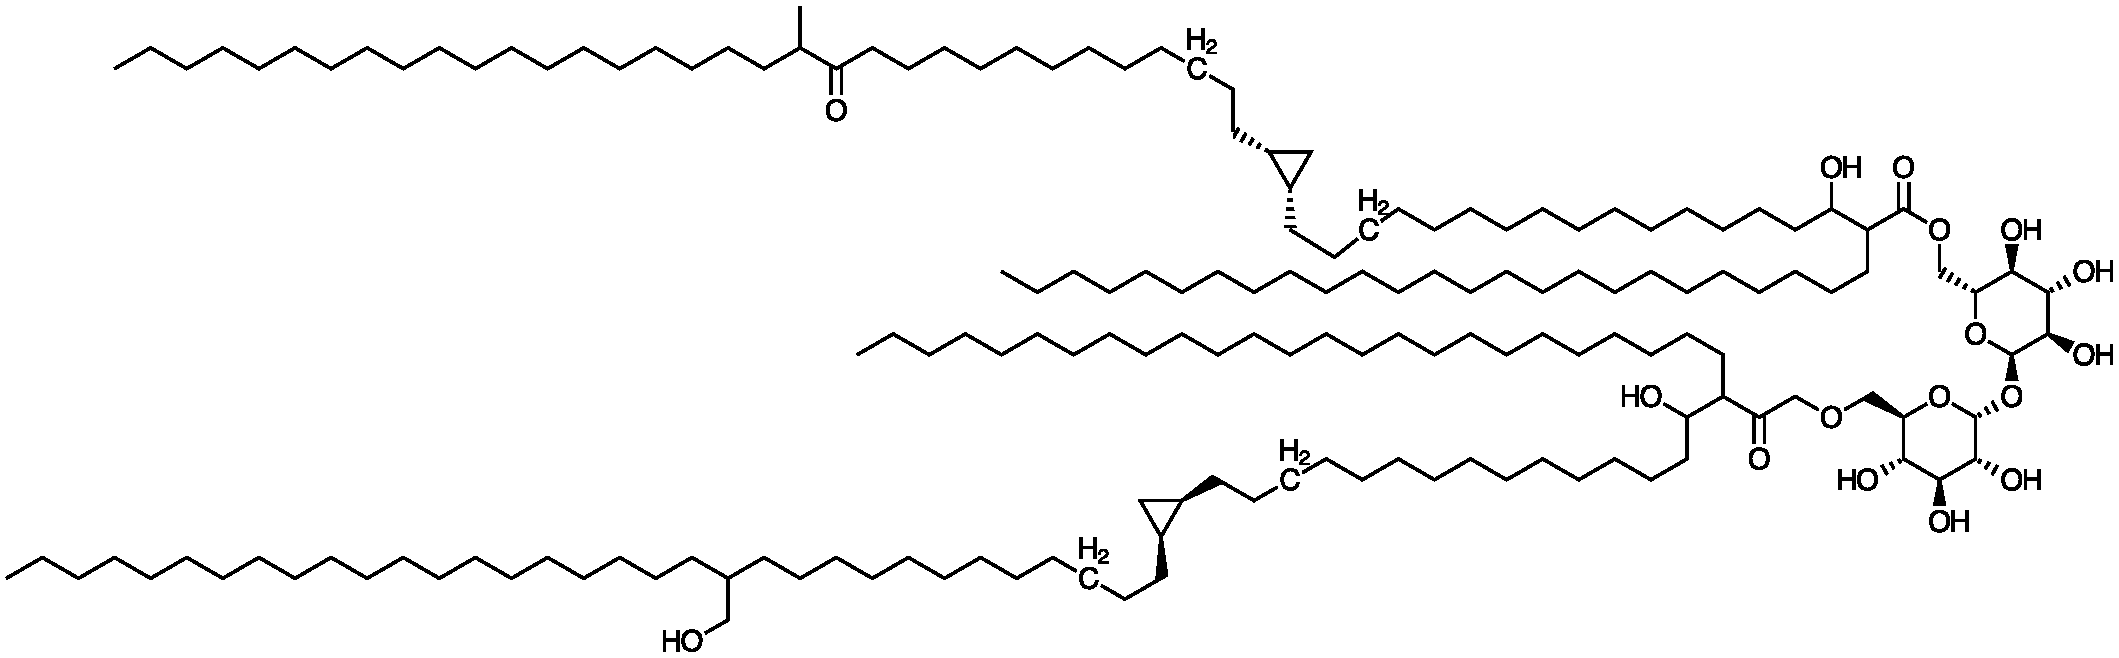
\includegraphics[width=\textwidth]{images/tdm.pdf}
\caption[Chemical structure of TDM]{TDM is the primary component of the mycobacterial cell wall and can be seen here. At defined locations along the length of the mycolate chains, modifications can be added by a set of defined enzymes. The most notable of these modifications are the unusual and biologically rare cyclopropane modifications, which provide TDM a number of immunomodulatory characteristics.}
% Provide a label so we can cross-reference it from the tex
\label{figure:tdm}
\end{figure}

TDM, in many ways, defines the lifestyle of mycobacteria. As mentioned previously, this remarkably hydrophobic (indeed, wax\hyp{}like) structure provides bacteria a potent tool for surviving not only harsh and fickle environmental conditions but also the conditions likely to be encountered in a host. This structure has been thoroughly dissected over the past decades of research, and a range of modifications are known that influence both the biochemical properties of the cell wall and the ways in which host organisms respond to this structure. Along the length of the mycolic acid tails, there are four main classes of modifications that may be present in two major locations. These modifications include methoxy, methyl, keto, and cyclopropyl groups, which can be located at either proximal or distal locations \citep{Sugawara2002, Minnikin2002, Takayama2005, Rao2005, Rao2006, Bhatt2008, Barkan2009, Walton2018}. Some of these modifications are represented along the structure shown in \autoref{figure:tdm}. Of these, the most research interest has centered on the very unusual cyclopropane modifications, which add a great deal of energetic ring strain to the molecule and are, generally, unusual biological modifications due to their inherent instability and energy investment required to create \citep{Wessjohann2003, Bach2004}.

Cyclopropane modification of the proximal modification site (at approximately C\textsubscript{16}) has been identified in both \textit{cis} and \textit{trans} isomers, each with distinct immunological properties and with both present within individual mycobacteria \citep{Glickman2000, Glickman2001a, Rao2005, Rao2006}. The \textit{cis} modification was described first and is added to TDM by the protein product of the bacterial gene \textit{pcaA}. \textit{M. tuberculosis} deficient in \textit{pcaA} is hypoinflammatory in a mouse model of infection, suggesting that \textit{cis}\hyp{}cyclopropane modified TDM is pro\hyp{}inflammatory \citep{Rao2005}. Loss of this gene results in an overall reduction in bacterial survival. This somewhat contradictory result indicates that aspects of the host inflammatory response are important for bacterial survival and replication, findings that have since been replicated in a variety of other contexts in respect to tuberculosis disease \citep{Koul2004, Flynn2005, Huynh2011, Sasindran2011, Tobin2012}. Alternately, \textit{trans}\hyp{}cyclopropane modification of TDM is catalyzed by CmaA2\footnote{Some redundancy is also seen with $\upDelta$\textit{mmaA2}, but these must have important different roles; MmaA2 also modifies the distal site of the mycolate chains \citep{Glickman2003, Barkan2010}.} and this orientation was found to be hypoinflammatory \citep{Rao2006}. Similar to $\upDelta$\textit{pcaA} \textit{M. tuberculosis}, loss of \textit{cmaA2} resulted in a bacterial growth defect and prompt clearance of the bacteria, but by an alternative mechanism. Instead of a muted inflammatory response, $\upDelta$\textit{cmaA2} \textit{M. tuberculosis} induced hyperinflammation. Loss of both ($\upDelta$\textit{pcaA}$\upDelta$\textit{cmaA2}) results in hyperinflammation as well, suggesting that \textit{trans}\hyp{}cyclopropanation is a mechanism to dampen detection and this modification predominates in the absence of \textit{pcaA} \citep{Barkan2012}. This body of work, largely from the Glickman lab, established a variety of important immunological roles for enantiomerically distinct versions of the same biomolecule that differ at only a single chemical site. This specificity is evocative of the high degree to which mycobacterial species have adapted to their hosts by developing novel modifications and mechanisms to perturb the immune response in their favor. By contrast, little has been described for roles of these modifications outside of modulating host immunity, suggesting that these may be innovations specific to the host\hyp{}pathogen interaction, especially as these enzymes are only present in pathogenic species and are absent from \textit{M. smegmatis}.

Models of TDM\hyp{}host cell interactions are often lacking by virtue of the underlying chemistry of TDM. The profound hydrophobicity of TDM limits the avenues by which it can be experimentally presented to cells\footnote{For instance, direct addition of TDM to tissue culture media would result in a film at the surface, or at best, seemingly inert micelles.}. On the surface of mycobacteria, TDM is (a) mixed with a range of other co\hyp{}stimulatory molecules that may be important for the function of TDM \citep{Rhoades2003, Torrelles2010, Mazurek2012}, (b) presented along the curved surface of a roughly\hyp{}cylindrical bacillus \citep{McCarter1935, Krokowski2018}, (c) constantly subject to remodeling as the chemically reactive components are oxidized \citep{Chan1989, Hett2010, Meniche2014, Shaku2020}, and (d) exists in different physical conformations based on the degree of bacterial cording and abundance of dead mycobacteria\footnote{I hypothesize that TDM exerts distinct functions in early and late infection -- early on, manipulation of the phagocytic macrophage is likely to be essential while in late infection it may be more important to modulate granuloma macrophages in the context of larger bacterial burden. Thus, it is sensible to think that the presentation on single bacilli and that on large clumps of bacilli may activate different receptors to different degrees. This is supported by analogy to \citet{Goodridge2011} but strict demonstration is likely to be challenging with existing tools and models.}. \textit{In vitro}, these are difficult aspects to model and two major methods have emerged to agonize cultured cells with TDM: on the surface of polystyrene microbeads \citep{Bloch1950, Retzinger1982, Behling1993, Indrigo2003, Geisel2005, Bowdish2009} and through evaporative monolayers on the surface of tissue culture plastic \citep{Schabbing1994, Hunter2006a, Harland2008, Ishikawa2009, Miyake2013, Zhao2014}. On beads of a small ($<$5 $\upmu$m) diameter or in aqueous micelles, it adopts a bilayer configuration somewhat similar to that seen on live individual bacilli; on larger beads or on a plane, it acts as a monolayer. The monolayer configuration is more inflammatory but was also thought unlikely to exist \textit{in vivo}, although this is subject to debate and cording may be a mechanism of mimicking this presentation based on the stage of the infection. Additionally, both interpretations rely on pure TDM in the absence of the complete milieu present on live mycobacteria; the inverse (removal of TDM from otherwise complete lipids) may be yet more informative as to the role of this unique compound.

While no comprehensive comparison between these exposure routes has been done, vague historical descriptions assign them two different behaviors. Dense surface monolayers of TDM are cytotoxic to cells and trigger a highly inflammatory response \citep{Retzinger1982, Schabbing1994, Hunter2006a, Welsh2013}; on the other hand, TDM on the surface of beads (although with some variation based on the diameter) tends to drive a more regulated response that still differs in some regards from that induced by whole, metabolically inactive mycobacteria \citep{Bowdish2009, Welsh2013}. While whole mycobacteria undoubtedly have other molecular patterns that augment the overall immune response, it is likely that the full breadth of the immune response to TDM has yet to be fully uncovered on account of deficient models to do so\footnote{Some model of total lipid reconstitution on freely associating bacillus\hyp{}sized beads within an extracellular matrix may get us closer to this -- isolating lipid activity in a native context but in the absence of confounding bacterial physiology \citep{Retzinger1982, Rhoades2003, Sakamoto2010}.}. The physiological relevance of these monolayer\hyp{}like configurations of TDM is up to some debate, but there is some evidence that planes of TDM from dead mycobacteria can form in vivo \citep{Schabbing1994, Hunter2006b, Glickman2008}. Additionally, the clumps of bacteria that form within the necrotic core may grow in larger macrostructures resembling these artificial planes. Despite the relative opacity of these historical observations, what is clear is that TDM must be presented to cells in particular arrangements to have particular effects, which is seen in head\hyp{}to\hyp{}head comparisons between heat\hyp{}killed \textit{M. tuberculosis} and gamma\hyp{}irradiated \textit{M. tuberculosis} \citep{Datta2006, Cha2015, Gleeson2016, Yang2018, Krokowski2018, Mosavari2021}. While gamma\hyp{}irradiated \textit{M. tuberculosis} maintain their shape and structure, heat\hyp{}killed \textit{M. tuberculosis} are broken down, dampening their ability to stimulate the immune system \citep{Carpenter1959, SecanellaFandos2014}. 

\subsubsection{Moonlighting}\label{moon}

Pathogenic microorganisms are often constrained by genomic size -- too small and too few essential functions can be encoded; too large and the risk of duplication errors and energetic cost of maintenance becomes prohibitory \citep{Ranea2005, Huberts2010, Bobay2017}. There is therefore a great deal of evolutionary pressure to economize and multitask -- why have two proteins to do two functions if one can do both? That is the precise logic underlying many bacterial toxins, secreted effectors, and structural features \citep{Gupta2019}. One of the most famous of these multifunctional proteins, often dubbed moonlighting proteins\footnote{Conceptually, of course, moonlighting is purely orientational. While the given example is one instance where a historically well\hyp{}defined enzyme has additional functions based on localization, other multifunctional enzymes that can target both bacterial and host substrates or that have distinct functions when cytosolic or periplasmic or secreted are unlikely to be given this title unless they bear high homology to universally conserved proteins.}, is the alpha\hyp{}enolase from \textit{Streptococcus pneumoniae} \citep{Bergmann2001}. Enolase is an enzyme critical to glycolysis and converts 2\hyp{}phosphoglycerate to phosphoenolpyruvate, which is an essential intermediate in the breakdown of glucose into pyruvate to generate ATP and NADH. However, \textit{S. pneumoniae} also secretes this normally cytosolic enzyme onto the surface of the outer membrane, which allows it to interact with host plasminogen and catalyze its conversion into active plasmin \citep{Bergmann2013}. Plasmin degrades host fibrin clots, leading to enhanced tissue invasion and pathogenicity through avoidance of pathogen containment by host fibrin and increased dissemination \citep{Whiting2002, Weiser2018}. By evolutionary addition of new properties, fusion of two unrelated proteins into a single protein, alterations of protein localization, or novel layers of regulation, bacteria can, in a very efficient way, exert multiple essential functions from single biological products.

Within mycobacteria, there are many notorious examples of ``moonlighting'' proteins, including the enolase of \textit{M. tuberculosis}, which also binds plasminogen\footnote{As will become relevant later in this document (\autoref{plg}), plasmin also has important regulatory function during angiogenesis. How mycobacterial engagement of plasmin(ogen) alters the overall angiogenic response is an interesting question that warrants future study.} \citep{Rahi2017}. Indeed, enolase appears to be a highly conserved moonlighting protein, with plasminogen binding having been demonstrated for numerous other species as well \citep{Seweryn2007, Vanegas2007, Agarwal2008, Candela2009, Floden2011, Figueiredo2015}. \textit{M. tuberculosis} has other metabolic enzymes that are used to subvert the host immune response. For instance, mycobacterial MenJ is a vitamin K oxidoreductase that confers intracellular survival within macrophages independent of its catalytic activity \citep{Kumar2020b}. Similarly, ArgD is an acetylornithine aminotransferase that also acts as a potent TLR4 agonist \citep{Nehvi2022}. This repurposing of metabolic enzymes is one of many notable ways of subverting host immunity while optimizing genetic coding space \citep{Banerjee2004, Banerjee2007, Henderson2010}. Given that \textit{M. tuberculosis} has lost approximately 30\% of its genomic content relative to environmental mycobacteria, streamlining has played an important role in adaptation to an exclusively pathogenic lifestyle \citep{Stinear2008}. 

Similar to protein examples, which tend to be more obvious, the structural features of the bacteria can also serve important moonlighting functions in the sense that single compounds can play key roles in seemingly unrelated phenomena. TDM is an excellent example of this -- it is a conserved feature of non\hyp{}pathogenic mycobacterial species, suggesting that this feature likely emerged to address environmental needs that preceded the need to engage with host immunity \citep{Kremer2002, Pacheco2013}. However, the adaptation to a pathogenic lifestyle has resulted in TDM being repurposed with additional modifications to suit these new demands. Indeed, TDM serves such a wide array of important functions in the physiology of (especially pathogenic) mycobacteria that to assign it a ``major'' function would be rather fallacious. As a major structural component of the cell wall, defense from the environment, broadly speaking, is clearly the overarching theme of this sophisticated glycolipid. 

Strictly in the context of host immunity, TDM had been generally ascribed a few major roles: (a) blockade of lysosomal\hyp{}phagosomal fusion \citep{Indrigo2003, Axelrod2008, Patin2017b}, (b) alteration in expression of major immunoregulatory cytokines \citep{Perez2000, Indrigo2002, Bowdish2009, Sakamoto2013}, (c) induction of humoral immunity \citep{Fujiwara1999, Ryll2001, Fujita2005}, (d) stimulation of hypercoagulation \citep{Retzinger1982, Retzinger1987, Donnachie2016}, (e) interaction with the stromal milieu \citep{Sakamoto2010}, (f) mediation of granuloma formation \citep{Bekierkunst1968, Hunter2006b, Lee2012}, and more. Delipidation of mycobacteria results in a profound alteration of the overall inflammatory response \textit{in vitro} and results in efficient bacterial killing by macrophages but perturbed expression of IL\hyp{}1$\upbeta$, TNF\hyp{}$\upalpha$\footnote{TNF\hyp{}$\upalpha$ was once commonly called ``cachectin'' for its ability to induce cachexia \citep{Tracey1988}. TNF\hyp{}$\upalpha$ is probably the defining cytokine of tuberculosis infection and is critical for bacterial control \citep{Orme1998}, although others may, with equal validity, argue that this honor goes to IFN\hyp{}$\upgamma$.}, IL\hyp{}6, and IL\hyp{}12. It is now thought that many of these functions are mediated by recognition of TDM by surface host receptors\footnote{Whether or not these receptors detect mycobacteria within the phagosome is unknown -- this may be able to explain some, but not all, of the influence of TDM on infected macrophages.}, a topic that will be returned to shortly. However, the expression of these critical cytokines (among many others) regulated by TDM results in profound changes in the overall tone and tempo of the inflammatory response that, in aggregate, contribute to granuloma formation, a process we now know to be dependent on both pro\hyp{} and anti\hyp{}inflammatory signaling molecules, including IL\hyp{}4, IL\hyp{}13, IFN\hyp{}$\upgamma$, TNF\hyp{}$\upalpha$, and nitric oxide \citep{Flynn1993, Cooper1993, Bergeron1997, MacMicking1997b, Kaneko1999, Akdis2011, Cavalcanti2012, Cronan2021}. These processes are intimately linked with the phenotype that will be further explored throughout this work: the TDM\hyp{}dependent induction of VEGFA within granuloma macrophages and resultant neighboring angiogenesis.

\section{Macrophages in Development and Disease}\label{macrophages}

Macrophages are developmentally essential for the survival of vertebrate organisms. These phagocytic cells of the hematopoietic lineage perform vital roles in organ development, immune maturation, vascular remodeling, scavenging for cellular debris, and defense against pathogens \citep{Wynn2013, Wattrus2022}. They are both continually replenished by hematopoiesis in the bone marrow and migration into destination tissues as well as self\hyp{}renewing within essentially every tissue in specialized form -- microglia in the brain, alveolar macrophages in the lung, Kupffer cells in the liver, osteoclasts in the bone, Langerhans cells in the skin, histiocytes in connective tissue, and varying generically\hyp{}named macrophages in the heart, blood vessels, adipose tissue, lymphatic tissue, gonads, and the intestinal tract \citep{Davies2013a, Bain2018, Na2019}. Under normal conditions, these macrophages circulate through the blood as precursors known as monocytes which, themselves, have important roles in immunity \citep{Sampath2018, Mass2018}. Upon activation by an outside stimulus, these monocytes will extravasate and undergo tissue\hyp{}educated differentiation into macrophages. Macrophages are the central orchestrators of immunity to tuberculosis, acting as the first responders and comprising the host\hyp{}pathogen interface, being the primary cellular constituent of the granuloma \citep{Pagan2018}. These macrophages must be capable of both initiating and resolving inflammation, finely tuning their responses dynamically over the course of an insult in order to simultaneously clear invading pathogens, limit the pathology of inflammation, and ultimately repair damaged tissues \citep{Unanue1987, Murray2011, Watanabe2019}.

\subsection{The M1\hyp{}M2 (False) Dichotomy}\label{lies}

For the past two decades, macrophage research has been dominated by the concept of the M1\hyp{}M2 binary of polarization states \citep{Italiani2014, Mills2015}. This concept, introduced by \citet{Mills2000} is a useful paradigm to understand the activity of macrophages \textit{in vitro} and mirrors certain aspects of \textit{in vivo} biology, but proves inadequate to capture the diversity and ironies of macrophage behaviors. M1 macrophages are described as ``classically'' activated and are produced in response to TLR agonists (see \autoref{prrs} for more details) and IFN\hyp{}$\upgamma$ while M2(a) macrophages differentiate in response to IL\hyp{}4/IL\hyp{}13 \citep{Wynn2013, Mills2014}. This neatly classifies these macrophages into inflammatory and anti\hyp{}inflammatory in a deliberate parallel to the T\textsubscript{H}1/T\textsubscript{H}2 T cell paradigm. Further research has identified a number of subtypes of M2 macrophages, including M2b (immune complexes, IL\hyp{}1, TLR agonists), M2c (IL\hyp{}10, TGF\hyp{}$\upbeta$, glucocorticoids), and M2d (IL\hyp{}6, TLR agonists, adenosine) \citep{Huang2018, Viola2019}. What this research has revealed is that macrophages are fascinatingly diverse cells, able to respond intelligently to different stimuli and dynamically alter their responses through integration of new information. In the era of single cell RNA sequencing and an ever\hyp{}greater number of single cell \hyp{}omics approaches, it has become apparent that \textit{in vivo}, this binary does not exist. These subtypes are defined based on their treatment \textit{in vitro} with a limited and defined subset of stimuli \citep{Wynn2013, Gosselin2014}; in a tissue context, cells are continually bombarded with often conflicting signals that they must synthesize to create a coherent set of actions \citep{Murray2014} and macrophages are imprinted by their phagocytic history, generating further layers of heterogeneity \citep{Gonzalez2017}. What has been proposed instead, by \citet{Nahrendorf2016} in a beautiful opinion piece, is a network of macrophage activation possibilities that realistically acknowledges the limitations of the current model. Macrophages are capable of expressing both M1 and M2 signatures simultaneously in ways that defy typical classification, but if only a limited subset of markers are assessed, then a macrophage population may be erroneously deemed ``M1'' or ``M2''. This limits the degree to which the dominant M1\hyp{}M2 model is able to reflect any real biology \textit{in vivo}. 

While this M1\hyp{}M2 nomenclature will inevitably come up throughout the course of this thesis, it is suggested that any in\hyp{}text use be taken as a pure reflection of the historical context of the publication being cited and lack of additional information to call them otherwise \footnote{The distinctions between different T cell differentiation states appear to be more in line with proper differentiation and not simply activation. Type I responses are those that induce inflammation while type II responses are responsible for tolerance and resolution. There are additional T cell activation states (many of them) that reveal some of the discrete loci along the gradient which immune responses can exist. This is beyond the scope of the present work, but I am not denying the existence of immune polarization and type responses, merely the binary classification of the highly plastic macrophages based on highly controlled \textit{in vitro} exposures to defined cytokines.}. I will not use these terms to describe any of the macrophages in the experiments presented in Chapter 3 and this choice is deliberate in pursuit of understanding the biology of the macrophage, not simply what it might be called.

\subsection{Developmental Origins}\label{macdev}

Two cell types are a ubiquitous presence in every tissue in the body: endothelial cells and macrophages. These two tissues serve as the support system for all other bodily functions. The endothelium does so by providing oxygen and nutrients to these tissues, as well as providing a signaling infrastructure to alter tissue development and homeostasis\footnote{The relative contributions of these two cell types to development have largely been revealed by the differential lethality of mutations affecting these individual systems, which both arise from a common hemangioblast precursor that was implied by the existence of the \textit{cloche} mutation \citep{Stainier1995, Vogeli2006}. Mutation in \textit{myb} result in a total loss of blood cells, but this is viable into adult stages of development in the zebrafish \citep{Lipsick2010, SozaRied2010}. By contrast, loss of the two homologs of \textit{VEGFA} in the zebrafish (\textit{vegfaa} and \textit{vegfab}) or the \textit{kdrl} receptor results in embryonic lethality \citep{Carmeliet1996}. These will be discussed slightly more in \autoref{zfhist}.}. Macrophages, on the other hand, serve to actively maintain tissue structure and health through the production of a range of cytokines, chemokines, and signaling molecules and patrol tissues to clear cell debris \citep{Wynn2013}. During infection or other tissue damage, these tissue\hyp{}resident macrophages are able to quickly respond to eradicate most invaders and return the tissue to homeostasis. Macrophages are also intimately involved in the development of most or all tissues and emerge early in embryonic development to serve in this role.

Macrophages first emerge from the yolk sac via primitive hematopoiesis at approximately six weeks post fertilization in humans \citep{Geissmann2010, Yona2013, Feyaerts2022}. Each of these in its own tissue is essential for remodeling and homeostasis both in early embryonic development and in developmental processes throughout life as they self\hyp{}renew in addition to contributions from circulating monocytes \citep{Jappinen2019}. Microglia, the first of these to emerge, are important for response to neurological damage and scavenge for cell debris; developmentally, they are important for synaptic pruning and maturation for the solidification of knowledge and behavior \citep{Wynn2013, Lavin2015}. In the absence of microglia, synapses grow unrestricted and form aberrant connections in a way that mirrors the the immature brain and greater numbers of neurons develop and survive but lack mature synapses indicative of cohesive pruning \citep{Hammond2018}. And, in a theme that will be present throughout different contexts, these macrophages are important for the elaboration of the brain vasculature. Microglia secrete VEGFA to guide the production of blood vessels throughout the brain; given the sizable demands of the brain for oxygen and glucose, this is a patently important role for these cells from the earliest stages of life \citep{Dudiki2020}. 

Subsequently, other types of specialized macrophages emerge and populate other organs, including Langerhans cells, Kupffer cells, and alveolar macrophages \citep{Davies2013a, Wynn2013, Lavin2015, Gordon2017}. These macrophages must all deal with the environment at large either through direct contact in the airway or the skin or indirectly via toxin processing in the liver. Langerhans cells are important for immediate host defense against invading pathogens at the skin and are additionally required at homeostasis for important self\hyp{}renewal processes, including hair growth and skin shedding \citep{Merad2008, Theret2019}. Kupffer cells are responsible for modulating liver filtering functions, including by modulation of liver uptake of cholesterol; they are also able to combat pathogens and facilitate the removal of dying cells and are important for liver regeneration \citep{Theret2019, Demetz2020}. 

Alveolar macrophages -- the primary tissue\hyp{}specific macrophage subtype of interest in tuberculosis -- are extremely plastic cells that are essential for the maintenance of lung health both from natural cellular turnover in the lung and resorption of pulmonary mucus and due to the abundance of potential respiratory pathogens faced in the daily life of any lunged animal \citep{Hussell2014}. Alveolar macrophages are self\hyp{}renewing and, after establishment from the yolk sac during development, are capable of perpetuating themselves throughout life with only modest contributions from circulating monocytes \citep{Hashimoto2013, Yona2013, Varol2015}. Inflammation in the lungs is clearly harmful for normal bodily functions and hyper\hyp{}inflammation is a death knell \citep{Kemp2002}. Thus, alveolar macrophages must finely tune their responses to pathogens and lung damage to facilitate pathogen clearance and tissue repair. In general, alveolar macrophages have a muted inflammatory immune response \textit{in vitro}\footnote{Although it is relatively easy to harvest alveolar macrophages by bronchoalveolar lavage, providing them a stable environment \textit{ex vivo} seems to be rather challenging. While this is the closest that can be gotten to \textit{in vivo}, this too comes with some caveats.}, evocative of their delicate role in maintaining lung function \citep{Joshi2018, Svedberg2019}. Like most other tissue\hyp{}resident macrophages, these cells evade clear classification on the M1\hyp{}M2 polarization axis and can span the full range of these phenotypes depending on the circumstance and in response to cytokines generated by other cells \citep{Hussell2014, Svedberg2019}. 

In their particular tissues, all of these macrophage subsets are responsible for both inducing inflammation and resolving it. These cells must plasticly respond to ever\hyp{}changing conditions to exact the proper type of response at the appropriate time \citep{Pollard2009}. They must also change over the course of the life of the organism, transitioning from early roles in aiding the development of tissues to maintaining homeostasis and, eventually, managing the aging process \citep{Linehan2015, Duong2021, Guimaraes2021, DeMaeyer2021}. An interesting additional role for macrophages that is just beginning to be studied is their capacity to physically transmit signals between tissues. A recent study found that pigment cells in the zebrafish were remodeled based on interactions with macrophages and, in their absence, melanocyte patterning is disrupted. This argues that macrophages, via their intrinsic motility, may be able to augment long\hyp{}range communications to facilitate tissue remodeling and repair \citep{Eom2017}. Macrophages also exist at the very foundation of immune system development, being the master regulators of hematopoietic stem cell survival, thus determining the clonal populations that contribute to all hematopoietic lineages throughout life \citep{Wattrus2022}.

\subsection{Alveolar Macrophages in Tuberculosis}\label{alvmac}

Alveolar macrophages are the first responders to tuberculosis infection, being already present at the site \citep{Flynn2001}. Their biology is fundamentally a reflection of the niche in which they reside -- they utilize oxidative phosphorylation as a metabolic modus to take advantage of the abundant oxygen present and respond modestly and slowly to insult as a means to minimize pathology \citep{Joshi2018}. These macrophages are thus of great interest for the roles they play in the overall pathogenesis of \textit{M. tuberculosis}. Alveolar macrophages have been shown to be more susceptible to infection by mycobacteria, in general, than are the interstitial macrophages to soon arrive at the site, in part due to their mixed activation state and delayed responses \citep{Kahnert2006, Madden2022}, although circulating monocytes appear to be more susceptible still \citep{Cambier2014b, Cambier2017}. Early studies found that \textit{M. tuberculosis} induces apoptosis of alveolar macrophages to facilitate their escape into the interstitial space \citep{Keane1997}; further study actually uncovered that, although virulent \textit{M. tuberculosis} was able to induce apoptosis, it actually did so \textit{less} than avirulent strains, suggesting that some virulence factor limited apoptosis to provide the bacteria a temporary replicative niche \citep{Keane2000, Cohen2018}. Subsequent findings on apoptosis as a host\hyp{}protective response align well with these data and necrosis is \textit{M. tuberculosis}'s preferred means of cellular exit from macrophages \citep{Behar2011}, much of which is interconnected with the process and consequences of efferocytosis by other innate immune cell types \citep{Martin2012}. Some of the foundational studies on \textit{M. tuberculosis} macrophage subversion were in the specific context of alveolar macrophages; \citet{Mwandumba2004} found that the bacteria are able to reside in pH\hyp{}neutral phagosomes within alveolar macrophages, allowing them to survive and replicate. Consistent with these findings, it was uncovered that depleting alveolar macrophages actually results in improved bacterial control, implicating alveolar macrophages as a weak link in the overall response to tuberculosis -- shielding the bacteria until their population had expanded beyond the reasonable limits of control able to be exerted by recruited macrophages and neutrophils \citep{Leemans2001}. 

These infected macrophages are also able to shuttle the bacteria out of the lung and into the interstitium, an event that long precedes bacterial infection of other cell types and the establishment of a productive infection \citep{Cohen2018}. However, alveolar macrophages from patient contacts have increased capacity to restrict bacterial growth, perhaps in an instance of ``trained immunity''\footnote{The concept of trained immunity or innate immunological priming is an interesting concept that has been put into use (largely by accident) for decades. While it is beyond the scope of the present work to give it is proper discussion, further reading can be found at \citep{Arts2018, Moorlag2020, Khan2020, Netea2020, Katzmarski2021, Trauer2021, Kaufmann2022, Katzmarski2022}. The mechanism of BCG in the treatment of bladder cancer is largely through trained immunity \citep{RedelmanSidi2014} and BCG is being evaluated as a trained immunity vaccine against COVID\hyp{}19 and potentially future pandemics for which no specific vaccine yet exists \citep{RedelmanSidi2020}.} exerting protective effects after sub\hyp{}clinical exposure \citep{Carranza2006, Divangahi2021}. 

If alveolar macrophages are such poor responders to tuberculosis, are other cell types better able to control the infection? This has been a critical question in the development of new therapeutic options. While a thorough discussion of what is known about neutrophils is beyond the scope of this work, the general conclusion on the role of neutrophils in the pathogenesis of tuberculosis infection has been equivocal, with different groups using different models coming to disparate and difficult\hyp{}to\hyp{}reconcile conclusions \citep{Fortune2007, Yang2012, Srivastava2014}. On the other hand, the critical importance of hematopoietic\hyp{}derived macrophages is clear: these cells are absolutely required for the effective control of tuberculosis infection and, in their absence, bacteria grow uncontrolled in the host \citep{Clay2007, Pagan2015, Matty2019}. 

\subsection[Recruited Macrophages in Tuberculosis]{Recruited Macrophages in Tuberculosis\footnote{While books could be written on the body of \textit{in vitro} macrophage responses during infection, I have deliberately attempted, with varying success, to narrow the focus onto known \textit{in vivo} biology to aid in differentiating macrophages by their ontogeny.}}\label{recmac}

At homeostasis, non\hyp{}tissue resident macrophages circulate through the blood stream as monocytes. While these comprise a minority of the total macrophages in the body, they are key respondents to sites of insult to mediate pathogen control and wound healing. In the classical model, these then differentiate into more M1\hyp{}like macrophages, expressing IFN\hyp{}$\upgamma$, TNF\hyp{}$\upalpha$, and IL\hyp{}1$\upbeta$ \citep{ArangoDuque2014}. Despite their critical importance, relatively little is actually known about the biology of macrophages derived from circulating monocytes in the initial events of the immune response to tuberculosis. For the first fifteen days of infection (in mice), the entire course of infection is dictated by alveolar macrophages, which are the near\hyp{}exclusive hosts of mycobacteria until that time point, at which time monocyte\hyp{}derived macrophages and neutrophils become the major host cells \citep{Cohen2018}. Recruited monocytes sense a number of chemoattractants to direct them to the site of infection and then differentiate into macrophages, including type I interferon and CCL2 \citep{Peters2001, Peters2004, Antonelli2010, Desvignes2012}. \citet{Antonelli2010} concluded that the recruitment of these macrophages exacerbated infection as these were pathogen\hyp{}permissive cells; however, this paints a picture of \textit{all} macrophages as being detrimental for disease when synthesized with the findings from \citet{Leemans2001}, who found that alveolar macrophage depletion ameliorated disease. What to make of this then? It appears that macrophage\hyp{}derived type I interferons (IFN\hyp{}$\upalpha$/$\upbeta$) are, indeed, detrimental during tuberculosis and engage in discrete functions from the classically protective IFN\hyp{}$\upgamma$. Additionally, CCR2 is an important protective chemokine through its ability to recruit interstitial macrophages to the lung \citep{Peters2001}, although the net effect of this appears to result overall in worse disease outcomes \citep{Cambier2014b}. Many of the ultimate effects are ascribed to a failure to recruit T cells after infection, but clearly there are potentially essential roles for these recruited macrophages in directly protecting against tuberculosis. 

Much of what we know about the interactions between macrophages and pathogenic mycobacteria come from \textit{in vivo} observations in the zebrafish model\footnote{For now, this is the extent of required detail. More will be provided in \autoref{zebrafish}, but suffice to say that, given all that is known about the differences in \textit{in vitro} and \textit{in vivo} macrophage biology, this serves as a surrogate, optically accessible host for studying the earliest events of infection in a native tissue context.}\footnote{There are many studies of the \textit{in vitro} interactions between macrophages and mycobacteria. These are extremely valuable studies that model important aspects of these interactions that have later been demonstrated to be critical \textit{in vivo}. I will focus on those findings that are directly relevant to the \textit{in vivo} context for these purposes.} Genetic depletion of all of the macrophages in the developing zebrafish larva results in unrestricted growth of bacteria, suggesting that patrolling macrophages are important mediators of host protection during the earliest events of infection \citep{Clay2007}. Similar to the findings from \citeauthor{Cohen2018}, it was found that these macrophages are important for the dissemination of the bacteria into other tissues; it is possible that macrophages are broadly able to fulfill this role depending on the particular disease context and alveolar macrophages happen to be the population of interest in pulmonary tuberculosis. These findings contrasted with those found in previous models, where wholesale depletion of all macrophages in the mouse lung was able to decrease bacterial burden \citep{Leemans2005}. Further, it is clear from human population studies that macrophage deficiencies increase susceptibility to tuberculosis \citep{Hambleton2011}, although functional differences in macrophage ``deficiency'' and macrophage eradication are obviously possible, as are unintended consequences of genetic mutants that are unrelated to their effects on macrophage number. Nevertheless, the aggregate of these data demonstrates that patrolling macrophages recruited to the site of infection can exert protective activity against tuberculosis while resident alveolar macrophages are unable to do so on account of their tissue\hyp{}specific niche and more limited microbicidal activity.

These data evoke the roles of macrophages in ``undisturbed'' tuberculosis infection, but a comprehensive analysis must integrate the existing therapies used to treat tuberculosis, especially in the context of drug\hyp{}resistant strains. Much ink has been spilled on the role of the granuloma as a physical barrier to therapeutic access during infection \citep{Driver2012, Ekins2014, Cicchese2020, Cronan2022}, but \citet{Adams2011} identified a role for macrophage drug efflux in inducing drug tolerance in mycobacteria. By allowing the bacteria to grow undisturbed while being exposed to bactericidal concentrations of antitubercular drugs, the macrophages can act as a protective niche against treatment. While these roles clearly did not evolve on account of the modern treatment regimen, they reveal an interesting dimension of the cell biology of the bacteria, wherein macrophages actively efflux drugs that ultimately protects the pathogen; notably, treatment with efflux pump inhibitors lowers intra\hyp{}macrophage bacterial burden by increasing the effective drug concentration. Experimentation to identify whether this process is similarly protective against metallotoxicity or other endogenous factors would provide further context to the evolutionary origins of this phenomenon.

\subsection{Host Resistance and Susceptibility to Infection Mediated by Macrophages}\label{macsig}

Macrophages play extremely complex and often contradictory roles in the control of infection based on their responses at particular times along a very fine gradient, where seemingly subtle shifts can result in radically different functional outcomes. While there is a great deal known about outright susceptibility to infection, including the Mendelian susceptibility to mycobacterial disease, which is caused by errors in the response to IFN\hyp{}$\upgamma$ \citep{Bustamante2014}, many or most of these levels of resistance are likely to be mediated by macrophage behaviors, which are certain to be the major player for any response that does not stimulate an adaptive response detectable by skin test. Particular genetic disorders are known to lead to increased susceptibility to mycobacterial infections, including normally opportunistic mycobacteria. For instance, lysosomal storage disorders alter macrophage behavior and migration to increase patient susceptibility to tuberculosis \citep{Berg2016}. More general approaches have also been taken to identify macrophage genes that mediate susceptibility to tuberculosis \citep{Thuong2008}, but this remains a field worth additional exploration. 

There is an enormous body of literature on the contributions of macrophages in the general execution of control in tuberculosis infection. Although literature descriptions tend to focus on the many ways that the bacterium can subvert the capacity of the macrophage to kill it, the previously detailed evidence on the consequences of macrophage depletion suggest that macrophages are capable of some level of effective control \citep{Pagan2015}. Macrophages natively express a spectrum of pattern recognition receptors (PRRs), genetically encoded receptors that bind discrete ligands from bacteria, viruses, fungi, parasites, and damaged\hyp{}self which allows cells of the innate immune system to discriminate between self and non\hyp{}self. These receptors are not only capable of activating the macrophage to execute more effective antimicrobial functions, they also serve as a critical step in macrophage antigen presentation for the purpose of stimulating a potentially protective adaptive response. 

The earliest studies on this topic identified a set of cytokines that were clearly important for the control of tuberculosis: TNF\hyp{}$\upalpha$, IFN\hyp{}$\upgamma$, and IL\hyp{}12 among them \citep{Flynn1993, Cooper1993, Flynn1995, Cooper1997}. Further studies on human genetics found that variations in the NRAMP1 gene conferred resistance to tuberculosis infection \citep{Bellamy1998}, perhaps through increased metal ion transport into the phagosome \citep{Davies2001a}. Similarly, polymorphisms in the promoter for hepcidin, which regulates iron transport, alter susceptibility to disseminated tuberculosis \citep{Liang2017}. Indeed, one of the major functions of IFN\hyp{}$\upgamma$ and TNF\hyp{}$\upalpha$ is to further activate macrophages to execute bactericidal control \citep{Kaufmann2002}. TNF\hyp{}$\upalpha$ is also essential for the development and stability of granulomas in the mouse, presenting a multifaceted role for this critical cytokine \citep{Chakravarty2008}. Despite the classical model of mycobacterial blockade of phagosomal\hyp{}lysosomal fusion, some cells manage to complete this fusion and kill the contained mycobacteria \citep{Kaufmann2002}. 

Subsequent studies have revealed additional macrophage gene products that undermine the host immune response and serve important bacterially beneficial roles. Two of these -- CCL2 and MMP9 -- are important for recruiting additional macrophages and restructuring the interstitial microenvironment \citep{Volkman2010, Cambier2014b}. Due to the liabilities impose by these genes on the progression of disease, it seems plausible that targeting them may offer an alternative path for disease treatment. Additionally, unlike previous studies, these offer unequivocal host susceptibility responses; knockout of IFN\hyp{}$\upgamma$ or TNF\hyp{}$\upalpha$ result in increased bacterial burden and defective granuloma formation whereas abolition of MMP9 and CCL2 resulted in reductions in both granuloma formation \textit{and} bacterial burden.

Other signaling events can also play important roles in host defense against tuberculosis infection, especially other aspects of the cytokine environment that can exact control of mycobacteria. One of the most recently described of these is the capacity for GM\hyp{}CSF to activate macrophages to control bacterial replication, a process that is inhibited by HIV\hyp{}1 coinfection \citep{Bryson2019}. Interestingly, addition of GM\hyp{}CSF to the macrophages facilitates renewed control, suggesting that cytokine re\hyp{}regulation may be an avenue for new therapies as it is in many other chronic infections; by returning the milieu to a proper tone, it may be possible to encourage macrophages to kill the bacteria more effectively despite the measures taken by the bacteria or comorbidities to prevent this outcome. The nature of macrophages during HIV infection is an interesting question given that these cells can be directly infected by the virus and that tuberculosis is such a common and severe disease among AIDS patients. Alveolar macrophages display altered activation status and serve as a reservoir for HIV, which compromises the earliest events of the response to infection \citep{Evans1996, Herbein2002, Cassol2010, Cribbs2015, Clayton2017, Kruize2019}. These alterations make the macrophages resistant to killing by cytotoxic T lymphocytes as well as impaired for the induction of key anti\hyp{}inflammatory responses \citep{Porcheray2006, Herbein2010, Clayton2018, Neff2020}. Together, the increased susceptibility to tuberculosis infection during AIDS results in combinatorial innate and adaptive immune suppression that leads to rapid disease progression due to the effects of HIV in killing CD4\textsuperscript{+} T cells and modulating macrophages responses with mycobacterial killing of macrophages within the lung \citep{Mariani2001}.

Non\hyp{}proteinic signals can also intersect with these events, including nitric oxide, hydrogen sulfide, and superoxide, which are widely produced metabolites that have many functions in homeostasis and disease. Nitric oxide is a potent vasodilator\footnote{Nitric oxide release is the primary mechanism of action for nitroglycerin treatment during infarction.} and oxidant that is able to kill mycobacteria, but also prevents the infiltration of pathogen\hyp{}permissive neutrophils into the granuloma, reducing bacterial burden \citep{MacMicking1995, MacMicking1997a, MacMicking1997b, Szabo2007, Mishra2017b}. Hydrogen sulfide also acts in an immunosuppressive fashion and prevents macrophage\hyp{}mediated inflammation and reduces production of protective cytokines, but this suppressive phenotype results in increased bacterial burden \citep{Rahman2020}. Superoxide production promotes tolerance to infection to sustain host survival even at the same bacterial burden, a new and more complex role for these simple compounds on determining host outcomes \citep{Olive2018}.

Macrophage cell death pathways can play important roles in priming later steps of protection. Through the process of necrosis or necroptosis, macrophages release bacteria into the tissue to infect new macrophages, a process that the bacteria actively exploits through production of TNT\footnote{For many years, tuberculosis was thought to lack traditional toxins that define the pathogenicity of many other bacterial pathogens, such as \textit{Shigella} and \textit{Vibrio cholerae} \citep{Holmgren1981, Tesh1991, Gyles2007, Guichard2013}. However, recent findings have identified the existence of the tuberculosis necrotizing toxin, or TNT, a subunit of the outer membrane protein CpnT that can be cleaved off and exported into the host macrophage where it induces an immunologically blunted necrosis, allowing the bacteria to escape and infect new host cells \citep{Danilchanka2014, Pajuelo2021, Tak2021, IzquierdoLafuente2021}. TNT acts as an NAD\textsuperscript{+} glycohydrolase, depleting host cell stores of NAD\textsuperscript{+} and inducing cell death \citep{Sun2015, Tak2019, Pajuelo2020}. \textit{M. tuberculosis} itself encodes an anti\hyp{}toxin that prevents bactericidal activity while maintaining effective control of host cells \citep{Sun2015}. Although only recently more appreciated, this toxin serves as a major mechanism of host cell killing by \textit{M. tuberculosis} that is far more ``traditional'' than the major mechanisms of immune subversion that will be discussed throughout much of the remainder of this thesis.} \citep{Guirado2013a, Pajuelo2018}. Part of this necrosis is mediated by macrophage responses to TNF\hyp{}$\upalpha$, which results in cell death through overload of mitochondrial\hyp{}dependent reactive oxygen species production \citep{Roca2019, Roca2022}. However, not all macrophages succumb to death by this mechanism and many will undergo apoptosis, a protective form of cell death associated with enhanced bacterial clearance and nitric oxide production \citep{Herbst2011, Divangahi2013}. Trapping the bacteria within apoptotic bodies allows other macrophages and neutrophils to undergo unimpeded phagosomal\hyp{}lysosomal fusion to destroy the contents \citep{Molloy1994, Behar2011, Dallenga2017, Mahamed2017}.

Additionally, host resistance genes may be an alternative direction for these sorts of studies -- alteration in the function of genes that decrease likelihood of infection or increase clearance may be more difficult to isolate from human population studies, but may be addressable with enough statistical power or with \textit{in vitro} approaches \citep{Bourgeois2021}. This model has been proposed as a means of heterozygous advantage\footnote{Such analogies rely on the widely known model of heterozygous advantage against malaria infection among sickle cell trait carriers. It is tempting to think that such a phenomenon could exist for tuberculosis, but it is unclear whether it does.} for diseases like Tay Sachs without rigorous experimental validation \citep{Spyropoulous1981}. Another disorder, Gaucher disease, has additional recent data supporting a heterozygous advantage against tuberculosis, although further data is required to dissect the impact of this on human populations over time \citep{Fan2022}. One notable finding from \citet{Das2013b} is that human genotype at the \textit{MIF} locus is a strong determinant of susceptibility to infection, with high\hyp{}expressing genotypes conferring protection through the upregulation of DECTIN\hyp{}1 expression on macrophages\footnote{As will be discussed more later on, DECTIN\hyp{}1 has known roles in the immune response to tuberculosis \citep{Rothfuchs2007, Marakalala2010, Wagener2018}, although the overall effect is rather muted and may not be essential for effective mycobacterial control.}. Another example explored the contributions of mycobacteria\hyp{}induced cell death pathways on disease outcomes and found that, while mycobacteria secrete a potent mitotoxin (ESAT6) able to induce necrotic cell death in infected macrophages, the macrophages can utilize mTOR and oxidative phosphorylation as a mechanism to limit necrotic cell death through mitochondrial damage and resist infection via increased macrophage longevity. This demonstrates yet another role for macrophages in host defense as in the absence of mTOR mycobacteria grow unrestricted \citep{Pagan2022}. This also add nuance to the previously discussed results from \citet{Roca2019} as, while mycobacteria are able to subvert critical cellular pathways to induce necrosis, this is able to be somewhat mitigated by the macrophages themselves in a potent defense mechanism. More subtle gene\hyp{}gene interactions or gene\hyp{}environment interactions might underly relative resistance to tuberculosis infection, which can be epidemiologically observed among many people who are chronically exposed but never tuberculin skin test convert and among people who become latently infected but never develop active disease \citep{Flynn2011, Orme2015}.

\subsection{The Granuloma}\label{mamaw}

After many rounds of bacterial replication and reinfection of macrophages, the nodus of infection begins to coalesce into a structure known as a granuloma, the true epicenter of tuberculosis infection. These granulomas are sophisticated immunological foci that contain the entire spectrum of immune cells within this confined structure, all seeking to eradicate the invading mycobacteria but finding themselves incapable of doing so. As alluded to previously (\autoref{path:tb}), these structures are comprised of uniquely activated macrophages that span the traditional M1\hyp{}M2 axis as well as granulocytes of all varieties, lymphoid cells, and novel cell types including foamy macrophages\footnote{As will be more interesting later, it has been demonstrated that NFAT signaling is important for the development of foam cells \citep{Du2021}; whether the macrophage\hyp{}specific VIVIT approach used later (\autoref{chap3}) might alter foamy macrophage formation is unknown and difficult to test with present tools.} and multinucleated giant cells. However, as has been reviewed comprehensively by \citep{Pagan2018}\footnote{\fullcite{Pagan2018}}, the macrophage is the central driver of the structure and function of the granuloma -- they arrive at the site of infection and initiate the cascade of events that ultimately defines the course of tuberculosis disease.

The granuloma has been long proposed to have both host\hyp{}protective and host\hyp{}detrimental effects and the precise balance between them likely varies from granuloma to granuloma. However, the invading mycobacteria have extensively evolved to survive within the granuloma and it has thus become a known quantity in their evolution and they respond extensively to the unique physiology of that environment \citep{Ramakrishnan2000, Gagneux2018}; indeed, they appear to home to existing granulomas and integrate into them unscathed when introduced as a superinfection \citep{Cosma2004}. Pathogenic mycobacteria also secrete effectors into the macrophage that encourage granuloma formation, providing further evidence of the bacterial\hyp{}beneficial roles of this structure \citep{Volkman2004, Volkman2010}. 

As the nexus of immunological activity in tuberculosis, it is also the source of a dizzying array of cytokines and chemokines that comprise the overall response to infection, many of which are produced by macrophages. Macrophage\hyp{}derived TNF\hyp{}$\upalpha$ and IFN\hyp{}$\upgamma$\footnote{Although T cells produce most of the total IFN\hyp{}$\upgamma$, macrophages remain a potentially physiologically relevant source of this critical cytokine (which is regulated by NFAT) \citep{Darwich2009, Robinson2010}. As a caveat, no known studies have utilized a \textit{LysM}\hyp{}Cre; \textit{Ifng\textsuperscript{fl/fl}} approach to begin to assess the functional contributions of macrophage IFN\hyp{}$\upgamma$ even in the presence of T cell\hyp{}derived interferon.} are important for control of infection and, in their absence, the bacteria grow unrestricted \citep{Flynn1993, Flynn1995, Fenton1997, Algood2005}. However, the bacteria also modulate the expression and downstream responses of these cytokines to further their own lifestyle in what has often been referred to as an evolutionary arms race \citep{Ting1999}. Others have roles that are just beginning to be uncovered. All of these signals are largely induced by engagement between bacterial\hyp{} or host\hyp{}derived ligands with granuloma macrophages and serve to modulate critical aspects of the granuloma microenvironment. Much like the tumor microenvironment (see \autoref{cancerang}), the granuloma microenvironment is a key aspect of the progression of the disease, but these features are only now beginning to be dissected properly to understand how neighboring stromal cells impact the immune response, in the broadest sense. 

Granuloma formation is a process that remains poorly understood. While initial findings in the 1990s found that critical host\hyp{}protective cytokines were required for granuloma development, these did not necessarily explain the full expanse of the phenotype and were unable to differentiate granuloma formation from gross differences in mycobacterial burden \citep{Flynn1993, Flynn1995}. TNF\hyp{}$\upalpha$ especially has important roles in inducing macrophage microbicidal activity, so it is difficult to disentangle these roles from any contribution to granuloma formation \textit{per se} \citep{Ramakrishnan2013a}. More recent efforts have focused on other signaling events that might be more limited in scope but have more granuloma\hyp{}specific effects. \citet{Torraca2017} found that CXCR4 signaling\footnote{The primary ligand for CXCR4 is CXCL12. Although the primary cellular source of CXCL12 in the granuloma remains poorly defined, a more functional interrogation of this chemokine in the response to infection may reveal interesting new factors that contribute to the formation and maintenance of the granuloma.} is an important aspect of granuloma formation and did so by sustaining granuloma angiogenesis. In the absence of CXCR4, granulomas developed a lessened degree of vasculature and correspondingly lower bacterial burden, potentially through signaling to vascular pericytes \citep{Pollard2009}. This left other questions unaddressed, but set the stage for future studies on particular host determinants. Disrupting the structure of the granuloma via inhibition of protective host immunity leads to increased bacterial burden \citep{Flynn1993, Flynn1995, Juffermans2000, McElvaniaTekippe2010}, but disruption through inhibition of the epithelialization event itself results in prolonged survival and improved bacterial killing \citep{Cronan2016}. This work disentangles aspects of the unending argument over the host\hyp{}beneficial and host\hyp{}detrimental nature of the granuloma, which resolves into what it was always going to be: a structure that under some circumstances and in some regards is host\hyp{}beneficial but in others prevents the execution of an effective immune response. The underlying distinctions depend on the immune status of the host and, likely, bacterial genetic background and environmental factors, such as smoking and personal history \citep{Glickman2016}. 

\begin{figure}
\begin{center}
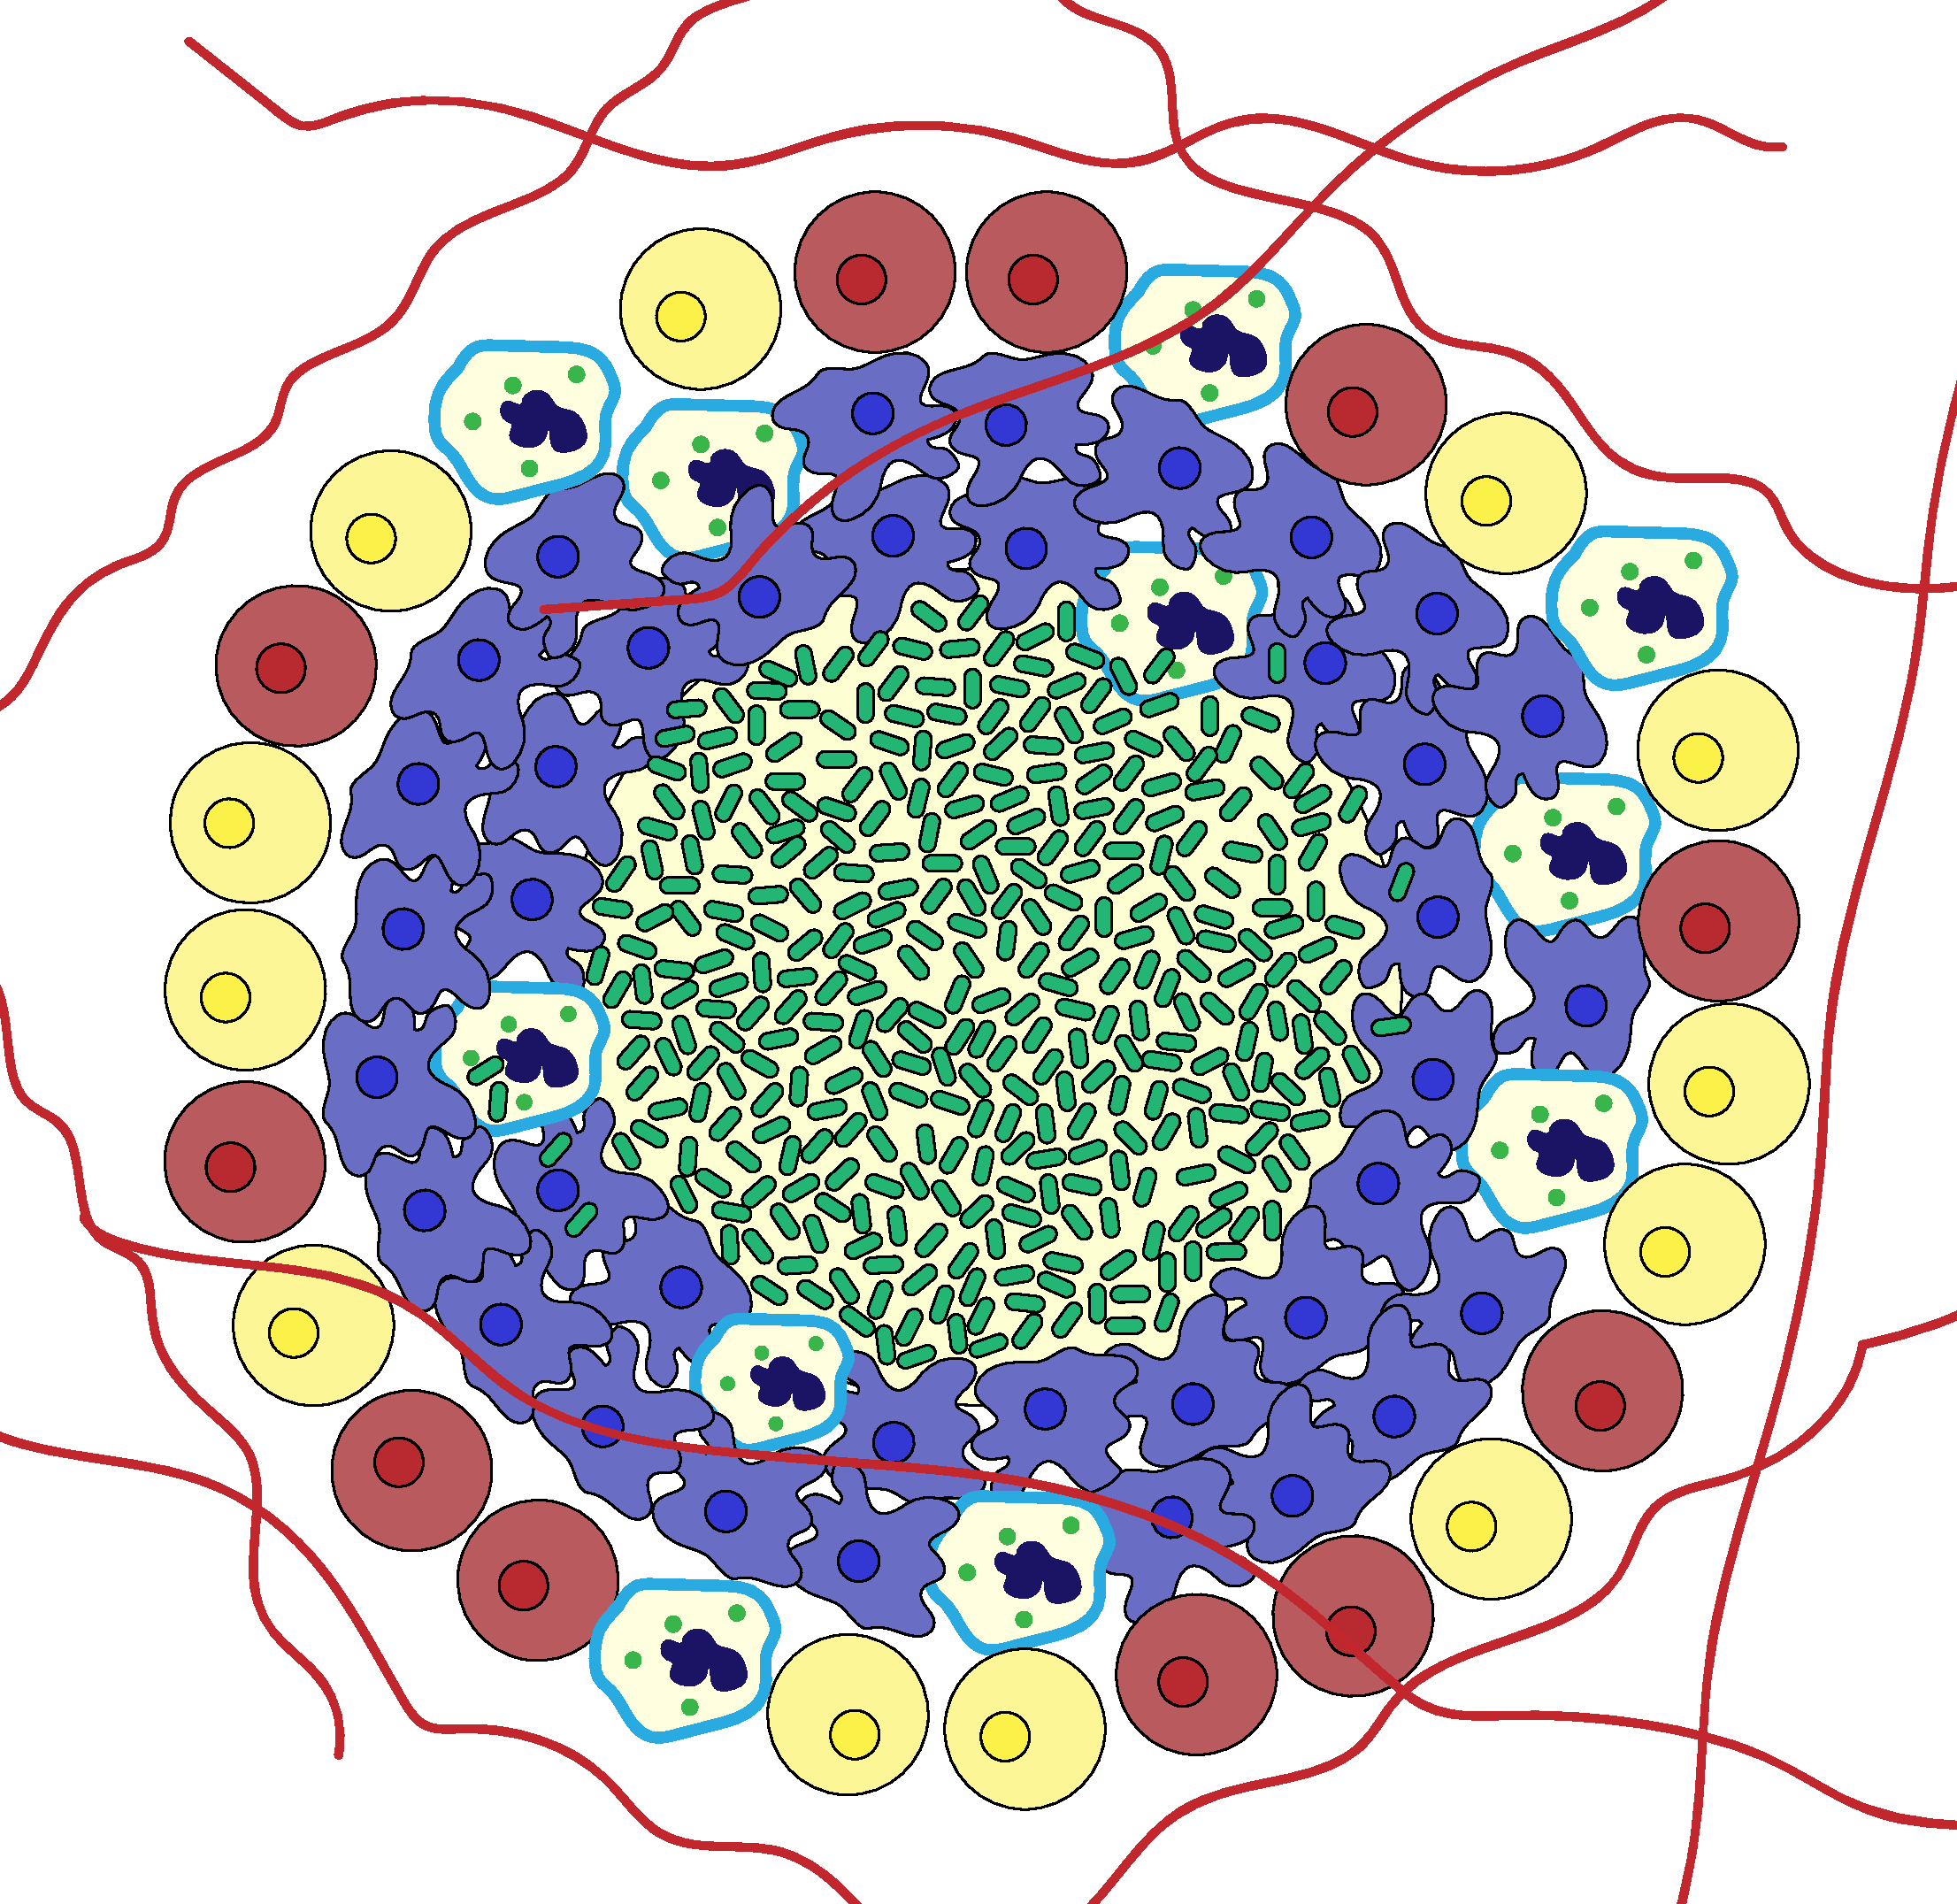
\includegraphics[height=2.5in]{images/granuloma2.pdf}
\caption[Granuloma structure schematic]{Schematic of the basic structure of a granuloma. The innermost layers are comprised of epithelioid macrophages that encase the necrotic core while outer layers are comprised of a mixture of granulocytes and lymphocytes. The whole structure is encased in a web of vasculature.}
% Provide a label so we can cross-reference it from the tex
\label{figure:granny}
\end{center}
\end{figure}

\subsubsection{Heterogeneity}

Granulomas, like the cells that comprise them, are incredibly heterogeneous structures, varying between individual granulomas within the same person and from person to person \citep{Matty2015, Lenaerts2015}. This heterogeneity is a reflection of the complex states in which macrophages can exist and their ontologies \citep{Kiss2018}. Within individual humans, the dynamics of individual granulomas showcase the diverse possible outcomes for a given infectious focus, a pattern reflected in some infection models \citep{Lin2014, Lenaerts2015}. The granuloma by the grossest histological observation contains epithelioid macrophages, motile inflammatory macrophages, multinucleated giant cells, foamy macrophages, and macrophages in various stages of various types of cell death in addition to all the other immune cell populations in the granuloma. However, even among neighboring granulomas, these relative proportions can vary widely and one can achieve effective sterilization while the other cavitates. 

This diversity within individuals in rate of progression and outcome provides a full spectrum of possibilities for each granuloma that has largely escaped our language to describe them except in sweeping intervals. Such language, including ``centroacinary\footnote{Within the alveolar space.}, perifocal, tree\hyp{}in\hyp{}bud\footnote{Bronchiolar spread leading to fluid filling the cavity, which radiologically resembles a budding tree branch \citep{Gosset2009}.}, metabolically active, exsudative\footnote{filled with circulatory fluid, but not necessarily red blood cells.}, suppurative \footnote{purulent, pus\hyp{}filled.}, miliary \footnote{Literally, millet seed\hyp{}like lesions along the lung.}, caseous, circumscribed, and fibro\hyp{}calcified\footnote{Encased in fibrotic tissue that has undergone calcification and partial ossification.}'' is but a sampling of the possible terms that pathologists can use to describe these lesions \citep{Ehlers2012}. Such striking variation can be readily seen in the images that accompany \autoref{nfatc2aAdult} and \autoref{figure:grandiv}, where the size and shape of these structures can vary widely even within an individual.

One of the many sources of this heterogeneity lies not in the genetics but in the life history of the person. Alveolar macrophages are long\hyp{}lived cells that must handle a vast diversity of insults on a daily basis and it has been shown that these insults alter their biology in a permanent fashion and likely are propagated to progeny of these mitotic cells \citep{Woodruff2005, Hodge2007, Berg2016, Glickman2016, Gonzalez2017, Duan2017}. Behaviors such as smoking are clearly inhibitory of alveolar macrophage responses and are known to exacerbate tuberculosis \citep{Hodge1996, Woodruff2005, Glickman2016}. What is not as well known is how these environmental factors alter the structure of the granuloma over the long term, especially once the granuloma has established in the interstitum and has a larger proportion of the cell mass comprised of recruited macrophages.

Even macrophages within otherwise unperturbed organs can display remarkable morphological and expressive heterogeneity \citep{Gordon2005a, Gordon2017}. This intrinsic variation from macrophage to macrophage would suggest that the outcome of tuberculosis exposure \textit{could} plausibly be determined based on which individual in a population of macrophages is first infected \citep{Verrall2014}. While this would be challenging or impossible to test experimentally, hopefully some future approach will allow this level of micro\hyp{}scale dissection of individual macrophage heterogeneity in their interactions with \textit{M. tuberculosis} \textit{in vivo} or \textit{ex vivo}. For instance, flow\hyp{}cell based approaches may allow for single macrophage\hyp{}\textit{M. tuberculosis} interactions to be modeled and subsequent single cell ATAC\hyp{}seq or RNA\hyp{}seq may identify subtle differences between macrophages that predispose them to infection or resistance within a single host. Studies from the zebrafish had displayed such within cell\hyp{}type heterogeneity clearly -- regardless of what the initial phagocytic cell is, the bacteria then subvert host responses to drive the recruitment of more permissive monocytes and macrophages, demonstrating variations in the resting capacity of these phagocytes for bacterial killing \citep{Cambier2014b}. This manipulation allows the bacteria to ``select'' their future host cells by specifically recruiting those least likely to have bactericidal capacity. This baseline heterogeneity within the host presents an exploitation schema for the bacteria that may begin at the very first encounter \citep{Ramakrishnan2013b}.

The initial events of infection remain difficult to study in most models, but insights from the zebrafish have allowed direct observation of the heterogeneous outcomes of these early events and, more importantly, potential sources of this heterogeneity which can be genetic, environmental (including the microbiome), or without clearly identifiable cause. The experimenter is burdened by entropy -- there is a great deal of intractable noise in every system and one of these sources of noise is the microbiota of the host. While no comprehensive study has yet been done on particular commensal species\footnote{A more thorough study of bacteria\hyp{}bacteria interactions during tuberculosis infection would be an intriguing new dimension to the understanding of infection. As bacteria have evolved sophisticated mechanisms of intra\hyp{}kingdom competition, it is likely the case that existing colonization with particular strains of bacteria or fungi impute resistance to tuberculosis but these have not yet been studied in any depth.} and their potentially protective or deleterious roles during tuberculosis infection, it is known that commensal species can undermine mycobacterial immune subversion by triggering TLR\hyp{}dependent sensing mechanisms that negate the shielding exercised by the infecting mycobacteria \citep{Ramakrishnan2013b, Cambier2014b}.

In the granuloma, there exists an essentially random \citep{Orme2014a} distribution of lymphocytes around the periphery of the structure. While it is clear that the innermost macrophage layers have some reasonable degree of ``organization'' as a product of their epithelial junctions with one another, other portions of the granuloma can vary substantially \citep{Cronan2016}. Even within the epithelioid layers, the macrophages remain respectably motile and are able to move throughout the granuloma to continuously remodel this structure \citep{Cronan2018}. These features likely contribute to the diverse outcomes seen within individuals in as\hyp{}yet unappreciated ways.

\section{Pattern Recognition in Innate Immunity}\label{clrs}

For over 100 years, the cells of the innate immune system were thought to be essentially blind scavengers that existed solely to pick up debris for presentation to and activation of adaptive immune responses \citep{Iwasaki2010}. How could cells saddled strictly with their somatic genotype go about ``intelligently'' identifying pathogens? The first clues came from gene homology between the cloned human IL\hyp{}1 receptor and a developmental protein from \textit{Drosophila}, Toll \citep{Lehmann1986, Heguy1992}. These similarities between IL\hyp{}1R and Toll first informed the mechanism by which IL\hyp{}1$\upalpha$/$\upbeta$ act on cells and then led to the identification of a range of proteins that shared these homologous domains required to activate NF\hyp{}$\upkappa$B \citep{Rock1998, ONeill2013}. These proteins, dubbed the Toll\hyp{}like receptors (TLRs) proved to be the foundation of the modern understanding of a very sophisticated innate immune system that, in the vast majority of cases, is solely responsible for the prevention of disease \citep{Janeway2005}. Additionally, these discoveries opened doors into the study of evolutionarily conserved mechanisms of pathogen defense, as TLRs are conserved across both \textit{Animalia} and \textit{Plantae}\footnote{This is mostly true -- plants have structurally similar proteins that recognize similar ligands, but this is thought to have arisen by convergent evolution rather than a single shared origin \citep{Johnson2003b}.} \citep{Staskawicz1995, Armant2002, Ausubel2005}. Since that time, numerous other families of receptors, known as \underline{p}attern \underline{r}ecognition \underline{r}eceptors (PRRs), have been identified that are able to detect and respond to various pathogen\hyp{}derived ligands, commonly referred to \underline{p}athogen\footnote{These are occasionally referred to as \underline{m}icrobe\hyp{}\underline{a}ssociated \underline{m}olecular \underline{p}atterns; this nomenclature successfully captures the reality that these ligands are not restricted to pathogenic species, but has not become widely used.}\hyp{}\underline{a}ssociated \underline{m}olecular \underline{p}atterns. These PAMPs serve as the foundation of the innate immune system and give it an intrinsic ability to detect and respond to threats, both from pathogens and from internal signals indicative of inflammation or damage. To varying degrees, all of these pathways have been implicated in the host response to tuberculosis, although TLR\hyp{} and CLR\hyp{}mediated responses stand out as the most well\hyp{}studied in this regard and seemingly the most prominent during infection \citep{Stamm2015}.

\subsection{Major Families of Pattern Recognition Receptors}\label{prrs}

Decades of research have revealed a number of families of pattern recognition receptors that are responsible for detecting diverse sets of widely conserved ligands from bacteria, viruses, fungi, and parasites. All of these have members that can respond, in some degree, to mycobacterial infection, making all of them relevant to the study of tuberculosis \citep{Ishikawa2017}. As alluded to previously, the Toll\hyp{}like receptor family was the first to be identified. There are 13 known TLRs in the human genome, each of which detects a number of ligands ranging from lipopolysaccharide from Gram\hyp{}negative bacteria (TLR4) and flagellin\footnote{Flagellin is the monomeric subunit used to generate bacterial flagella in motile strains that use flagella for movement.} (TLR5) to peptidoglycan\footnote{Peptidoglycan is a major component of the bacterial cell wall and is present in essentially all bacteria.} (TLR2) and RNA (TLR7) \citep{Kawai2007}. In addition to the TLR family, there are \underline{n}ucleotide \underline{o}ligomerization \underline{d}omain (NOD)\hyp{}like receptors (NLRs), \underline{r}etinoic acid\hyp{}\underline{i}nducible \underline{g}ene \underline{I} (RIG\hyp{}I)\hyp{}like receptors (RLRs), \underline{a}bsent \underline{i}n \underline{m}elanoma \underline{2}\hyp{}like receptors (ALRs), and \underline{C}\hyp{}type \underline{l}ectin \underline{r}eceptors (CLRs). All of these families can activate NF\hyp{}$\upkappa$B signaling, highlighting the central importance of this pathway in activating immunoresponsive genetic programs and executing host defense against pathogens. However, most of these receptors also engage more specific immune pathways downstream that provide them with unique responses tailored to the classes of pathogens to which they are responding.

TLR activation has long been the model for understanding the host innate immune response to pathogens. TLR activation induces a somewhat monotone response dominated by NF\hyp{}$\upkappa$B \citep{Arbibe2000, Kawai2007, Kawai2009, Brandt2013}. Most of the TLRs utilize a downstream adaptor protein, MYD88, while others (TLR3 and some TLR4 responses) utilize a different adaptor, TRIF \citep{Yamamoto2003}, to transduce signals which ultimately lead to the phosphorylation of inhibitor of nuclear factor kappa B (I\hyp{}$\upkappa$B) by the I$\upkappa$B kinase (IKK), which releases NF\hyp{}$\upkappa$B for translocation into the nucleus \citep{Wright1990, Kawai1999, Triantafilou2002, Yamamoto2003, Akira2004, Takeda2004, Kawasaki2014}. This transcription factor family is often viewed in a somewhat monolithic manner, but is comprised of five independent transcription factors (NF\hyp{}$\upkappa$B1, NF\hyp{}$\upkappa$B2, RelA, RelB, and c\hyp{}Rel) that generally act as heterodimers with one another; this raises the potential for subtle and as yet undescribed levels of regulatory complexity\footnote{Principally, there are 20 different permutations of these proteins just on their own and not accounting for the complex additional layers of possible regulation with additional binding partners.} based on the active heterodimers in different contexts \citep{Rice1992, Baeuerle1994, Finco1995, Oeckinghaus2009, Ghosh2012, Liu2017a, Albensi2019}. To date, little has been done to fully characterize these distinctions, although some work has found different transcription factor bindings sites to be preferentially bound by some dimers and not others \citep{Siggers2011, Ramsey2019, Florio2022}. Nonetheless, NF\hyp{}$\upkappa$B activation writ large is able to activate transcription of a full spectrum of cytokines and chemokines, including IL\hyp{}1$\upbeta$, IL\hyp{}6, IL\hyp{}12, IL\hyp{}17, IFN\hyp{}$\upalpha$/$\upbeta$, TNF\hyp{}$\upalpha$, and IFN\hyp{}$\upgamma$ \citep{Pahl1999, Gilmore2006, Liu2017a}. This robust pro\hyp{}inflammatory response is essential for effective clearance of many pathogens and also increases the resistance of surrounding tissue to further infection by intracellular pathogens. As the TLRs can recognize such a diverse array of ligands, this makes them a critical inducer of potent host\hyp{}protective responses through the induction of microbicidal pathways and recruitment of additional immune cells \citep{Kawai2007, Kawasaki2014}. 

NLRs are conserved across metazoans and detect cytosolic PAMPs to defend against intracellular pathogens \citep{Martinon2005, Creagh2006, Clarke2014, Motta2015}. NLRs, like TLRs, activate NF\hyp{}$\upkappa$B, but can also activate mitogen\hyp{}activated protein kinase (MAPK) signaling, including p38 and JNK \citep{Shaw2008, Franchi2009, Zhong2013, Saxena2014, Platnich2019, Velloso2019}. NLRs detect a range of primarily bacterial ligands, including gamma\hyp{}D\hyp{}glutamyl\hyp{}meso\hyp{}diaminopimelic acid (iE\hyp{}DAP) from Gram\hyp{}negative bacteria, muramyl dipeptide from pan\hyp{}bacterial peptidoglycan, \textit{Legionella} flagellin, and bacterial RNA \citep{Franchi2009, Zhong2013, Saxena2014}. NLRs initiate the formation of inflammasomes: large, cytosolic, punctate structures that process pro\hyp{}IL\hyp{}1$\upbeta$ and pro\hyp{}IL\hyp{}18 for secretion and paracrine signaling. Within the responding cell itself, however, the combination of MAPK and NF\hyp{}$\upkappa$B signaling provides a different signaling tone to that induced by TLRs. MAPKs are known to induce the expression of IL\hyp{}1$\upalpha$/$\upbeta$, IL\hyp{}10, IL\hyp{}12, and TNF\hyp{}$\upalpha$ \citep{Dong2002, Arthur2013, SoaresSilva2016}, which are potent immunomodulators, with TNF\hyp{}$\upalpha$ inducing cell death and inflammation while IL\hyp{}10 is a potent anti\hyp{}inflammatory chemokine \citep{Couper2008, Ouyang2011, SoaresSilva2016}. Work remains to be done to more thoroughly define the specific MAPK\hyp{}dependent responses downstream of NLR activation, which may inform more targeted approaches to immunotherapy in the context of infection.

RLRs are an additional class of cytosolic sensors, most commonly implicated in the antiviral immune response as they detect aberrant nucleic acids, usually those with abnormal features that would not typically be found in eukaryotic cells, including double\hyp{}stranded RNA and uncapped single\hyp{}stranded RNA of varying lengths \citep{Kawai2010, Loo2011, Rehwinkel2020, Jia2021}. The RLR family is composed of RIG\hyp{}I itself as well as MDA5; these have distinct affinity for different ligands, but both ultimately activate IRF3/7 to induce transcription of IFN\hyp{}$\upalpha$/$\upbeta$, classic type I interferons that activate autocrine and paracrine JAK/STAT signaling to promote antiviral responses in neighboring tissues \citep{Loo2011}. These responses are notable in the history of hepatitis C treatment, as the previous standard of care treatment for hepatitis C was treatment with IFN\hyp{}$\upalpha$, which facilitated viral clearance in many cases \citep{Rong2010}. Interestingly, RIG\hyp{}I signaling is also able to mediate some immune responses against \textit{M. tuberculosis} and drives the production of IFN\hyp{}$\upbeta$ through MAVS to exacerbate pathology; \textit{Mavs} mutant mice had dramatically improved survival after challenge \citep{Cheng2018}. The precise ligands for MAVS produced by \textit{M. tuberculosis} remain unknown, but may involve outer membrane vesicles, which can carry RNA cargo \citep{PradosRosales2011, Brown2015, Tsatsaronis2018, DaurosSingorenko2018, Gupta2018, Chiplunkar2019}.

ALRs are the newest addition to the class of PRRs and serve to detect cytosolic DNA -- a potent signal of some sort of pathogenic invasion, either by DNA viruses or some bacteria, or cellular damage. These direct sensors of cytosolic DNA appear to be largely redundant with the existing cGAS pathway as both of these pathways activate STING, which induces the interferon response cascade \citep{Gray2016}. However, an alternative hypothesis suggested that ALRs \textit{antagonize} the interferon response by inhibiting cGAS\hyp{}mediated activation of STING \citep{Nakaya2017}. These genes are important for promoting the pathogenesis of tuberculosis, as in the absence of IFI16 and the effector IRF3, \textit{M. tuberculosis} is attenuated for growth in a mouse model \citep{Manzanillo2012}. It is hypothesized, although seemingly untested, that each of the 13 ALR genes (in mice) have distinct families of targets and exerts these modulating effects in distinct contexts in cooperation and antagonism with STING \citep{Nakaya2017}. As this pathway is relatively new to study, there is still a great deal to be learned about how it mediates type I interferon responses and how those interact with engagement of other PRR signaling pathways. However, early studies have already begun to identify consequences of misregulation of these genes, including in the development of autoimmunity \citep{Caneparo2018}.

\subsection{LPS as a Model Molecular Pattern}\label{lps}

Lipopolysaccharide (LPS) from Gram\hyp{}negative bacteria has long been the model for understanding ligand\hyp{}receptor interactions and signal transduction in the context of PAMP\hyp{}PRR pairs. On the cell surface, LPS is detected by a complex of CD14, MD2, and TLR4, making it a rather unusual mechanism of detection in comparison to other TLRs, which can either independently detect ligands or act in heterodimers with other members of the TLR family. This complex coordinates the activation of MYD88 and TRIF, which activate NF\hyp{}$\upkappa$B signaling as previously described \citep{Beutler2000, Miller2005}. For intracellular LPS, which might be encountered in the context of a cytosolic bacterial infection, detection by Caspase\hyp{}11 mediates the formation of inflammasomes to process IL\hyp{}1$\upbeta$ and IL\hyp{}18 to defend against these intracellular Gram\hyp{}negative bacterial pathogens \citep{Wright1990, Kawai1999, Triantafilou2002, Kayagaki2013, Shi2014, Rathinam2019, Vasudevan2022}. LPS\hyp{}TLR4 interactions mediate key aspects of sepsis -- a systemic inflammatory disorder set on by infection -- as well as normal immune responses \citep{Freudenberg2008}.

TLR4 was the first of the TLR family to be characterized and remains the most thoroughly studied \citep{Lu2008}. The ostensible ligand (albeit indirectly via CD14) for TLR4 was identified as LPS, a highly conserved pattern on the outer leaflet of the outer membrane of Gram\hyp{}negative bacteria \citep{Wright1990, Guha2001, Kayagaki2013, Shi2014}. LPS, while once again often stated as a monolithic entity, is in fact a whole family of diverse lipoglycans that vary widely in saccharide antigen and lipid composition, which has become an active area of study \citep{Raetz2007, Maldonado2016, Steimle2016, SenGupta2016, Kutsch2020, Dickinson2022}. LPS, as the name suggests, is comprised of a lipid moiety that docks into the outer leaflet of the outer membrane of Gram negative bacteria and is connected to a series of well\hyp{}defined and highly diverse glycans in different physical locations along the molecule; the outermost of these is a the O\hyp{}antigen, which in some species can antagonize adaptive immune responses \citep{DominguezMedina2020}. In addition to the highly variable O\hyp{}antigen, other regions within the molecule can vary within a single bacterium, over time, and across species.

The precise composition of the lipid tails of LPS alters its ability to bind TLR4 and induce inflammatory responses. Pathogenic species of Gram\hyp{}negative bacteria tend to have six (6) lipid tails on LPS that activate TLR4 while commensal or environmental species have five (5) or fewer lipid tails that do not activate TLR4\footnote{For instance, the oral opportunistic pathogen \textit{Porphyromonas gingivalis} produces a tetraacylated LPS that actually inhibits TLR4 activation by hexaacylated LPS from \textit{Escherichia coli} \citep{Darveau2004, Zhang2008a, Herath2013}.} \citep{Dixon2005, Ueda2010, Lebeer2010, Gyorfy2013, Tan2015, Steimle2016, Simpson2019}. Precisely why and how these differences have emerged and evolutionary rationales for the failure of pathogenic species to adopt immune evading tetra\hyp{} or penta\hyp{}acyl LPS and instead adopt hepta\hyp{}acyl LPS during infection \citep{SenGupta2016} is the subject of ongoing work, but it seems undoubted that some aspects of the TLR\hyp{}dependent response pathway must offer benefit to the bacteria and provide an avenue of bacterial subversion against the host immune response, although this remains understudied in non\hyp{}tuberculous bacterial infections \citep{Park2013, McGuire2015}.

The ability for variations of a single structure to modulate such diverse host immune responses establishes a model for pathogens to intricately manipulate the features of these widely shared and physiologically essential patterns to alter immune response capacity and, potentially, drive bacterially\hyp{}beneficial responses through perversion of the ``intended'' role of these host receptors. The molecule of interest for my purposes, TDM, is comparatively less studied in the context of host immunity, driving some uncertainty around the direct mediators of this response. Additionally, the specific presentation and conformation of TDM seems to impact the immune response generated to this ligand. \textit{In vitro}, TDM has been demonstrated to adopt different conformational states based on surface composition (for instance, at the air\hyp{}water interface) and geometry, although the \textit{in vivo} relevance of these different states is contentious \citep{Behling1993, Hunter2006b}. While this will be detailed in \autoref{tdmreceptor}, the major receptors known to detect TDM are within the C\hyp{}type lectin receptor family and are known as MINCLE and MCL.

\subsection{Signaling Mechanisms Downstream of C\hyp{}Type Lectin Receptors}\label{clrsig}

While TLR activation \textit{per se} is a rather monotonal response that is predominantly driven by NF\hyp{}$\upkappa$B, CLRs terminate in at least two known downstream signaling pathways. In addition to NF\hyp{}$\upkappa$B (via a pathway to be discussed shortly), they are capable of activating the \underline{n}uclear \underline{f}actor of \underline{a}ctivated \underline{T} cells (NF\hyp{}AT or NFAT) pathway \citep{Goodridge2007, Dambuza2015}. This ability to activate multiple layers of transcriptional regulation either at the same time or under different contexts (length of time, strength of agonism, particular ligand) offers CLRs a powerful additional mechanism of modulating the tone of the immunological response in response to particular insults \citep{Brown2018}. 

CLRs are a diverse class of pattern recognition receptors that are defined by their use of divalent calcium (Ca\textsuperscript{2+}) to coordinate the binding of carbohydrate patterns \citep{Hosoi1998, Dodd2001}, generally segregated into two major classes: QPD (glutamine\hyp{}proline\hyp{}aspartate) motif lectins, which bind galactose\hyp{}containing sugars, and EPN (glutamate\hyp{}proline\hyp{}asparagine) motif lectins, which bind mannose\hyp{} or glucose\hyp{}containing sugars \citep{Holtet1997, Zelensky2005, Furukawa2013, Alenton2017}. QPD\hyp{}containing C\hyp{}type lectins are, in general soluble or secreted proteins and include the likes of human tetranectin (CLEC3B), an extracellular matrix\hyp{}interacting protein, and herring antifreeze protein, which mediates the breakdown of ice crystals in the blood of cold\hyp{}water fish \citep{Ewart1993, Nielsen1997, Ewart1998, Graversen1998, Liu2007}. 

These receptors are critical mediators of antibacterial, antiviral, and antifungal immunity and have evolved to encompass a vast range of different receptors with unique ligand specificities and expression patterns \citep{Hoving2014, Tang2018}. CLRs are known to respond primarily to these carbohydrate\hyp{}linked ligands via their lectin domains \citep{Dodd2001, McGreal2005}. Many biomolecules are sugar\hyp{}modified, including those from bacteria, fungi, viruses, archaea, and eukaryotes (both self and pathogens) \citep{Rudd2001, Ohtsubo2006}. This allows CLRs to be a major pathway for the response to host\hyp{}derived \underline{d}amage\hyp{}\underline{a}ssociated \underline{m}olecular \underline{p}atterns (DAMPs) as well as PAMPs \citep{GarciaVallejo2009}. By contrast, EPN C\hyp{}type lectins play a diverse set of roles and many are the classical members of the CLR family, with many being transmembrane receptors \citep{Sancho2012}. Most notable among these CLRs is DECTIN\hyp{}1, the archetypal member of the family which has long been studied for its roles in antifungal immunity, but has now been discovered to have a diverse set of roles in other conditions, including responses to bacterial pathogens (including mycobacteria) and in autoimmunity \citep{Brown2002, Brown2003, Brown2006, Yadav2006, Schorey2008, Reid2009, Drummond2011b, Wagener2018, Deerhake2021}. 

DECTIN\hyp{}1 has provided the scientific foundation of much of the knowledge we have about the mechanisms of signaling downstream of CLR activation. DECTIN\hyp{}1\hyp{}mediated signaling responses are known to be protective against fungal infections, making this a centerpiece of defense against common fungal pathogens, including \textit{Malassezia} and \textit{Candida}\footnote{Interestingly, this role for C\hyp{}type lectin receptors in defending against fungi is not ubiquitous and it seems that \textit{Cryptococcus} has evolved mechanisms to avoid detection by most or all of those present in the human host \citep{Walsh2017}. These masking mechanisms can be perturbed by changes in the cell wall composition of the fungi, suggesting that this is an adaptive mechanism of protection for the pathogen \citep{Esher2018}.} \citep{Shiokawa2017}. Although not the focus of the present work, DECTIN\hyp{}1 also has a number of important roles in antimycobacterial defense, which established the importance for this class of C\hyp{}type lectin receptors in tuberculosis \citep{Yadav2006}. DECTIN\hyp{}1 is a single\hyp{}pass transmembrane receptor that uses a large C\hyp{}type lectin domain to engage with various ligands, most notably $\upbeta$\hyp{}glucans, to stimulate responses in myeloid cells \citep{Brown2007}. DECTIN\hyp{}1 itself possesses an intracellular YxxL/I (hemITAM) motif that is then phosphorylated by an adaptor kinase, spleen tyrosine kinase\footnote{SYK itself has many important roles in macrophage and B cell biology, but to spare the distraction, see \citet{Mocsai2010} for a nice review of these roles. SYK is critical for phagosomal\hyp{}lysosomal fusion and other roles within macrophages \citep{Tabata2020}. This also makes SYK a poor genetic target as disruption is embryonic lethal in mice \citep{Yanagi2001}.} (SYK) \citep{Kerrigan2011, Getahun2015, Bauer2017}. It has been shown that stabilization of SYK facilitates stronger immunological responses and fosters protection against fungal infections; cells actively degrade this kinase to limit inflammation, sometimes to the detriment of effective immune clearance \citep{Sohn2003, Wirnsberger2016, Zhu2016}. The ITAM motif is critical for the binding and activation of downstream processes from a range of tyrosine kinase\hyp{}dependent receptors, including B cell receptor activation \citep{Monroe2006, Bauer2017}. This sets off a complex series of signaling events that activate CARD9, ASC, and/or PLC$\upgamma$2, eventually resulting in NF\hyp{}$\upkappa$B activation in the former two instances and NFAT activation in the latter \citep{Geijtenbeek2009, Drummond2013}. For DECTIN\hyp{}1 specifically notable roles have been defined for both of these branches in this signaling pathway but much less is known about these pathways downstream of other, related receptors.

\subsubsection{CARD9}\label{clr:card9}

CARD9\hyp{}mediated signaling has long been considered to be the dominant modality of signaling downstream of C\hyp{}type lectin receptors and is important for transcriptional responses to and defense against many intracellular pathogens \citep{Hsu2007, Hara2007}. This pathway was identified as a critical mediator of TLR\hyp{}independent antifungal immunity through DECTIN\hyp{}1, establishing the prototype for C\hyp{}type lectin signaling responses \citep{Gross2006}. Human CARD9 deficiencies have a very specific susceptibility to fungal infections, but interestingly not other types of infections \citep{Drummond2016, Drummond2018}.

One of the major focuses has been on the importance of CARD9\hyp{}BCL10\hyp{}MALT1 (CBM) signalosomes as a unique consequence of CLR agonism \citep{Marakalala2010, Drummond2011a, Drummond2016, Marakalala2017, Drummond2018}. Despite utilizing a method of activation that has more in common with B cell receptor activation than TLRs \citep{Monroe2006}, the functional downstream consequence is the same: nuclear translocation of NF\hyp{}$\upkappa$B through IKK and associated induction of immune response genes including IL\hyp{}2\footnote{While all of these genes are confusing from most perspectives, this one is extremely confusing and requires a bit of gymnastics to come to -- why would it be assumed that NF\hyp{}$\upkappa$B signaling is mediating IL\hyp{}2 expression in the context of the body of literature stating that NFAT is the almost exclusive regulator of IL\hyp{}2 with no affirmative evidence of that being the case?}, IL\hyp{}10, TNF\hyp{}$\upalpha$, and more \citep{Sancho2012}. Furthermore, the evidence is extremely strong that CBM\hyp{}dependent signaling is critical for the response to a variety of fungal pathogens and that these generally type I responses are a potent defense against infection \citep{Willment2008, Hardison2012, Drummond2018}. Despite this, early studies found that unprimed macrophages do not utilize the CBM signalosome and require priming in order to active CARD9\hyp{}dependent transcriptional responses \citep{Goodridge2009}. These variations in the ability for DECTIN\hyp{}1 to induce CARD9 activation may be useful in discriminating between different types of downstream responses; that study specifically found that bone\hyp{}marrow derived macrophages exhibited DECTIN\hyp{}1 responses that were essentially independent of CARD9 while dendritic cells promoted CARD9\hyp{}dependent signaling. The responses downstream of C\hyp{}type lectin activation through CARD9 tend to activate T\textsubscript{H}1 and T\textsubscript{H}17 responses, which are important for effective fungal control and defense against mycobacterial infections \citep{Zanoni2005, Zenaro2009, Drummond2011a, Lyadova2015}. However, newer datasets have provided evidence of a range of genes that depend on CLR activation but are CARD9\hyp{}independent \citep{Deerhake2021}. Some of these genes are likely to be NFAT\hyp{}dependent while others may be activated by as\hyp{}yet unidentified pathway or through more indirect mechanisms.

Specifically in tuberculosis immunity, CARD9 is important for limiting bacterial growth; in its absence, mice develop severe pneumonia and rapidly succumb to infection. Several different C\hyp{}type lectin receptors can activate CARD9, so mutation of this adaptor protein compromises signaling through several distinct receptors that recognize a range of ligands \citep{Wagener2018}. Some of these effects may be mediated by loss of DECTIN\hyp{}1\hyp{}dependent responses, but much is likely to be mediated by other receptors, as will be discussed in \autoref{tdmreceptor} \citep{Marakalala2010, Marakalala2017}. CARD9 is not only essential for transcriptional responses downstream of C\hyp{}type lectin receptors, it is also required for the transcriptional induction of MINCLE downstream of MCL. This provides a priming step that depends on CARD9 and then feeds\hyp{}forward with additional CARD9\hyp{}dependent MINCLE expression for the duration of agonism \citep{Zhao2014}.

This pathway also has known roles in exacerbating autoimmunity. A definitive study on the matter by \citet{Deerhake2021} demonstrated that Card9\footnote{Throughout this document, whenever I am synthesizing data from different sources or speaking of a pathway in the abstract, I will typically use human gene nomenclature \citep{Tweedie2021}, however, when discussing particular studies in depth, I will adopt the nomenclature of the model organism used (in this case, the mouse). I hope to minimize any confusion on this topic by using species\hyp{}specific nomenclature only sparingly and when relevant to the topic at hand.} activation during experimental autoimmune encephalomyelitis drove pathology despite the overall protective effects of Dectin\hyp{}1 activity. This study generated a comprehensive dataset of the Card9\hyp{}dependent signaling events in myeloid cells after exposure to the Dectin\hyp{}1 agonist curdlan. This will provide a great deal of value to future experimenters attempting to isolate the contributions of distinct signaling pathways to an observed C\hyp{}type lectin\hyp{}dependent phenotype.

As will be discussed more exhaustively in \autoref{tams}, macrophages associated with tumors exert particular levels of regulation over the biology of the tumor itself. In this context, CARD9 is able to be activated by tumors to drive increased tumor metastasis \citep{Yang2014b}. In the context of wound healing, CARD9 is required for effective closure; this offers a different side to CARD9 signaling, which is often viewed as strictly inflammatory, but is evidently important for wound healing processes as well although the mechanisms remain largely unknown \citep{Kanno2017}.

\subsubsection{Inflammasomes}\label{clr:asc}

CLR activation also results in the activation of ASC\hyp{}dependent canonical inflammasomes, which process pro\hyp{}IL\hyp{}1$\upbeta$ and pro\hyp{}IL\hyp{}18 for secretion and paracrine and autocrine signaling \citep{Gross2011} and play critical roles during both development and pathogen responses \citep{Tyrkalska2019}. This occurs through the formation of an intracellular signaling complex with many distinct subunits that, together, mediate the activation of inflammatory programs and pyroptosis \citep{Pandey2021}. These IL\hyp{}1$\upbeta$\hyp{} and IL\hyp{}18\hyp{}dependent responses depend on the previously mentioned IL\hyp{}1R which utilizes MYD88 to drive signaling, linking it into common sets of signals that are induced by TLR activation. This single pathway thus plays a critical and somewhat circular role in various facets of the host response downstream of TLR activation, which unifies the response tone while potentially restricting response diversity; while TLRs are somewhat broad in their expression pattern, the induction of IL\hyp{}1$\upbeta$ secretion activates all neighboring cells that express IL\hyp{}1R, which is practically ubiquitous in environment\hyp{}facing tissues \citep{Deyerle1992, Malik2018}. This makes this pathway extremely powerful for increasing the local inflammatory tone to block the replication and spread of (especially intracellular) pathogens, but subject to a complex set of subversive mechanisms utilized by bacteria, fungi, and viruses \citep{Poeck2010, MacMicking2012, Tavares2015, Wein2022}. Comparatively less work has been done to characterize the activating mechanisms induced by CLRs that result in inflammasome formation, but this could serve as an exacerbatory mechanism to heighten inflammation in response to particular classes of signal. Notably, LPS (the canonical TLR4 ligand) is also capable of activating inflammasomes, albeit by an entirely distinct Caspase\hyp{}11\hyp{}dependent mechanism \citep{Hagar2013, Pilla2014, Vanaja2016, Finethy2020}.

Inflammasome activation has many described roles in the control of mycobacterial infections and is actively manipulated by the bacteria, suggesting that C\hyp{}type lectin mediated activation of this pathway may play a role in host defense against mycobacteria as it does against fungi \citep{Hardison2012, Wassermann2015}. Knockout of the mediator caspases results in increased bacterial burden in a strictly innate immune context \citep{Kenyon2017}. However, it has been demonstrated that \textit{M. tuberculosis} actively blocks activation of the inflammasome, suggesting that this pathway may be of variable efficacy in defense against mycobacteria, or that inflammasome\hyp{}mediated activation of gasdermin D is a more important mediator of these effects than is pro\hyp{}IL\hyp{}1$\upbeta$ processing \citep{Master2008, Qu2020}. Yet another plausible alternative incorporates non\hyp{}canonical or inflammasome\hyp{}independent functions of ASC, as ASC knockout mice demonstrate increased susceptibility to infection while NLRP3 and Caspase\hyp{}1 are both dispensable for protection \citep{McElvaniaTekippe2010}. There are also a number of tools that can be utilized to study this process, including a fluorescent ASC knock\hyp{}in line that report inflammasome activation through visible formation of the characteristic cytosolic specks \citep{Kuri2017}. Such controversy within the field makes this a prime area for future clarifying study although it may be a technical challenge to disentangle some of these complex factors. Despite known role for CLR signaling in activating the inflammasome, the primary activation mechanism in mycobacterial infection is presumed to be via plasma membrane damage, although this does not rule out contributions from other pathways \citep{Beckwith2020}.

\subsubsection{NFAT}\label{clr:nfat}

Lastly, CLRs can activate NFAT signaling, which is a signaling pathway common across developmental processes but is thought to be a unique consequence of CLR agonism in respect to PRR activation and, as such, is often used as a reporter for CLR activity \citep{Aramburu1998, Chow1999, Hooijberg2000, Jauliac2002, Wilkins2004, Goodridge2007, Fuller2007, Goodridge2008, Zhao2014, HannantaAnan2016, Bendickova2020}. Despite the relative uniqueness of this pathway to CLRs, comparatively less work has been done to characterize it vis\hyp{}\`{a}\hyp{}vis the CARD9\hyp{}NF\hyp{}$\upkappa$B pathway \citep{Goodridge2007, Goodridge2009, Deerhake2021}. This pathway can induce the expression of EGR2, EGR3, COX2, IL\hyp{}2, IL\hyp{}10, and others, which is a more anti\hyp{}inflammatory or immunoregulatory set of signals than the heavily type I signals induced by NF\hyp{}$\upkappa$B (IL\hyp{}1, IFN\hyp{}$\upgamma$, etc.) \citep{Saraiva2010}. The interplay between these divergent signaling consequences is poorly understood, but is likely important in determining the overall tone and kinetics of the response to infection. This pathway will be given a much more extensive dissection in \autoref{NFAT}, but suffice to say that the consequences of this pathway's activity downstream of CLR activation are critical but poorly understood mediators of the overall response in tandem with NF\hyp{}$\upkappa$B activation.

\subsubsection{Phagocytosis}

One of the key integration mechanisms between C\hyp{}type lectin receptors and NFAT pathway activation is the contribution that C\hyp{}type lectins make to myeloid cell phagocytosis. These cells are widespread phagocytic receptors and are critical for the uptake of fungi \citep{Robinson2006}. Could this be the case during mycobacterial infections? Seemingly so. The mannose receptor (CD206) is thought to be a major uptake receptor for mycobacteria, as ectopic expression drives the internalization of mycobacteria in other cell types \citep{Schlesinger1993}. While this is somewhat redundant with other mechanisms of uptake, this suggests a fundamental role for C\hyp{}type lectins in driving mycobacterial phagocytosis \citep{Ernst1998}. One of the central consequences of the phagocytosis of any particle is the activation of the NFAT signaling pathway -- tying this pathway intimately to the response to diverse infections and activation of adaptive immunity \citep{Khameneh2017}. Given that NFAT signaling is at the root of these earliest host interactions with mycobacteria, it is bizarre that this pathways has been comparatively neglected for so long. It is my hope that the discussion provided here and the resulted presented later on will spur further investigation into the contributions of calcineurin\hyp{}NFAT signaling to the earliest events of innate immunity \citep{Jayachandran2007, Jayachandran2008}. 

An excellent study by \citet{Goodridge2011} found that the activation of DECTIN\hyp{}1 was dependent upon binding immobilized ligand. Soluble $\upbeta$\hyp{}glucan particles were unable to activate DECTIN\hyp{}1 while those same particles immobilized on plastic were sufficient to do so, providing a model wherein C\hyp{}type lectin receptors can discriminate between happenstance binding of soluble ligands and direct microbial recognition to only induce phagocytosis when bound by a sufficiently large particle \citep{Elder2017}. This prevents microbes from shedding small decoy ligands to distract the innate immune system and induce aberrant and energetically costly phagocytosis. This phagocytosis in intimately linked to the activation of NFAT, where internalization of particles through phagocytic receptors (primarily C\hyp{}type lectins) facilitates increased signaling activity \citep{Fric2014}. Whether this is the case for every conceivable ligand is unknown and unlikely, but it, at minimum, offers yet another mechanism for host detection and potential microbial subversion.

These phagocytic activities require an intricate (and often physical) association between the inducing receptor with calcium ion channels, calmodulin, calcineurin, and mTOR. It has been found that STIM1 physically links phagosomes to the endoplasmic reticulum to enhance phagocytosis; this release of calcium via STIM1 is then able to activate NFAT to drive further transcriptional responses meant to address the contents of the phagocytic vesicle, to varying degrees of success \citep{Nunes2012}. The contributions of NFAT in controlling intracellular mycobacterial growth is wholly unknown but is presumably subject to extensive modulation by the infecting bacteria. Such limitation of NFAT responses within the macrophage while it is infected may be a compelling explanation for the extracellular exposure\hyp{}specific responses observed in \autoref{extracellular}.

\subsection{C\hyp{}Type Lectins in Tuberculosis}

In addition to DECTIN\hyp{}1, there are a number of other C\hyp{}type lectin receptors that have come under study for their contributions to host immunity. DECTIN\hyp{}1 itself is thought to bind to mycobacteria, although the ligand remains unknown and DECTIN\hyp{}1 is dispensable for effective antimycobacterial responses \citep{Yadav2006, Rothfuchs2007, Schorey2008, Marakalala2011}. One of these other receptors largely predates acknowledgement of C\hyp{}type lectins as a major pattern recognition signaling pathway but is critical for bacterial uptake. As previously mentioned, the mannose receptor is a major contributor to mycobacterial phagocytosis in a manner partially redundant with complement opsonization and uptake \citep{Schlesinger1993, Kang1998b}. However, this mode of uptake does not induce lysosomal fusion and is thus a pro\hyp{}bacterial mode of cell entry, allowing access to permissive host environments and evading bactericidal immune cells \citep{AstarieDequeker1999, Goyal2016, Rajaram2017}. 

DC\hyp{}SIGN was the first C\hyp{}type lectin receptor to have described roles in host protection against \textit{M. tuberculosis}. It was initially described as the major receptor for mycobacteria on the surface of dendritic cells, although it is now known to also be expressed by macrophages, especially alveolar macrophages \citep{Geijtenbeek2002, Tailleux2003, Tailleux2005}. The general consensus was that DC\hyp{}SIGN expression was a mechanism for host subversion by mycobacteria, but that does not adequately explain the function of DC\hyp{}SIGN \textit{in primo loco} \citep{vanKooyk2003}, especially as the mycobacteria specifically target DC\hyp{}SIGN to inhibit host immunity \citep{Geijtenbeek2003}. In this context, binding of \textit{M. tuberculosis} mannose\hyp{}capped lipoarabinomannan (ManLAM) \citep{Maeda2003, Koppel2004, Pitarque2005} to DC\hyp{}SIGN induced IL\hyp{}6, IL\hyp{}10 and IL\hyp{}12 expression by dendritic cells; similar effects were seen with binding of HIV\hyp{}1, \textit{Helicobacter pylori}, and \textit{Aspergillus}, making DC\hyp{}SIGN a rather promiscuous receptor of pan\hyp{}kingdom ligands ranging from bacteria to fungi to viruses \citep{SerranoGomez2005, Gringhuis2009, denDunnen2009}. Interestingly, this gene is all but impossible to study in the murine model because mice have no fewer than eight DC\hyp{}SIGN duplicates, evidence of the evolutionary pressures likely to have necessitated such diversification of function, which may be common to C\hyp{}type lectin receptors more generally \citep{Tanne2009, GarciaVallejo2013}.

There are other C\hyp{}type lectin receptors that engage distinct aspects of host immunity to tuberculosis \citep{Mishra2017a}. DECTIN\hyp{}2 has been shown to detect mannose\hyp{}capped lipoarabinomannans and induce the expression of a by now familiar cast of cytokines -- IL\hyp{}2, IL\hyp{}6, IL\hyp{}10, and TNF\hyp{}$\upalpha$. This ligand is another component of the mycobacterial cell wall and is likely to be exposed after bacterial killing or other loss of cell wall integrity, so is unlikely to be a phagocytic receptor for mycobacteria, but may be an important mediator of bystander cell activation \citep{Marakalala2017}. All of these receptors have major downstream pathways that run through CARD9\hyp{}NF\hyp{}$\upkappa$B, which has been shown to be important for mycobacterial control and limitation of inflammatory responses through IL\hyp{}10 \citep{Dorhoi2010}.

Two additional members of the EPN\hyp{}containing superfamily of CLRs are MCL and MINCLE\footnote{Interestingly, engagement of MINCLE by fungi suppresses the protective DECTIN\hyp{}1\hyp{}mediated responses. How these receptors can be manipulated by pathogens to be either active or repressive is an interesting biochemical and biophysical question that has yet to be fully addressed \citep{Wevers2014}.}. MCL, originally dubbed DECTIN\hyp{}3\footnote{And for historical reasons, is still occasionally called this in the modern literature.}, is expressed by myeloid cells at baseline and is a comparatively desensitized receptor with low affinity for its primary known ligand, TDM \citep{Zhu2013, Miyake2013, Zhao2014}. MINCLE, on the other hand, is tightly regulated and only induced after cellular priming by some other stimulus, including MCL activation \citep{Wells2008, Patin2017a}. MINCLE has much higher affinity for TDM and, seemingly, a broader range of agonizing ligands, although the latter discrepancy may be a result of historical scientific focus rather than authentic biological difference \citep{Richardson2014, Feinberg2016, Hansen2019}.

\subsection{The TDM Receptor}\label{tdmreceptor}

TDM exerts similarly diverse functions as LPS and is also detected by host pattern recognitions receptors (PRRs) including TLR2 -- another member of the Toll\hyp{}like receptor family -- and two C\hyp{}type lectin receptors (CLRs), MINCLE and MCL. As discussed in \autoref{cellwall} and \autoref{tdm}, TDM is a structurally essential component of mycobacteria; the absence of TDM renders the bacteria susceptible to killing by immunological, chemical, and environmental stressors \citep{Rao2005, KanSutton2009, Moliva2019}. In addition to the important structural aspects of TDM, it also possesses a number of chemical and biological functions in interactions between pathogenic mycobacteria and their hosts.

Chemically, TDM is radically different from nearly any other biomolecule that an organism is likely to encounter. Comprised of a trehalose head group -- an unusual di\hyp{}glucose that is never synthesized by animals \citep{Elbein2003} -- attached to profoundly hydrophobic, extremely long, and diversely modified branched fatty acid tails, TDM is directly cytotoxic to cells through disruption of plasma membrane integrity (\autoref{figure:tdm}) \citep{Retzinger1982, Sakamoto2010}. For over 50 years after its initial characterization as an important structural feature of mycobacteria, the host receptor, if any, remained unknown. It was only in 2009 that a trio of publications began to define two distinct signaling pathway families that could be activated by TDM -- a TLR2\hyp{}dependent pathway and a \underline{M}acrophage \underline{in}ducible \underline{C}\hyp{}type \underline{le}ctin (MINCLE)/Fc$\upgamma$R\hyp{}dependent pathway \citep{Werninghaus2009, Ishikawa2009, Bowdish2009}. The TLR2/MARCO/CD14\footnote{Interestingly, CD14 has a variety of MYD88\hyp{}independent roles and can induce NFAT activation (see \autoref{myeloidnfat}) which may be one mechanic by which these conflicting pathways can be resolved \citep{Jiang2005, Nakata2006}. Alternately, the pathways could play complimentary or antagonistic roles in particular contexts over the course of infection; all of these seem like reasonable hypotheses, but research on the TLR2\hyp{}pathway has largely stagnated in favor of the MCL/MINCLE pathway. Additionally, these MYD88\hyp{}independent signaling functions predominate in previously unstimulated monocytes and macrophages \citep{Bjorkbacka2004}}\hyp{}dependent response axis was first described by David Russell's group in 2009 and established an important role for this complex in regulating part of the expression of TNF$\upalpha$, IL\hyp{}6, and IL\hyp{}1$\upbeta$ \citep{Manukyan2005, Bowdish2009}. While this was a very thorough and comprehensive project that elucidated many cell biological aspects of macrophage exposure to TDM, it failed to account for the complete response to TDM and left open the possibility that other pathways may play critical roles in mediating this response. 

\subsubsection{MYD88}

MYD88 is a critically important adaptor protein downstream of most TLR\hyp{}dependent responses\footnote{Aside from TLR3 and some signals from TLR4, MYD88 is essential for TLR\hyp{}mediated responses \citep{Takeda2004, Kawasaki2014}.}. In addition, MYD88 is essential for transcriptional responses downstream of IL\hyp{}1R activation, making it essential for both the generation and transduction of important pro\hyp{}inflammatory signals. MYD88 executes these functions by forming what is known as the myddosome, which is a complex oligomeric structure comprised of MYD88, which directly binds TLRs, and IRAK4 \citep{Latty2018}. This complex, through a series of intermediate steps, activates IKK to induce NF\hyp{}$\upkappa$B. This is then essential for transcription of many pro\hyp{}inflammatory cytokines including TNF\hyp{}$\upalpha$, IL\hyp{}1$\upbeta$, and IL\hyp{}6. These responses aid in the eradication of various pathogens and prime an effective adaptive immune response \citep{Balka2019}, although it is functionally dispensable for adaptive immunity to tuberculosis despite a failure to restrict bacterial growth through innate mechanisms \citep{Shi2003, Scanga2004, Berod2014}. 

As would be expected, MYD88 is critically important for restricting mycobacterial growth during infection, although all the receptor\hyp{}mediated contributions to this control have not been fully addressed \citep{Underhill1999, Shi2003, Sugawara2003, Scanga2004, Holscher2008, Berod2014, Cervantes2017, Hosseini2021}. Much of this response may be mediated by IL\hyp{}1R\hyp{}dependent responses rather than TLRs, suggesting a relatively minor role for TLRs in host defense to mycobacteria \citep{Fremond2007, Holscher2008, Cambier2014b}. Adaptive responses are able to develop even in the absence of MYD88, implicating innate response failure in the overall increase in mortality \citep{Fremond2004}. Despite these important roles in host defense, it was previously unknown whether MYD88 played a role in important granuloma processes, such as angiogenesis. MYD88 has known roles in contributing to angiogenesis in tumors and wound healing \citep{Macedo2007, Zhang2020b}, but our work has found that it is dispensable for angiogenesis in response to TDM, suggesting the existence of an alternative, TLR\hyp{} and IL\hyp{}1R\hyp{}independent signaling pathway for inducing VEGFA expression (see \autoref{figure:myd88}) \citep{Walton2018}.

\subsubsection{MINCLE/MCL}

Preliminary results had indicated that a Fc$\upgamma$R\hyp{}SYK\hyp{}CARD9 signaling axis was important for innate immune activation by TDM \citep{Werninghaus2009}. Knockout of \textit{Card9} resulted in nearly abolished expression of a far more expansive range of cytokines and chemokines and led to the hypothesis that some co\hyp{}receptor was actually responsible for directly binding TDM and that this co\hyp{}receptor likely lacked its own ITAM motif, as it required Fc$\upgamma$R to provide one in \textit{trans}. The intersection of the data on Fc$\upgamma$R in TDM detection \citep{Werninghaus2009} and MINCLE's known dependence on Fc$\upgamma$R to provide an ITAM (YxxL/I\textsubscript{x\textsubscript{(6\hyp{}8)}}YxxL/I) motif in \textit{trans} for signaling \citep{Yamasaki2008} led to a logical hypothesis: that perhaps MINCLE was the sought\hyp{}after TDM receptor.

MINCLE, itself, was viewed with some interest due to its curious regulatory pattern after having been identified as a macrophage\hyp{}specific gene induced by C\hyp{}EBP$\upbeta$\footnote{In the original literature, this protein was commonly referred to as the nuclear factor of interleukin\hyp{}6, or NF\hyp{}IL6, although this name has since fallen into disuse \citep{Akira1990, Matsumoto1999}.}, but until 2008, no ligands had been identified \citep{Akira1990, Balch1998}. The first identified ligand, SAP130, is a nuclear protein that is exposed to the extracellular milieu after necrotic cell death, which is then able to activate macrophages to scavenge cellular debris \citep{Yamasaki2008}. These early observations were, themselves, clues to the pleiotropic nature of MINCLE activation as a strictly inflammatory response to cell death would be inappropriate in tone for the majority of innocuous programmed and incidental cell death events that occur almost constantly in the day\hyp{}to\hyp{}day lives of organisms comprised of billions of cells. This assigned an initial role to MINCLE but broke from the standard pattern of CLRs detecting PAMPs; however, many of these receptors had already been identified to bind seemingly unrelated ligands. Ultimately, a seminal paper in 2009 established a direct ligand\hyp{}receptor binding interaction for TDM and MINCLE, establishing this as the dominant pathway for TDM detection and host signal transduction \citep{Ishikawa2009}. 

Following this, it remained somewhat unclear what pathways were capable of inducing \textit{CLEC4E} expression in response to pure TDM. Over evolutionary time, an ancestral CLR had undergone a tandem duplication to form the modern \textit{CLEC4E} (MINCLE) and \textit{CLEC4D} (MCL) genes. Based on conserved sequence and differential expression patterns, MCL became a compelling candidate to be the basal receptor for TDM. Indeed, although it took four years, MCL was identified as a low\hyp{}affinity TDM binding receptor that could mediate the upregulation of MINCLE\footnote{Many inflammatory stimuli are able to induce the expression of MINCLE. It was originally identified as an NF\hyp{}IL6 target gene, which can also be induced by MYD88 signaling and other danger signals \citep{Kerscher2016b}.} \citep{Miyake2013}. Further studies elaborated the latter pathway to incorporate a biphasic and ultimately heterodimeric model of MCL/MINCLE\footnote{In the literature, these protein products are often listed using mouse\hyp{}specific nomenclature as Mincle and Mcl for the sake of being more word\hyp{}legible. MINCLE and Mincle are the protein products of the genes CLEC4E and Clec4e; MCL and Mcl are the protein products of CLEC4D) and Clec4d, from humans and mice respectively.} activation, with MCL being activated first, inducing \textit{MINCLE} expression and then the two acting as a heterodimer over longer courses of signaling \citep{LobatoPascual2013, Yamasaki2013, Furukawa2013, Kerscher2016a}. Additionally, it has been found that this heterodimer is able to mediate phagocytosis, offering yet another potential route of entry into phagocytes for mycobacteria \citep{Yamasaki2013, LobatoPascual2013}.

While the mechanisms of detecting TDM are, themselves, biochemically interesting as an organism evolves to detect this rather unusual compound, the functional consequences of MINCLE\hyp{}TDM interactions remained unknown and, to this day, remain conflictual. \citet{Lee2012} found that MINCLE expression on neutrophils was protective against infection with \textit{M. tuberculosis} Erdman while \citet{Behler2012} found that MINCLE expression in alveolar macrophages was important for responses to BCG and in the absence of MINCLE, the mice exhibited increased bacillary load. However, \citet{Heitmann2013} found that \textit{Clec4e\textsuperscript{\hyp{}/\hyp{}}} mice had no defect in bacterial control after infection with either \textit{M. tuberculosis} H37Rv or BCG. These results are difficult to reconcile, but each uses different strains, routes of infection, and infectious doses, leading to further difficulty in analysis\footnote{As suggestged by \citet{Lang2013}, culture conditions and mouse colony hygiene may also underly these differences. In retrospect it is impossible to know, but this set of papers has stymied future research designed to clarity the importance of this ligand\hyp{}receptor interaction during infection.}. A subsequent study found that MINCLE on dendritic cells was also important for control of disseminated tuberculosis of the spleen \citep{Behler2015} and complementary studies identified a critical role for MCL in more general defense against tuberculosis \citep{Wilson2015}. Human genetic studies have investigated polymorphisms in the human MINCLE gene and have not yet found any association with tuberculosis, although none of the investigated mutations were loss of function \citep{Bowker2016}. By contrast, the inducing receptor MCL seems to have a stronger body of evidence supporting its role in mediating protective responses, with knockout mice having higher bacterial burden and mortality despite having functional MINCLE\footnote{As will be discussed later, result of full\hyp{}locus deletion mutants across both MCL and MINCLE would be an interesting addition to our knowledge of the role of TDM detection \textit{per se} to antimycobacterial immunity rather than this gene\hyp{}centric model.} \citep{Wilson2015}. While the picture as a whole comes out somewhat murky, it may be the case, similar to responses downstream of DECTIN\hyp{}1 in experimental autoimmune encephalomyelitis, that the net effect of MINCLE is protective, but other factors can change the relative benefit by a(nta)gonizing other immunological pathways in ways that depend on bacterial or mouse strain, microbiome, or other as\hyp{}yet unidentified factors.

In addition to binding to mycobacterial TDM, MINCLE has a number of other ligands, including fungal PAMPs, such as those from \textit{Malassezia} and, perhaps, \textit{Candida} \citep{Wells2008, Yamasaki2009, Ishikawa2013}. In response to \textit{Malassezia}, MINCLE induces IL\hyp{}6 and TNF\hyp{}$\upalpha$, aiding in host defense against this opportunistic fungal pathogen \citep{Lu2018}. MINCLE can also bind related mycolic acids from other species, including \textit{Corynebacterium} mycolic acids, which are much shorter than the comparable species in \textit{Mycobacterium} \citep{vanderPeet2015}. This suggests that MINCLE is a versatile receptor with a broad set of ligands, the specificity of which is probably determined by higher orders of regulation, including potential heterodimers with other receptors and conformational changes \citep{Jegouzo2014}. MINCLE, like similar C\hyp{}type lectin receptors, is able to induce a variety of downstream signaling cascades, including the one which became the focus of this work, NFAT.

\section{Nuclear Factor of Activated T Cells (NFAT)}\label{NFAT}

NFAT signaling activation results in diverse cell\hyp{} and context\hyp{}dependent outcomes. This gene family was first described as a transcription factor that regulated the production of IL\hyp{}2 in T cells \citep{Shaw1988, Jain1993, Northrop1994}. This pathway could be inhibited by blocking the phosphatase activity of calcineurin, suggesting that NFAT was regulated by calcineurin \citep{Jain1993, Loh1996}. While it was initially studied for its diverse roles in regulating lymphoid biology, it has since had widely diverse roles ascribed to it in nearly all cell types including cardiomyocytes, endothelial cells, skeletal muscle, pancreatic $\upbeta$ islets, oligodendrocytes, keratinocytes, and myeloid cells \citep{Kegley2001, Stevenson2001, Horsley2002, Crabtree2002, AlDaraji2002, Muller2010, Fric2012b, Weider2018}. 

This pathway has had a vast range of roles ascribed in the context of infectious disease (as already briefly discussed in \autoref{clr:nfat}), cancer \citep{Muller2010}, autoimmunity \citep{Park2020}, and development \citep{Horsley2002, Crabtree2002}. In this section, I will review some of these roles and provide a more comprehensive review of the unique roles of the different isoforms as a means of informing the later results particular to NFATC2. 

NFAT has many features that make it a transcription factor family of broad basic as well as translational interest. The NFAT family is comprised of five members: NFATC1 (also known as NFAT2), NFATC2 (NFAT1), NFATC3 (NFAT4), NFATC4 (NFAT3), and NFAT5 \citep{Rao1997}. Historical reasons have resulted in a convoluted nomenclature\footnote{As often happens in science when multiple independent lab groups discover proteins at the same time, the naming can become a challenge as the field as whole reconciles two or more distinct naming schema. In this case, no resolution has ever come about. The NFATc subnomenclature was meant to designate that they are calcium\hyp{}responsive and calcineurin\hyp{}dependent and distinct from NFAT5, the modern homolog of the ancestral protein with high sequence similarity from humans to sponge. In choosing to maintain the NFATc nomenclature, I take no position on the relative merits of the two systems. Additional, now largely outdated, naming schemes had an additional name for each of the isoforms that I will address only as needed throughout this document. Typically, the text will obfuscate the use of these alternative names and translate them into the desired nomenclature.}, so for the sake of consistency, the NFATCx\footnote{Classically, these are referred to as "NFATcX" (with a lowercase "c"), but this is inconsistent with human gene nomenclature and has been discarded for this document.} naming scheme will be used throughout this document. NFAT5 is a special, and distantly related, member of this family that appears to be important for the transcriptional response to osmotic stress, but unlike all of the other members, is constitutively nuclear and not regulated by changes in cytosolic calcium concentration via calcineurin \citep{Go2004, Kumar2020a}.

The four calcium responsive members have long been passively assumed to be functionally redundant, with their roles defined by their patterns of tissue expression \citep{Chow1999, Macian2005, Klein2006, Mancini2009}. All of them seem to be derived from an ancestral single isoform that was duplicated over the course of evolution (although intermediate representatives with greater than one but fewer than four isoforms seem to be unknown among modern species) \citep{Muller2010}. However, evolution has provided each of these isoforms distinctive biophysical properties that allow them to have non\hyp{}redundant roles even in cell types where more than one is expressed simultaneously. Most notable is their alterations in sensitivity to changes in calcium: while NFATC2 has a persistent response after strong activation near the plasma membrane and endomembranes, NFATC3 rapidly traffics in and out of the nucleus in response to small magnitude changes in calcium and requires high levels of nuclear calcium to maintain activity \citep{Rinne2009, Ulrich2012, Yissachar2013, Kar2015, Kar2016}. 

\begin{figure}
\centering
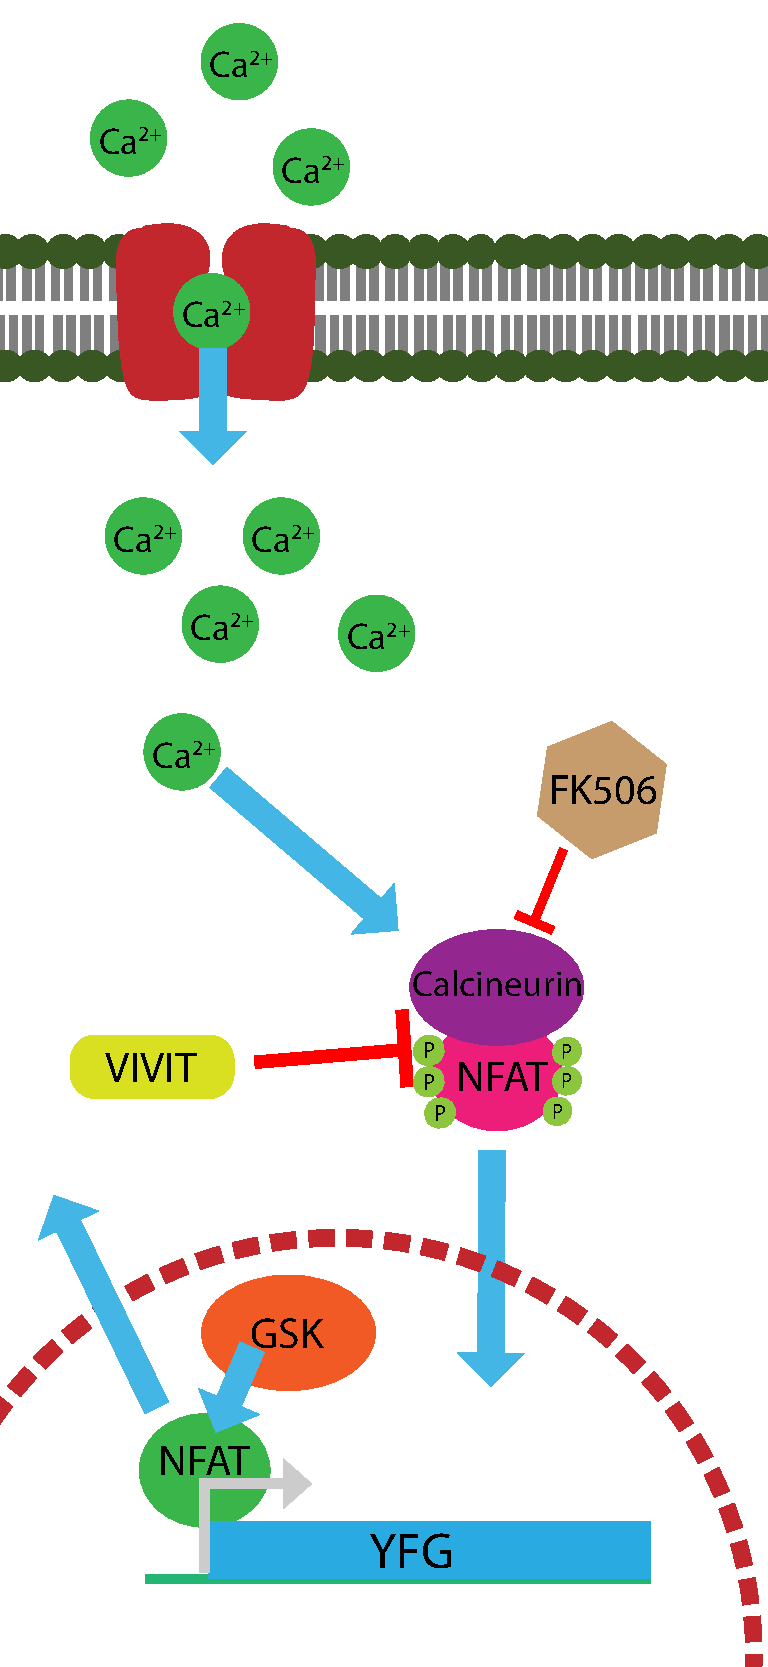
\includegraphics[height=3.5in]{images/nfatact.pdf}
\caption[Schematic of NFAT activation mechanism]{This dramatically simplified schematic shows the mechanism of NFAT activation: calcium influx activates calcineurin to dephosphorylate NFAT to allow for nuclear translocation; this process can be reverse through GSK\hyp{}mediated phosphorylation that exposes a nuclear export sequence. This induction can be inhibited by a number of reagents, including FK506 and VIVIT.}
% Provide a label so we can cross\hyp{}reference it from the tex
\label{figure:nfat}
\end{figure}

NFAT proteins require the phosphatase calcineurin for their activation. Upon an increase in calcium, calcineurin dephosphorylates NFAT to expose a nuclear localization sequence (NLS); once in the nucleus, kinases (including GSK3 proteins and protein kinase A) are able to phosphorylate NFAT to drive it back into the cytosol in inactive form; the balance of these effects determine the overall transcriptional response (\autoref{figure:nfat}) \citep{Crabtree2002}. This shuttling behavior allows existing pools of NFAT to rapidly modulate host responses, including developmental, immunological, and pathological responses. This also allows for rapid tuning of the longevity of the response, presumably allowing for the induction of different genes and to different degrees based on the length of activation. Although no work has ever been done to define such distinctions, the principles of biochemical affinity dictate that more accessible chromatin with more NFAT binding sites would be activated prior to those in less accessible configurations or with fewer sites more distal from the transcriptional start site, which may require long periods of strong activation to be induced. Defining these different classes of genes in different cell types would provide a far greater depth of understanding for the consequences of NFAT activation and timing of intervention for maximum medical benefit.

NFAT proteins are by and large structurally similar and are comprised of three broad domains: the N\hyp{}terminal domain, the DNA binding domain, and the C\hyp{}terminal domain. The DNA binding domain shares strong homology with other REL\hyp{}like proteins, placing NFAT on a branch of the NF\hyp{}$\upkappa$B evolutionary tree. While the C\hyp{}terminal domains are relatively understudied, much is known about the N\hyp{}terminal domain, which contains a nine amino acid transactivation domain (9aaTAD) and relatively unstructured regions important for interacting with a range of binding partners, including AP\hyp{}1 transcription factors \citep{Boise1993, Martinez2015}. The N\hyp{}terminal domain also contains the calcineurin binding motif (SPRIEIT) and the serine\hyp{}proline domains that determine the phosphorylation status of the protein and exposure of the sequestered NLS for importin trafficking \citep{Rao1997}. A simplified diagram of this is shown in \autoref{figure:nfatstruct}. 

\begin{figure}
\centering
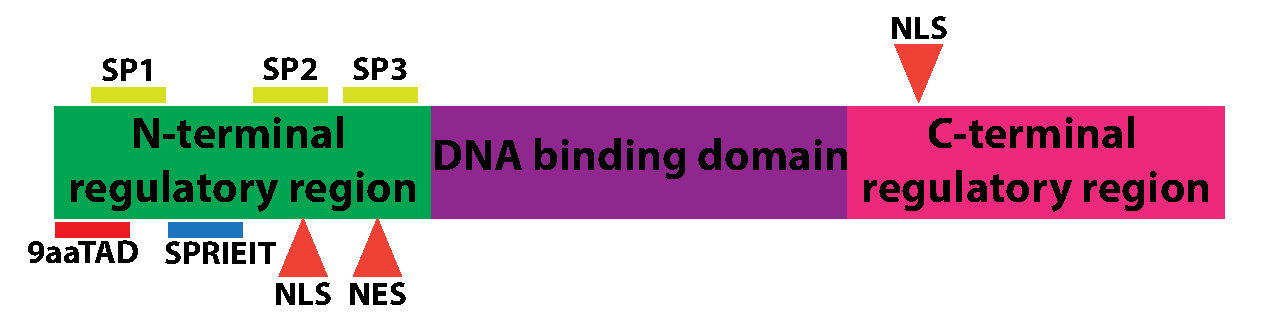
\includegraphics[width=\textwidth]{images/nfatstruct.pdf}
\caption[Functional domains in NFAT family proteins]{This simplified depiction of some of the major domains of interest that are shared among all of the NFAT proteins. The SP domains are dephosphorylated by calcineurin to induce nuclear translocation and rephosphorylated by GSK to induce nuclear export by either revealing or concealing the embedded NLS. The other domains regulate protein\hyp{}protein interactions and DNA binding.}
% Provide a label so we can cross\hyp{}reference it from the tex
\label{figure:nfatstruct}
\end{figure}

The foundational work on NFAT was done almost entirely in T cells, where it was found to be important not only for intra\hyp{}T cell differentiation into T\textsubscript{H}2 cells, but also in dendritic cells for the initial production of IL\hyp{}2, suggesting that NFAT is an inducer of anti\hyp{}inflammatory signaling cascades that drive type II responses to facilitate tolerance \citep{Granucci2001, Granucci2003, Malek2004}. NFAT is also essential for induction of IL\hyp{}4/IL\hyp{}13, the archetypal anti\hyp{}inflammatory (or inflammation\hyp{}resolving) cytokines \citep{Agarwal2000, Wierenga2000, Monticelli2002, Monticelli2004} which are essential for granuloma formation \citep{Cronan2021}. NFAT activity regulates many aspects of the T cell lifecycle from proliferation to exhaustion, making it central to the lives of these cells \citep{Ranger1998a, Crabtree2002, Malek2004, Martinez2015, YahiaCherbal2019}. However, a binary type I/II classification for this pathway is ultimately elusive, as it is also critical for regulating the expression of TNF\hyp{}$\upalpha$ and IFN\hyp{}$\upgamma$, critically important pro\hyp{}inflammatory cytokines and is required for T\textsubscript{H}1 specification \citep{Nathan1983, Sica1997, Kiani2001, Porter2002, Ke2006, Kaminuma2008, Fric2012a}. The pleiotropic nature of this pathway makes it of especial interest in the context of host\hyp{}pathogen interactions where a robust inflammatory response is needed to kill the invading pathogen, but moderation is required to prevent excessive tissue damage \citep{Casadevall2003}. These distinct effects of NFAT depend on both the cell type in which it is acting and the particular isoform activated, as these proteins have diverse but differentiable roles depending on such variables, among others.

\subsection{Clinical Utility of NFAT Inhibitors}\label{tacrolimus}

The central role of NFAT in the immune system has long been appreciated, albeit in a rather focused context, via the widespread application of NFAT inhibitory drugs in the clinic. Two drugs are widely used to block calcineurin activation and suppress immune responses: cyclosporine A and tacrolimus \citep{Mihatsch1998}. These drugs were discovered and developed for clinical use to target the T cell response and prevent organ transplant rejection by blocking the affinity maturation and proliferation of anti\hyp{}graft T cells. The profound and global immune suppression that accompanies the use of these drugs has prevented their use in other contexts for fear of increased susceptibility to infectious diseases \citep{vanSandwijk2013}. The weakness of these drugs is that they block all calcineurin activity in all cell types, leading to a vast range of collateral targets that manifests in renal toxicity (likely through endothelial damage) and neurological side effects -- a better approach would be to find a way to locally target only the disease\hyp{}relevant interacting partner of calcineurin (in this case, NFAT) \citep{Randhawa1997, Nankivell2016}. Halfway approaches have emerged using tacrolimus (and derivatives) through its use as a topical ointment for atopic dermatitis, but this is inherently limited to skin conditions \citep{Cheer2001, AlDaraji2002, Gupta2002, Gutfreund2013}. 

Topical tacrolimus is site\hyp{}localized with minimal skin absorption and exhibits far fewer side effects than comparable use of corticosteroids \citep{Gutfreund2013}. Approaches focused on targeted inhibition of misregulated pathways have clear promise in improving overall disease outcomes, including in the context of NFAT inhibition, but what is needed is a generalizable mechanism to deliver potent and localized cellular inhibition of NFAT. Future efforts toward this end may apply adeno\hyp{}associated virus (AAV) vectors, liposomes, or other delivery mechanisms to drive the expression of VIVIT\footnote{VIVIT will be discussed more extensively in later sections, but is a peptide\hyp{}based inhibitor of the calcineurin\hyp{}NFAT interface that acts in a functionally dominant\hyp{}negative fashion by utilizing a higher\hyp{}affinity version of the SPRIEIT (or PxIxIT) sequence natively found in the NFAT proteins.} or CRISPR/Cas9 in specific tissues at particular times \citep{Colombo2022}.

The imminent importance of NFAT became obvious in the organ transplant era. The recipient immune system will wage immunological war against non\hyp{}self organs, which requires recipients to undergo life\hyp{}long immunosuppressive therapy. One of the most successful approaches to preventing organ transplant rejection has been the use of calcineurin inhibitors, including cyclosporine and tacrolimus \citep{Ellis1995, Mihatsch1998, Scott2003, Lerut2008}. These calcineurin inhibitors block the NFAT\hyp{}mediated transcription of IL\hyp{}2, IL\hyp{}4, TNF\hyp{}$\upalpha$, and IFN\hyp{}$\upgamma$, which dampens the adaptive immune response (especially T cell mediated responses) and dramatically extends the useful lifespan of the transplanted organ, most notably in the case of liver transplants \citep{McCaffrey1993, Moench2007}. 

Although many immunosuppressive therapies have markedly increased risks for various opportunistic infections, calcineurin inhibitors are comparatively spared from this disadvantage. For instance, alemtuzumab, which depletes B and T cells, increases the risk of a number of bacterial, viral, and fungal infections, including \textit{Staphylococcus}, Hepatitis B, and \textit{Cryptococcus} \citep{Fishman2007, Harris2021}. By constrast, tacrolimus has potent antifungal activity and few infectious disease risks have been noted with tacrolimus monotherapy \citep{McAlister2006, Singh2016b, Emal2019, Gong2021, Papon2021}. This evidence would suggest compensatory mechanisms are available to fend off many pathogens while maintaining enough targeted immunosuppression to prevent organ rejection. This provides evidence of the potential for the use of NFAT inhibitors in an infectious disease context without overtly inhibiting the overall immune response to the infection. 

New approaches have begun to be developed for NFAT inhibition. One notable example is the development of a comparatively more selective calcineurin\hyp{}NFAT inhibitor, INCA\hyp{}6 \citep{Roehrl2004a, Roehrl2004b}. While tacrolimus acts through binding of FK506\hyp{}binding proteins that then complex with and inactivate calcineurin, INCA\hyp{}6 selectively blocks the interaction between calcineurin and NFAT, sparing some or most of the other functions of calcineurin while maintaining potent immunosuppression. While this inhibitor has not been exhaustively trialed, this general theme offers some promise for more targeted therapies that can overcome some of the side effects of traditional calcineurin inhibitors while maintaining most of the benefits. 

Another approach that has more recently begun to gain traction is the development of isoform\hyp{}selective inhibitors. The four NFAT isoforms have selective expression and activation profiles that make them conceivably differentiable biochemically. Select recent work has begun to do exactly that, by taking a structure\hyp{}guided approach to identifying regions of the proteins unique to particular isoforms and targeting them with small molecules \citep{Kitamura2021}. While no isoform\hyp{}specific inhibitors are yet available, this will likely change in the coming years as distinct roles for these proteins continue to be unveiled.

Beyond small molecule based approaches, the age of personalized medicine opens possibilities for gene therapy approaches to ameliorate pathology caused by one or a combination of NFAT isoforms in particular tissues. For instance, a T cell\hyp{}targeted NFATC2 mutation may result in comparable graft\hyp{}sparing immunosuppression to tacrolimus while limiting deleterious consequences to a single cellular compartment. With the advent of chimeric antigen receptor T cells (CAR T cells), the use of autologous donation for genetic modification has both clinical approval and potential additional practical applications \citep{June2007}. Alternately, new delivery mechanisms may make it possible to selectively deliver traditional small molecules to particular cell types, perhaps through molecular caging approaches or liposomal delivery to discrete tissues \citep{Hu2019, Mukhtar2020}. These possibilities and others foreshadow a future of greater specificity in targeting NFAT signaling, on both the isoform and tissue fronts. 

\subsection{Differentiation of Individual Isoforms}\label{diffnfat}

As alluded to previously, the different NFAT isoforms have begun to be assigned discrete functions in different contexts. As part of the present work sought to define isoform\hyp{}specific roles for NFATC2, it may be of utility to dissect the known differentiable functions of these four isoforms, which may further inform future studies. There is a great deal of interesting biology that derives from the different expression patterns and properties of these proteins, which will be briefly reviewed here. While an early publication \citep{Masuda1995} evaluated the expression of the then\hyp{}three known isoforms of NFAT across a range of tissues via Northern blot, little immediate work was done to evaluate if this expression carried any functional consequences but this set off a flurry of study on the roles of these isoforms in many different tissues, which is the focus of this section. 

\subsubsection{NFATC1}\label{nfatc1}

Like most\footnote{Really, all but NFATC4.} of the NFAT isoforms, NFATC1 was first investigated in the context of lymphocyte biology, having been isolated from a bovine thymus and from human Jurkat T cells \citep{Northrop1994}. This protein was initially found to be important for T cell activation and relatively restricted in expression pattern based on the cDNA library hybridization approaches used at the time. NFATC1 was found to bind and activate the IL\hyp{}2 promoter, suggesting an important role in the differentiation of T cells into CD4\textsuperscript{+} effector T cells (including both T\textsubscript{H}1 and T\textsubscript{H}2 cells) and, later, memory T cells \citep{Monticelli2002, Oestreich2008, Torgerson2009, Martinez2015, KleinHessling2017, YahiaCherbal2019}. Regulation of this essential pathway in T cell biology made this isoform of especial biological interest going forward given the importance of T cells in infection, autoimmunity, and cancer. It was subsequently found that NFATC1 is an important host factor for HIV\hyp{}1 replication; this is tied to the importance of NFATC1 in T cell activation as HIV\hyp{}1 requires T cell activation for efficient replication \citep{Kinoshita1997} and NFATC1 binds the HIV\hyp{}1 long\hyp{}terminal repeats \citep{Romanchikova2003}. Further evidence of this conflicted nature of NFATC1 was evinced by findings that mice doubly deficient in NFATC1 and NFATC2 displayed both effector CD4\textsuperscript{+} T cell differentiation defects and B cell hyperinflammation and hyperproliferation, ascribing these two NFAT isoforms key roles in not only lymphocyte activation, but in the regulation of tonally appropriate response to both pathogens and at homeostasis \citep{Peng2001}. In addition to its roles in regulating IL\hyp{}2, further studies found that NFATC1 (again in collaboration with NFATC2) regulates IL\hyp{}4 transcription. Specifically, NFATC1 deficiency led to diminished production of IL\hyp{}4, demonstrating that NFATC1 is a positive regulator of IL\hyp{}4 production and T\textsubscript{H}2 responses \citep{Monticelli2002}. A further study found that, conversely to the effect of NFATC1 and NFATC2 on the IL\hyp{}4 promoter, NFATC1 was incapable of ectopically inducing \textit{TNF} transcription in a manner that depended upon the C\hyp{}terminal activation domain of NFATC2, providing compelling evidence at one level at which NFAT isoforms can be differentially regulated \citep{Kaminuma2008}.

While work has largely slowed on this pathway in the context of T cells, additional work built on this foundation to further dissect specific aspects of T cell biology regulated by NFATC1. In the modern era of cancer immunotherapy, factors regulating PD\hyp{}1 expression became of interest and it was found that NFATC1 is required for PD\hyp{}1 expression after T cell activation, which gives this pathway an important role in regulating anti\hyp{}cancer responses, especially in the context of PD\hyp{}L1/PD\hyp{}1 checkpoint inhibitor treatment \citep{Oestreich2008}. NFATC1 was also found to control the cytotoxicity of CD8\textsuperscript{+} T cells, giving it key roles on both arms of T cell differentiation. In the absence of NFATC1, T cells have reductions in cytotoxicity and fail to control infection by bacterial pathogens \citep{KleinHessling2017}. NFATC1 activity in some ways defines this differentiation process as FOXP3, a major regulator of T\textsubscript{reg} development, downregulates the transcription\hyp{}level expression of \textit{NFATC1} to block the expression of T\textsubscript{eff} cytokines \citep{Torgerson2009}. This was an early indicator of the ways in which the NFAT isoforms can be dynamically regulated at the transcription level, a phenomenon worthy of further discussion later on.

Recently, far more work has been done to define the role of NFATC1 in other realms of biology; most notably, important roles for NFATC1 have been uncovered in osteoclast differentiation, muscle cells, (lymphatic) endothelial cell biology, cardiac development, podocytes, other immune cell types, and various aspects of stem cell and cancer biology.

Osteoclasts are complex bone\hyp{}degrading cells ontologically derived from macrophages after M\hyp{}CSF and RANKL stimulation\footnote{These cells work in tandem with osteoblasts to regulate bone mass. Interestingly, NFAT is important on both sides, playing important regulatory roles in bone deposition as well \citep{Winslow2006}.}. In this realm, NFATC1 has been found to be the master regulator of osteoclast differentiation, constituting perhaps the single most important biological role for this isoform. While individual isoform mutants tend to have mild effects in T cells and combinatorial mutation (as we will see) is necessary for complete disruption of function, in osteoclasts NFATC1 is the sole necessary member in this differentiation process from macrophages into osteoclasts \citep{Kim2014}. The regulatory mechanisms of the NFAT family logically fit into the overall kinetics of bone biology; the high calcium environment primes the calcineurin\hyp{}NFAT axis and this environment is required for osteoclastogenesis \citep{NegishiKoga2009}. Study of osteoclast biology has also revealed interesting and potentially informative roles in the interplay of NF\hyp{}$\upkappa$B and NFATC1 transcriptional activation, with NF\hyp{}$\upkappa$B having been shown to bind the \textit{NFATC1} promoter \citep{Muhammad2014}. A further study found that the NF\hyp{}$\upkappa$B protein RelB was able to inhibit the transcription of \textit{NFATC1}, adding yet more nuance to the interaction between these proteins \citep{Zhao2015}. Whether or not NF\hyp{}$\upkappa$B can bind other NFAT promoters to drive increased transcription remains unknown. These studies also identified auto regulatory functions of NFATC1, which binds its own promoter to drive transcriptional upregulation during differentiation \citep{Asagiri2005}. NFATC1 is initially activated through the combinatorial effects of TRAF6, c\hyp{}Fos, STAT3, and p38 signaling after RANKL binding to RANK; ectopic expression of NFATC1 in development facilitates osteoclast differentiation in the absence of RANKL \citep{Takayanagi2002, Matsumoto2004, Huang2006, Yang2019, Huang2020}\footnote{The text of \citep{Huang2020} (presumably) erroneously refers to NFATC2 and, given the abundance of evidence against NFATC2 playing a role in osteoclastogenesis, I will assume that NFATC1 was intended here.}. Additional signals from ITAM\hyp{}linked receptors through NFATC1 are also important for inducing these responses in a non\hyp{}redundant fashion with RANK signaling \citep{Koga2004}. The absence of functional osteoclasts leads to progressive osteopetrosis in the mouse \citep{Takayanagi2002, Kim2014}. This paper led to a series of follow\hyp{}ups defining some of the previously mentioned regulatory mechanisms. Particular inflammatory stimuli, including activation of DECTIN\hyp{}1 is able to inhibit osteoclastogenesis through inhibition of NFATC1 via \textit{MAFB} promoter occupancy \citep{Zhu2017}. These studies have revealed in remarkable detail the absolutely indispensable role for NFATC1 signaling in the process of osteoclastogenesis and homeostasis by integrating environmental factors with a series of intersecting pathways. One notable feature of osteoclasts is that they are multinucleated cells\footnote{One of the interesting phenomena within the tuberculous granuloma is the formation of what are known as multinucleated giant cells, which are an undercharacterized component of the granuloma structure. A potential role for NFAT in inducing the formation of these multinucleated giant cells is compelling by analogy to osteoclastogenesis, but this remains purely speculative \citep{Forkner1930, Zhu2006, Lay2007, Zhu2007, Shrivastava2013, Mezouar2019, Losslein2021}.} and their fusion is dependent on NFATC1 activity, a process that appears to be conserved across various tissue types \citep{Kim2008}; another major multinucleated cell type with important roles for NFATC1 is that of muscle cells. 

Muscle cells allowed for a more thorough exploration of NFATC1 as an electrical and mechanical sensor. Skeletal muscle is another context in which multiple NFAT isoforms are playing important roles, with NFATC1, NFATC2, and NFATC3 all having described roles \citep{Delling2000, Stevenson2001, McCullagh2004, Amberg2004, Tothova2006, Layne2008, Ehlers2014}. For NFATC1 specifically, others have found that NFATC1 can detect nerve activity as exercise stimulation induces the nuclear translocation of NFATC1 while extensive rest results in shuttling back to the cytoplasm, likely through mechanosensitive calcium channels \citep{Tothova2006}. NFATC1 also plays a key role in muscle regeneration; after muscle damage, NFATC1 activity is correlated with increased \textit{MYOD} expression \citep{Sakuma2003}, but during muscle fiber type differentiation, NFATC1 negatively regulates MYOD protein by binding and blocking MYOD interaction with p300. The net effect of this is that NFATC1\textsuperscript{hi} myocytes become slow\hyp{}twitch muscle fibers while NFATC1\textsuperscript{low} myocytes become fast\hyp{}twitch fibers \citep{Ehlers2014}. 

An early histological observation of \textit{Nfatc1\textsuperscript{\hyp{}/\hyp{}}} mice was that they possessed a heart defect leading to pulmonary and aortic valve abnormalities that resulted in congenital death by E15 \citep{delaPompa1998, Ranger1998b}. These defects gave an important role to NFATC1 in regulating endothelial development and lead to speculation that NFATC1 may regulate some aspect of VEGFR signaling, as VEGFR is the master regulator of endothelial biology. Indeed, VEGFA stimulation of human pulmonary valve endothelial cells (HPVECs) led to NFATC1 activation (and not that of any other isoforms) through VEGFR2, which induces proliferation of the HPVECs \citep{Johnson2003a}. NFATC1 was also activated in the endocardium by RANKL, the same ligand that drives myeloid differentiation into osteoclasts; this shared pathway suggests that RANKL may broadly activate NFATC1 in tissues where the receptor is present \citep{Combs2009}. This was among the first mechanistic descriptions of a role for NFAT in the endothelium, where it is now known to be an important transcription factor mediating angiogenesis, but in a manner that is somewhat limited by the particular endothelial subtype and microenvironment (specifically in the endocardium) \citep{Courtwright2009, Jang2010, Wu2012, Wu2013, Gunawan2020}. This work \textit{in toto} establishes a developmentally essential role for endocardial NFATC1 expression in the formation of pulmonary and aortic valves and a potentially broader role of NFATC1 in the regulation of particular aspects of endothelial cell biology. A slightly broader study looked at this phenomenon from a pan\hyp{}NFAT perspective and found similar effects, where interactions between endocardial and myocardial NFAT responses determined the development of the heart valve in a VEGFA\hyp{}dependent manner \citep{Chang2004}.

In contrast to the rather specific role for NFATC1 in endocardial development, NFATC1 is broadly essential to lymphatic endothelial specification and elaboration, a process known as lymphangiogenesis and which will be discussed at length in \autoref{lymphangiogenesis}. NFATC1 plays an essential and non\hyp{}redundant role in regulating the formation of lymph sacs and valves, for which it also serves as a definitive genetic marker \citep{Shin2019}. \textit{Nfatc1\textsuperscript{\hyp{}/\hyp{}}} mice have a normal vascular system but a reduction in lymphatic proliferation and morphogenesis \citep{Kulkarni2009, Norrmen2009}. Similar to previous findings in the endocardium, the activation of NFATC1 depended on VEGFR2\footnote{This is, in fact, the finding, that VEGFR\underline{2} activity on venous endothelial cells drives the proliferation of the lymphatic endothelium, not VEGFR3 as might be assumed.} activity, providing further evidence of the unique relationship between this receptor and transcription factor in mediating major processes in endothelial biology. 

The activity of NFATC1 in immune cell types other than lymphocytes is relatively unclear. There is evidence that TNF\hyp{}TNFR signaling on macrophages activates macrophage NFATC1, driving increased osteoclastogenesis. However, this was studied primarily in the context of bone homeostasis (as discussed previously) and not in the context of infection. Whether macrophage TNFR signaling through NFATC1 contributes to the biology of infection in any way remains, as yet, unknown\footnote{This becomes more compelling in the context of new roles for TNF in the formation of multinucleated giant cells within the granuloma \citep{Mezouar2019}. Study of whether this is strictly dependent on NFATC1 signaling would be an very consistent insight and compelling new tools to perturb this cell type in the granuloma.} \citep{Yarilina2011}. TNF\hyp{}$\upalpha$ also contributes to podocyte\footnote{Podocytes are epithelial cells that reside within the glomerulus of the kidney and aid in filtering blood.} damage through an NFATC1\hyp{}dependent mechanism. TNF induces alterations in cholesterol metabolism that allows NFATC1 to induce apoptosis, which in turn compromises kidney function\footnote{This would logically suggest that tacrolimus therapy could be beneficial to kidney health after transplant if the effects could spare the deleterious effects on the endothelium \citep{Randhawa1997, Nankivell2016}.} \citep{Zhang2013, Pedigo2016}. 

Lastly, NFATC1 has been found to have variable, but influential roles in the biology of stem cells and during particular cancers, notably hepatocellular carcinoma \citep{Daniel2014}. However, the general theme of NFATC1 activation in the context of cancer is the induction of an epithelial\hyp{}mesenchymal transition that promotes dissemination and invasion. This was first described in 2006 in a publication that found that NFATC1 is over expressed in pancreatic carcinoma and drives increased expression of c\hyp{}myc, a classical oncogene \citep{Buchholz2006, Eerola2019}. As is common with c\hyp{}myc activation, this drives increased proliferation and reduced contact inhibition. This set a foundation for exploration of this pathway in other cell types and suggested that inhibition of NFATC1 may be a promising therapeutic target in carcinoma. This pathway was then translated to hepatocellular carcinoma, in which c\hyp{}myc, once again, increases proliferation of the cancer \citep{Wang2012}. Notably, ectopic expression of NFATC1 in non\hyp{}expressing cancers increases cell invasion and motility through repression of \textit{CDH1}\footnote{Epithelial cadherin} expression \citep{Oikawa2013}. This model was later integrated with potential cancer initiating stimuli through evaluation of NFATC1\hyp{}STAT3 transcriptional complexes\footnote{This same NFATC1\hyp{}STAT3 transcriptional complex has been shown to be important for osteoclastogenesis, continuing on the theme that context is essential for interpreting consequences of pathway activation \citep{Baumgart2014}} that can be induced by chronic inflammation to promote KRAS\textsuperscript{G12D}\hyp{}driven carcinogenesis using a pancreatitis model. This raises an obvious question: can pharmacological inhibition of NFATC1 improve cancer prognosis, given that we have two highly efficacious calcineurin\hyp{}NFAT inhibitors with FDA approval -- tacrolimus and cyclosporine A. Indeed, treatment of mice bearing prostate carcinomas with either drug improved disease outcome by reducing proliferation and metastasis\footnote{The potential for a targeted delivery to the prostate seems compelling given the abundance of surface markers for prostate cancer and slow disease progression in many cases \citep{Bradford2006}.} \citep{Kawahara2015a}. Identical outcomes were found by the same group in the context of bladder cancer\footnote{The bladder cancer finding is interesting and little has been done to study the intersectional benefit of the standard bladder cancer treatment -- BCG inoculation -- and some of these other drugs. It would be intriguing if NFAT inhibition altered BCG\hyp{}dependent cytotoxicity against bladder cancer, as this could reveal further mechanisms of NFAT in mycobacterial responses more generally.} \citep{Kawahara2015b}. From these results, it is reasonable to conclude that NFATC1 can act as an oncogene across a range of different oncological contexts through driving increased c\hyp{}myc expression \citep{Buchholz2006, Flockhart2009, Seifert2009, Oikawa2013, Kawahara2015a, Kawahara2015b, Liu2021b}. Other oncogenic targets of NFATC1 have been proposed including BMI1 \citep{Wu2019} and ITGA5 \citep{Eerola2019}, although more exhaustive characterization is in order.

However, the literature is not unidimensional on this topic. A more recent study reevaluated NFATC1 in hepatocellular carcinoma and found that \textit{low} NFATC1 expression was correlated with increased tumor progression and size and that NFATC1 activates \textit{FASL} to drive apoptosis \citep{Xu2018a}. Conversely, NFATC1 overexpression suppressed proliferation via an EGR2\hyp{}dependent response pathway \citep{Wang2020a}. This would suggest that NFATC1 is a tumor suppressor in hepatocellular carcinoma. While this is an outlier in the overall schema, it is probable that NFATC1 can act as either pro\hyp{} or anti\hyp{}tumor depending on additional, as\hyp{}yet\hyp{}unknown factors or epistatic interactions. 

A variety of minor roles have been uncovered for NFATC1 in regulating particular populations of stem cells. In the hair follicle, NFATC1 activity is related to quiescence while downregulation of NFATC1 spurs proliferation \citep{Horsley2008, Keyes2013}. This finding explained a known clinical phenomenon wherein patients receiving cyclosporine A display accelerated hair growth and established an important regulatory role for this protein in cycles of growth and quiescence in this tissue. In contrast to its roles in cancer, here NFATC1 activity correlates with inhibition of growth. Similar effects are seen in lung stem cells, where these NFATC1\hyp{}expressing cells are induced toward terminal differentiation during regeneration and replacement of alveolar epithelia \citep{Lee2014}.

While comprehensive profiling of the presence of NFAT isoforms in particular immune cell subtypes and under different conditions is broadly lacking, one cell type in which NFATC1 is known to be active is neutrophils. Exposure of neutrophils to allergic antigens\footnote{These neutrophils were purified from patients with known allergies and compared to ``normal'' neutrophils from patients who lacked the allergy.} or immunoglobulin E activated them to express \textit{COX2} and secrete prostaglandin E2\footnote{There is much that can be said about the role of prostaglandin E2 (PGE\textsubscript{2}) in tuberculosis immunity \citep{Serhan2008}. One of the major roles that has been uncovered is as a protective lipid able to modulate the balance between IL\hyp{}1 and IFN\hyp{}$\upalpha$/$\upbeta$ to improve disease outcomes \citep{MayerBarber2014}. The study of host lipid signaling molecules is an interesting field of tuberculosis biology but is beyond the present scope of this work.} in a NFAT\hyp{}dependent manner \citep{Vega2007}. Subsequent work investigated this pathway in the context of mast cell biology and, although the approaches are somewhat discordant\footnote{For instance, they precipitated the HIF\hyp{}1$\upalpha$ promoter with NFATC1 but utilized NFATC4 overexpression to demonstrate increased HIF\hyp{}1$\upalpha$ expression. Under a model where all of the NFAT isoforms are equivalent, this is a reasonable enough approach, but lacks the subtlety that both more modern and more classical approaches might take.}, found an important role for NFATC1 in regulating the transcript\hyp{}level expression of HIF\hyp{}1$\upalpha$ under hypoxia, potentially linking NFAT activity to the induction of hypoxic responses and, importantly for this work, VEGFA expression and angiogenesis \citep{WalczakDrzewiecka2008}. No further work has been done to evaluate these results on the NFAT\hyp{}HIF\hyp{}1$\upalpha$ interaction, but this is one potential pathway by which the results given in Chapter 3 might operate, although with a different isoform -- NFATC2.

\subsubsection{NFATC2}\label{nfatc2}

NFATC2 was actually the first of the NFAT proteins to be identified, in 1988 by Gerald Crabtree. This protein was found to be required for the T cell activation cascade and bound the IL\hyp{}2 promoter as well as the LTR of HIV\hyp{}1 and was assumed to be a single gene product and not a member of a larger family of proteins, akin to the situation in \textit{Drosophila} \citep{Shaw1988}. Anjana Rao subsequently found that NFATC2 was activated by calcineurin and could be inhibited by clinical calcineurin inhibitors and that NFATC2 engaged in cooperative binding with members of the AP\hyp{}1 transcription factor family to induce transcription of IL\hyp{}2 \citep{Jain1993}. These two studies provided us the general model of NFAT activity that has been repeatedly validated into the present. Subsequent results added some subtlety to this described transcriptional effect through the discovery that NFATC2 acted in an immunoinhibitory fashion, with \textit{Nfatc2\textsuperscript{\hyp{}/\hyp{}}} mice demonstrating increased B cell proliferation in response to \textit{Leishmania} and exacerbated allergic responses to ovalbumin \citep{Xanthoudakis1996}. 

As might be expected, this founding member of the NFAT family was also the first to have described roles beyond the adaptive immune system with \citet{Aramburu1995} finding that NFATC2 was activated in natural killer cells\footnote{While this is not a dramatic deviation from the theme, as natural killer cells are derived from the lymphoid compartment, it was an early indication that T cell activation was not the whole tale of NFAT.} after stimulation of Fc$\upgamma$RIII. Intriguingly and in an observation rarely noted in the literature, this activation of NFATC2 drove the transcription of \textit{NFATC1}, suggesting NFAT cross\hyp{}family regulatory patterns and the potential for NFAT transcriptional induction to be an additional layer of regulation within this pathway.

But by 2000, it was found that NFATC2 was an important repressive determinant of chondrogenesis as mice lacking NFATC2 exhibited increased chondrocyte\footnote{Chondrocytes are cells that produce and maintain cartilage between bones and are essential for healthy skeletogenesis.} development and ossification and appeared to act as a tumor suppressor \citep{Ranger2000}. This tumor suppressor hypothesis introduced by the authors would be more thoroughly explored some time later by comparison of the effect of activation of NFATC1 and NFATC2 in fibroblasts. A constitutively active NFATC2 induced apoptosis in these cells while a similarly modified NFATC1 induced proliferation and transformation; conversely, \textit{Nfatc2\textsuperscript{\hyp{}/\hyp{}}} mice were more susceptible to tumor formation \citep{Robbs2008}. However, together, these two proteins repress the development of osteoarthritis \citep{Greenblatt2013}. This mechanistic differentiation between these closely related isoforms was an strong indication that, despite having a common DNA binding motif and overlapping gene expression, that these isoforms were differentiable in function and, likely, act in a balancing manner in normal cells. Other studies found that NFATC2 inhibits the expression of \textit{CDK4}, a kinase important for cell division and often misregulated in cancer \citep{Baksh2002, OLeary2016} and CCNA2, a key cell cycle protein \citep{Carvalho2007}.

Similar to the previous description for NFATC1, NFATC2 is a critical regulator of T and B cell activation, but primarily in concert with NFATC1 \citep{Peng2001}. Individual roles for NFATC2 came later, with a notable publication finding that IL\hyp{}6 detection by T cells drives increased NFATC2 expression and subsequent T\textsubscript{H}2 differentiation and colitis, as this signaling pathway drives NFATC2\hyp{}dependent transcription of IL\hyp{}4 \citep{Diehl2002, Weigmann2008}. Unlike NFATC1, which appears to more broadly induce the expression of both pro\hyp{} and anti\hyp{}inflammatory cytokines, NFATC2 generally regulates the expression of anti\hyp{}inflammatory signaling cascades; NFATC2\hyp{}deficient mice have reduced expression of IL\hyp{}10, one of the classical, anti\hyp{}inflammatory, type II cytokines\footnote{Along with IL\hyp{}4 and IL\hyp{}13, IL\hyp{}10 is a primary stimulant of inflammation\hyp{}resolution after insult.} \citep{Lee2009}. Further contributing to this is that while constitutively active versions of both NFATC1 and NFATC2 are capable of activating transcription of the IL\hyp{}4 promoter, knockout mice for NFATC2 demonstrate dramatically reduced IL\hyp{}4 production while NFATC1 knockout mice show \textit{increased} IL\hyp{}4 production \citep{Monticelli2002} and delays in IL\hyp{}4 resolution, conferring a resistance defect to \textit{Leishmania} \citep{Kiani1997}. Conversely, NFATC2 alone appears to regulate TNF\hyp{}$\upalpha$ and IFN\hyp{}$\upgamma$ expression in T cells as expression of NFATC2 was able to induce TNF\hyp{}$\upalpha$ while expression of NFATC1 was unable to do so, an ability conferred by the C\hyp{}terminal activation domain \citep{Teixeira2005, Kaminuma2008}. TNF\hyp{}$\upalpha$, although considered a classical pyrogenic cytokine, is highly pleiotropic and induces context dependent protection from bacterial infections and cancers but can induce autoimmunity and allergy. Signaling from this single molecule can induce a spectrum of phenotypes from proliferation to necrosis \citep{Gough2020}. Notable is the essential role of TNF\hyp{}$\upalpha$ in host defense to tuberculosis, implicating by proxy a potential role for NFATC2 in this process\footnote{Given the positive and negative roles that TNF\hyp{}$\upalpha$ has in the pathology of tuberculosis, NFAT may offer some mechanism for modulating expression without complete blockade, which may be one way that TNF\hyp{}$\upalpha$\hyp{}targeted therapies could go about shifting the balance of host immunity and host damage \citep{Mootoo2009}.}. 

For the purposes of this document, one of the most impactful publications on NFATC2 came through an investigation on the contribution of NFATC2 to tuberculosis pathogenesis in mice \citep{Via2012}. While a more comprehensive analysis of how these findings integrate with the findings I will present in \autoref{chap3} is well warranted and will be addressed in \autoref{pap:disc}, this was one of the, if not the, first studies on NFAT signaling as a contributor to tuberculosis pathogenesis and/or host defense and remains the primary study on the topic prior to my work presented in \autoref{chap3} and in \citet{Brewer2022}. \textit{Nfatc2\textsuperscript{\hyp{}/\hyp{}}} mice have impaired adaptive immune responses to \textit{M. tuberculosis} infection, with CD4\textsuperscript{+} T cells having especially notable defects. This study used the tuberculosis\hyp{}resistant BALB/c background and infected with \textit{M. tuberculosis} HN878, a more recent clinical isolate\footnote{Both are somewhat unconventional choices, especially for the time. BALB/c mice are more T\textsubscript{H}2 skewed than C57BL/6 mice, which are very T\textsubscript{H}1 skewed. Mutation of NFATC2 on the BALB/c background should make the overall immune response more inflammatory, based on all of the findings already detailed.}. \textit{Nfatc2} null mice had 10\textsuperscript{3} greater bacterial burden and greatly enhanced dissemination at the terminal time point, although they had equivalent burden up to approximately 6 weeks post infection. Previous studies had identified that NFATC2 was required for production of both IFN\hyp{}$\upgamma$ and TNF\hyp{}$\upalpha$ by T cells, but the findings here displayed an unusual mispatterning, with greater levels of TNF\hyp{}$\upalpha$ at 4 weeks post infections, a phenotype specific to CD4\textsuperscript{+} T cells. This collection of data suggested that NFATC2 was important for tuberculosis disease control over the entire course of infection, although the precise immunological mechanism remained unknown, with the majority of the phenotype attributed to these misregulated CD4\textsuperscript{+} cells. 

NFATC2 has also been demonstrated to have important roles in antifungal responses with mesenchymal stromal cells within the adipose tissue, an unusual finding that suggests an important role for this pathway in various aspects of cell\hyp{}autonomous defense as well as innate immunity \citep{Tidu2021}. Such findings may inform the use of calcineurin inhibitors in graft\hyp{}versus\hyp{}host disease, as the immune responses of stromal cells may be important in mediating antifungal control both from the intestine as well as invasive skin infections. 

One of the innovations of the new millennium in the study of NFAT was more thorough characterization of double knockout phenotypes. We have already seen studies conducted with NFATC1 and NFATC2 double knockout animals\footnote{These have high overlapping expression in T cells, were the first to be discovered, and are most similar to one another, providing a solid basis to begin study with these.}, but none with other isoform combinations. Later studies investigated NFATC2 and NFATC3 combinatorial effects and uncovered evidence that double knockout of these isoforms renders CD4\textsuperscript{+} T cells unresponsive to suppression by T\textsubscript{regs}, causing systemic hyperinflammation \citep{Bopp2005} while NFATC2 mutation alone has no effect on T cell development \citep{CanteBarrett2007}. This effect also causes intrinsic differentiation into hyperproliferative T\textsubscript{H}2 cells, which may explain aspects of the inflammation seen in this context \citep{Ranger1998b, Rengarajan2002}. Both of these had been previously seen to be immunosuppressive isoforms, so their combinatorial knockout appears to exacerbate the inflammatory phenotypes of the single knockout \citep{Hodge1996, Oukka1998} while potentially allowing NFATC1 unrestricted access to promoter elements rather than the wild\hyp{}type counterbalancing that likely occurs \citep{Ranger1998b}. 

The capacity for NFATC2 to regulate growth became important for the development of muscle cells, which must undergo syncytiation\footnote{The formation of a syncytium can occur through either endomitosis, where cells divide their genome and nuclei but fail to undergo cytokinesis, or through fusion, where two cells fuse to form a larger cell comprised of the cellular contents of both cells. Many viruses induce the formation of cellular syncytia through cell\hyp{}cell fusion, which seems to enhance their replication and spread \citep{Jessie2021}.} to become multinucleated. It was noted that \textit{Nfatc2\textsuperscript{\hyp{}/\hyp{}}} mice had reduced muscle size compared to wild\hyp{}type mice. These mice are capable of forming normal numbers of muscle fibers but are incapable of muscle hypertrophy, endomitosis, and myoblast fusion required for standard musculature \citep{Horsley2001, Pavlath2003, Schulze2005}. Keeping with this theme, NFATC2 is also required for cardiac hypertrophy. NFATC2 is the dominant isoform in the heart and myocardial\hyp{}specific constitutively active calcineurin\hyp{}induced hypertrophy was abrogated in the \textit{Nfatc2} null background. In this context, NFATC2 is clearly detrimental as knockout of NFATC2 protected mice from various pathologies with no impact on exercise\hyp{}induced cardiac enlargement \citep{Bourajjaj2008}. In $\upbeta$ islets in the pancreas, NFATC2 activation is required to induce proliferation, which depends on the transcriptional target \textit{NR4A1} \citep{Simonett2021}. This develops an important theme for NFATC2, which generally appears to regulate important growth and cell division phenomena in contrast to the role of the other isoforms.

NFATC2 was also found to contribute to tumor\hyp{}associated macrophage biology by promoting further macrophage infiltration into melanomas, which corresponded to increased growth and metastasis \citep{Daniel2014}. Notably, this phenomenon was present in response to overexpression of NFATC2 in either the melanoma itself or the tumor\hyp{}associated macrophages \citep{Liu2018}. It had previously been found that NFATC2 transcriptionally inhibits \textit{MITF} expression, inducing dedifferentiation which facilitates immune evasion \citep{Perotti2016}. Further publications on melanoma found that, through the induction of IL\hyp{}8 and MMP3, NFATC2 increases tumor growth and metastasis \citep{Shoshan2016}. Similar effects were seen in lung adenocarcinoma, with more exhaustive work investigating the influence of NFATC2 on recurrence and survival, where high expression increased the likelihood of recurrence \citep{Xiao2017}; depletion of NFATC2 conversely decreased invasion and migration \citep{Liu2013}. While this phenotype is more reminiscent of those seen with NFATC1, these isoforms can clearly display some elements of redundancy and inappropriate activity, especially in a context like cancer. An interesting paper found an NFATC2 translocation event fusing EWSR1 (the classic Ewing sarcoma RNA binding protein) with NFATC2 through a chromosome 20:chromosome 22 fusion event that drove Ewing sarcoma. In these translocations, the N\hyp{}terminal domains of NFATC2 were replaced by the N\hyp{}terminal region of EWSR1, driving a constitutively active NFATC2 linked to the transactivating segment of EWSR1 \citep{Szuhai2009}. 

Relevant for this work, roles for NFATC2 in myeloid cells are relatively understudied and much of what is known is derived from studies in dendritic cells\footnote{Dendritic cells can derive from either the myeloid or lymphocytic compartments. Despite this caveat, for most purposes, most of the circulating dendritic cells are ``conventional'' dendritic cells from a myeloid origin while a minority are plasmacytoid \citep{Shortman2002, Collin2018}.}. As previously mentioned, important pro\hyp{}tumor roles for NFATC2 in tumor\hyp{}associated macrophages have been identified \citep{Liu2018}. An earlier study examined NFATC2 in the context of myeloid development and found that myeloid progenitors expressed high levels of NFATC2 that diminished over the course of development, however this did not address any changes that might happen with further differentiation or functional stimulation in the context of disease \citep{Kiani2004}. A study on the underlying ontogeny of inflammatory bowel disease found that NFATC2 nuclear translocation in macrophages was essential for the development of the disease and could be regulated by the NFAT kinase, LRRK2 \citep{Liu2011}. A follow\hyp{}up study (which did not look at the isoform\hyp{}specific level) used the VIVIT peptide to inhibit NFAT activation in macrophages and found that this provided a benefit in the context of ulcerative colitis in a mouse model \citep{Elloumi2012}. This inhibition blocked the expression of several major cytokines implicated in this disease, including TNF\hyp{}$\upalpha$, IFN\hyp{}$\upgamma$, and IL\hyp{}12. NFATC2 is also essential for the formation of foam cells through negative regulation of PPAR$\upgamma$ \citep{Du2021}, which are a specific lipid\hyp{}laden subset of macrophages known to be present within the granuloma and to provide a replicative niche for mycobacteria \citep{Russell2009, Kim2010b, Johansen2018, Guerrini2019, Agarwal2020, Agarwal2021}. Unlike NFATC1, NFATC2 is thought to be absent from neutrophils, the other major cell type in the initial\hyp{}early response to tuberculosis infection, suggesting that any primary role for NFATC2 in the immune response to tuberculosis is most likely to be restricted to the responding macrophages \citep{Greenblatt2010}. NFATC2 in mast cells has recently been identified to be important for the mast cell\hyp{}mediated production of IL\hyp{}3 and, indirectly, IL\hyp{}9, which are key cytokines that regulate macrophage and T cell biology \citep{Sabbaghi2021}. While not a crystalline picture, this establishes some generally known roles for NFATC2 in myeloid cell biology, an important foundation for my work presented in \autoref{chap3}.

\subsubsection{NFATC3}\label{nfatc3}

One of the major roles that have been described for NFATC3 is in vascular biology, especially as it pertains to pulmonary hypertension \citep{NievesCintron2007, NievesCintron2008}. The first indication in this direction was that NFATC3 in tandem with NFATC4 is important for vascular patterning during mouse development, where mutation of either both of these isoforms or of calcineurin causes a lethal failure of angiogenesis, rendering the fetus unable to develop properly organized vasculature \citep{Graef2001}. Additional characterization of these double mutants revealed profound defects in the cardiac tissue itself, exhibiting mitochondrial disfunction \citep{Kegley2001, Bushdid2003}. Later, it was discovered that NFATC3 alone was responsible for cardiac hypertrophy in response to hypertension, giving this isoform a key role in cardiovascular responses more broadly \citep{Wilkins2002}. Under a condition described as ``Ca\textsuperscript{2+} sparklets,'' it was uncovered that these calcium signals were able to stimulate cardiac calcineurin to drive the activation of NFATC3, which induces a variety of hypertensive phenotypes, including increases in cytosolic calcium and increased muscle tone \citep{NievesCintron2007}. A pair of papers from the same group found that a set of micro RNAs were able to regulate the activity of NFATC3 in the context of cardiac hypertrophy, adding a novel layer of regulation to the NFAT family of proteins and suggesting that other isoforms may be regulated by miRNAs under specific circumstances \citep{Lin2009, Wang2010}. 

Shortly thereafter, a new player in the regulation of NFATC3 was introduced -- hypoxia. Under conditions of hypertrophy, the cardiac muscle experiences increased hypoxia and it was a question of whether or not these previously described NFATC3 phenotypes may be integrated with, independent of, or in opposition to that hypoxia. A study found that hypoxia increased the expression of endothelin\hyp{}1 (a vasoconstrictive signaling peptide), which activated arterial NFATC3 in a manner facilitated by changes in actin polymerization \citep{deFrutos2011}. These somewhat discordant observations set the stage for further studies on the interactions of hypoxia, a classic stimulus of angiogenesis, and the NFAT signaling pathway. Similar to other hypoxia\hyp{}responsive pathways, this one is also responsive to superoxide and other reactive oxygen species, suggesting that there may be some connection between the activation of NFATC3 and HIF\hyp{}1$\upalpha$ either directly or indirectly \citep{RamiroDiaz2014}. Outside of the heart proper, NFATC3 is required for muscle development; knockout results in decreased muscle size in adult mice via alterations in myosin heavy chain expression \citep{Delling2000, Kegley2001}. Other alterations are seen other arterial smooth muscle, reducing the expression of potassium channels after angiotensin treatment \citep{Stevenson2001, Amberg2004}; a similar effect is seen in bladder smooth muscle cells \citep{Layne2008}. This argues for a broader and multifaceted role for NFATC3 in regulating the biology of smooth muscle cells and suggests that this may be an interesting opportunity for future study of the contributions of NFATC3 to various muscle conditions.

More minor roles for NFATC3 have been identified in astrocytes, which are support cells within the brain. NFATC3 is activated by glutamate receptors, which induce influxes of calcium. Despite uncovering this activity, no particular role was ascribed to NFATC3 in these cells \citep{Jones2003}. The role for NFATC3 in liver regeneration has also been assessed and this isoform encourages hepatocyte proliferation \citep{Pierre2009}. These anecdotal roles for NFATC3 suggest broader roles in other tissues that have not been fully explored. In the days of single cell transcriptomics, it is likely worthwhile to explore the role of this isoform and others in tissues with clearly enriched expression of single isoforms.

By intriguing contrast to the previously discussed findings on NFATC2, NFATC3 was found to be an important \textit{positive} determinant of chondrogenesis \citep{Ranger2000, Tomita2002}. NFATC3 activity induces \textit{BMP2}, which drives differentiation of chondrocytes from mesenchymal cells. This suggests an interesting potential interplay between NFAT isoforms where they may be able to competitively inhabit particular binding motifs and repress or activate transcription based on the activity of other transcriptional coregulators exclusive to one or a subset of the isoforms. A more comprehensive assessment of these sort of interactions would certainly provide an invaluable resource in interpreting some of these polarized results found with distinct isoforms.

NFATC3, more than any of the other isoforms, has been found to have a number of roles in macrophages, courtesy of the observation that NFATC3 nuclear localization was required for TLR\hyp{}mediated inflammatory responses \citep{Minematsu2011} but that NFATC3 nuclear localization was inhibited by NF\hyp{}$\upkappa$B as well \citep{Conboy1999}. As has been seen previously, NFAT protein can have antagonistic roles with NF\hyp{}$\upkappa$B and this is the explanation provided here. These unusual results (both necessary and inhibitory) are somewhat at conflict with the remainder of the literature, however, as TLR agonists were incapable of directly activating NFAT and this effect was mediated by existing pools of nuclear NFATC3 in the cells they were using that appeared to mediate this phenotype. This suggested a new level of transcriptional regulation that depended on some layer of interaction between NFATC3 and NF\hyp{}$\upkappa$B that prevented excessive NF\hyp{}$\upkappa$B activity. A complementary study evaluated the contributions of NFATC3 in Gram\hyp{}negative sepsis and found that NFATC3 was important for the release of pro\hyp{}inflammatory cytokines and compounds, specifically nitric oxide\footnote{Nitric oxide has many described roles in both modulating vascular dilation and in host defense against mycobacteria. Early studies found an essential role for the inducible nitric oxide synthase in protection against \textit{M. tuberculosis}, adding yet another key pathway that is regulated, at least in part, by NFAT \citep{MacMicking1995, MacMicking1997a, MacMicking1997b}.}. Again, these results argue against a direct role for TLRs in inducing NFAT, but suggest that existing nuclear NFATC3 or some other stimulus facilitate transcriptional responses in cooperation with TLR\hyp{}induced signals \citep{Ranjan2014}. During lung injury, NFATC3 was found to exacerbate lung pathology due to regulation of CCR2\footnote{CCR2 is a chemokine of two minds: essential for the recruitment of macrophages in response to mycobacterial infection and ultimately detrimental to the outcome of disease by recruiting the wrong kinds of monocytes and macrophages. This will be detailed in \autoref{hdt}, but for now, CCR2 induction can be considered an incidental pro\hyp{}bacterial response during tuberculosis although it is likely protective in most other disease contexts \citep{Cambier2014b}.} and TNF\hyp{}$\upalpha$ production by macrophages\footnote{The intimate role of these cytokines in particular may suggest as\hyp{}yet unknown roles for this protein in mediating host susceptibility to tuberculosis. The development of a macrophage\hyp{}specific knockout model for NFATC3 would be an interesting approach to understanding the pathways responsible for inducing expression of these host\hyp{}deleterious factors.} \citep{Karpurapu2018}. These NFATC3\hyp{}dependent macrophage activities drove neutrophil recruitment and vascular damage; genetic removal of NFATC3 accelerated lung repair and diminished inflammatory responses. Finally, in 2019, an answer was uncovered as to what, if any stimulus, was causing NFAT activation in macrophages during sepsis. TRPV4, a calcium channel responsive to vanilloid activation, was found to increase Ca\textsuperscript{2+} influx in macrophages to exacerbate the production of reactive oxygen species and cytokines; inhibition of this channel dampened these effects and improved mouse survival after injury \citep{Li2019}. Other studies have identified an important role for NFATC3 in inhibiting the formation of foam cells\footnote{These lipid\hyp{}laden cells also develop during granuloma formation; it would be interesting to see if the NFAT approaches in \autoref{chap3} alter the formation of these in the granuloma and, if so, the consequences of those changes.} in atherosclerosis. Transgenic overexpression of NFATC3 was protective against atherosclerosis and prevented the formation of foam cells via miR\hyp{}204, making NFAT \textit{activation} potentially of therapeutic use in this disease \citep{Liu2021a}. 

Additional studies have identified important roles for NFATC3 in concert with NFATC1 in antifungal responses in neutrophils. \citet{Greenblatt2010} found that cyclosporine treatment of mice increased their susceptibility to \textit{Candida} infection through blockade of calcineurin activity. Through a genetic approach, they found that NFATC1 and NFATC3 were redundantly required for the induction of IL\hyp{}10, but were dispensable for fungal killing and overall murine survival, suggesting that calcineurin is executing NFAT\hyp{}dependent and \hyp{}independent functions within neutrophils during fungal infection -- dissection of these contributions and any alterations resulting from NFATC1/NFATC3 knockout in a more granular way would certainly add to our understanding of this pathway more generally.

None of these sections would be complete without a description of the role of NFATC3 T cell biology, where, once again, it plays an important role in thymocyte positive selection and T\textsubscript{reg} activity \citep{Ho1995, Bopp2005}. In the absence of NFATC2 and NFATC3, T\textsubscript{regs} are unable to inhibit CD4\textsuperscript{+} T cells, assigning these isoforms inhibitory roles toward the helper activity of CD4\textsuperscript{+} T cells. NFATC3 is also specifically required for positive selection and null mice are unable to generate CD4\textsuperscript{+}/CD8\textsuperscript{+} double\hyp{}positive thymocytes; indeed, this is an effect specific to NFATC3 as rescue experiments with other isoforms failed to restore the generation of double positive cells \citep{CanteBarrett2007}. The motifs present on NFATC3 that grant this specific activity were not identified but understanding of these would greatly enhance our model for isoform\hyp{}specific protein features able to differentiate the activity of proteins within this family. NFATC3 is also capable of inducing expression of IFN\hyp{}$\upgamma$ and TNF\hyp{}$\upalpha$ while downregulating IL\hyp{}4 and IL\hyp{}5 expression; these findings are gain\hyp{}of\hyp{}function experiments as no role was able to be identified with mutation of NFATC3 alone \citep{Chen2003}. Aside from these roles, relatively little else is known about this isoform in T cells, unlike the extensive roles already described for NFATC1 and NFATC2.

\subsubsection{NFATC4}\label{nfatc4}

As mentioned in the previous section, NFATC3 and NFATC4 have a number of cooperative roles, including in the developing vasculature and in cardiac development \citep{Graef2001, Bushdid2003}. However, NFATC4 has additional roles that are somewhat unusual for the NFAT family of proteins as it is minimally expressed in the immune system and has found a variety of roles in diverse somatic tissues, including adipocytes, hepatocytes, and neurons. However, this is likely the least studied of this family, so further roles are likely to be discovered in the coming years.

NFATC4 has been of some interest in the pathology of diabetes due to its ability to regulate the expression of genes in adipocytes, including by inhibition of the transcription of adiponectin, an important biomarker for diabetes and obesity. While the ability for NFATC4 to inhibit expression of adiponectin was demonstrated \textit{in vitro}, whether this pathway was important for the expression \textit{in vivo} is unknown \citep{Kim2006}. Conversely, active NFATC4\hyp{}mediated transcription in adipocytes is associated with the expression of a variety of pro\hyp{}inflammatory cytokines, including TNF\hyp{}$\upalpha$ \citep{Kim2008}. Adipocyte LPIN1 is able to repress NFATC4 activation to mute these inflammatory responses, making LPIN1 a compelling anti\hyp{}inflammatory target in obesity \citep{Kim2010a}. This provides a somewhat unified model, as chronic inflammation and obesity are known to be correlated and adipocyte NFATC4 activity may contribute to obesity\hyp{}induced inflammation. 

NFATC4 has also been ascribed important roles in mediating liver damage; this is in contrast to the role NFATC3 plays in facilitating liver repair and furthers the arguments for more targeted, isoform\hyp{}level approaches to understanding the functions of these proteins. In non\hyp{}alcoholic steatohepatitis (NASH), knockdown of \textit{NFATC4} liberated PPAR$\upalpha$, which enabled renewed fatty acid metabolism to reduce the burden of lipids in hepatocytes; the activity of NFATC4 also increased macrophage recruitment via inflammatory signaling from the hepatocytes, further contributing to the inflammation seen in NASH \citep{Du2020}. These sorts of protein:protein interactions are a prelude for the later findings presented from \citet{Poli2022}, which investigated the cytosolic activity of NFAT in more specific detail. Later studies also revealed a role for NFATC4 in ethanol\hyp{}induced cell death via inhibition of PPAR$\upgamma$ \citep{Wu2021}. In both cases, inhibition of NFATC4 resulted in improvements in disease and argues that this pathway is an key regulator of liver damage that is serving a maladaptive role in this context.

NFATC4 also has a number of described roles within neurons and neural progenitors. The earliest study found that NFATC4 was required for regulating the expression of the vasoactive intestinal peptide, an important neurotransmitter, but did not look at this activity in neuronal cells \textit{per se} \citep{Symes1998}. The first description of NFATC4 specifically in neurons found it to be responsive to L\hyp{}type calcium\hyp{}channels and to induce ITPR1 expression, implicating it in hippocampal neurons and memory formation \citep{Graef1999}. Further studies have expanded upon this initial finding and found important roles for NFATC4 in regulating apoptosis in the cochlea \citep{Benedito2005, Luoma2008}, cortical neurons \citep{Vashishta2009}, and adult\hyp{}born neurons \citep{Quadrato2012}. \citet{Moreno2015} found that hypoxia in neural stem cells activated NFATC4 and that this pathway is a major contributor to stem cell proliferation, differentiation, and self\hyp{}renewal through regulation of ID2. Another study found that NFATC4 inhibits $\upbeta$\hyp{}catenin signaling to drive neuronal proliferation and induce cell cycle exit \citep{Huang2011}. Together, these studies identify an important role for NFATC4 in regulating neuronal development and behavior; further studies in a knockout mouse should explore the behavioral and intellectual consequences of this disruption.

An older study also found that NFATC4 \textit{inhibits} breast cancer motility \citep{Fougere2010}. This study found that inhibition of NFATC4 increased motility by releasing inhibition of \textit{LCN2} gene expression. This is in converse to a previous study that had found that NFATC4 was an interacting partner for the estrogen receptor and facilitated the expression of estrogen\hyp{}responsive genes; knockdown of NFATC4 diminished breast cancer cell growth and was proposed as a potential therapeutic target \citep{Zhang2005}. This is a further demonstration of the pleiotropic nature of the NFAT pathway, but may also reflect differences in the biology of breast cancer given the dizzying array of subtypes and subtype\hyp{}specific treatments now available.

NFATC4 has other miscellaneous described roles that warrant further investigation. During cardiac hypertrophy, overexpression of SIRT6 is able to inhibit the transcription and activation of NFATC4, which prevents excessive hypertrophy. This study was done primarily in the context of overexpression, so it would have been interesting to see if any physiological stimuli could activate SIRT6 to exert these effects as well \citep{Li2018a}. In the endothelium, NFATC4 was described as an important mediator of vascular inflammation; activated ORAI1 calcium channels drove NFATC4 activation and inhibition of these channels resulted in reduced inflammatory signatures in the vasculature \citep{Yu2018}. Both of these suggest that NFATC4 acts as a pro\hyp{}inflammatory transcription factor during diverse cardiovascular responses.

\subsubsection{Distinct Regulatory Mechanisms}\label{nfatreg}

As has become apparent in the previous section, one of the notable roles of NFAT is not only its ability to induce transcription, but the many contexts in which it inhibits transcriptional responses, especially those induced by NF\hyp{}$\upkappa$B. While transcription factors are generally thought of as \textit{inducers} of transcriptional responses, the complex interactions between this family and other families of transcription factors as well as between NFAT isoforms is an interesting subject for future discovery. For instance, in the context of angiogenesis, it is thought that NF\hyp{}$\upkappa$B induction of the Fas ligand increased endothelial apoptosis and inhibits angiogenesis while NFAT\hyp{}mediated activation of cFLIP, a pro\hyp{}survival gene. Thus, the functional antagonism between these two transcription factors determines the overall degree and timing of angiogenesis within the endothelium \citep{Aurora2010}. Previously, \citet{Conboy1999} had found antagonism between NFAT and NF\hyp{}$\upkappa$B in the process of macrophage activation, where NF\hyp{}$\upkappa$B induces TNF\hyp{}$\upalpha$ while NFATC3 opposes that transcriptional induction. In the opposite direction, in osteoclasts, NF\hyp{}$\upkappa$B induces transcription of NFATC1, a key aspect of the differentiation of osteoclasts from macrophages \citep{Asagiri2005}. Future models of NFAT activation need to reconcile the tension between this and the NF\hyp{}$\upkappa$B signaling pathway in different contexts given their ability to mutually inhibit one another; it is even likely that these tensions have some level of isoform\hyp{}specific regulation that is, to date, completely unknown. 

Of course, one of the major mechanisms of differentiating the members of the NFAT family is in their expression profile. Isoforms that are exclusive to particular tissues are likely to exert specific roles in those tissues. However, in the presence of overlapping expression, there must be additional signals or distinctions that allow them to exert distinct phenotypes rather than functioning strictly redundantly. While the breadth of these differences are not yet known, one of the major aspects that have been studied is in the dynamics of nuclear import and export across the different isoforms \citep{Chow1997, Rinne2009, Ulrich2012, Yissachar2013, Kar2015, Kar2016}. Each isoform also has a range of different spliceoforms that can modulate activity \citep{Vihma2008, Mancini2009}. For instance, NFATC2 can be spliced into at least three functionally distinct isoforms with different abilities to activate transcription with one being inhibitory toward the others \citep{Chuvpilo1999}. These levels of regulation are sure to be more complex than we presently understand and offer another avenue of fruitful future study.

The NFAT isoforms share a common DNA binding motif (5'\hyp{}GGAAA\hyp{}3'), which enables them to exhibit the redundancies previously described \citep{Rao1997, Chen1998}. However, these isoforms may also have distinct DNA binding motifs to which they bind more efficiency than others, which can offer an additional layer of regulation. For instance, NFATC2 can bind with greater affinity to the sequence 5'\hyp{}C\textsuperscript{m}GGAA\hyp{}3', which will comprise some, but not all of the consensus sequences \citep{Ray2021}. Differential binding affinity for the other isoforms has not yet been exhaustively detailed, but future studies are likely to uncover preferences among them for neighboring nucleotides around the consensus sequence. An additional layer of regulation is via posttranscriptional modifications, including SUMOylation, which has been noted for NFATC1 and ubiquitination, which has been described for NFATC4 \citep{Fan2008, Xiao2021}. These modifications, among others, are likely to be present on other isoforms and to influence the overall NFAT transcriptional response although they have not been well characterized in general.

A further layer of relatively understudied biology is the aggregation of NFAT around RNA scaffolds in the cytosol, making them RNA binding proteins. This description is consistent with our immunofluorescence observations of perispeckled NFAT foci in the cytosol of THP\hyp{}1 macrophages (in \autoref{thp1lenti}) and makes for an interesting additional layer of potentially variable regulation \citep{Sharma2011}. Knowledge as to whether or not different NFAT isoforms bind to different RNA scaffolds or are differentially regulated by that binding would add to our understanding of the complex mechanisms that allow some to be activated while other remain inactive within the same cells.

A quartet of foundational studies set the stage for some of the mechanisms by which the different NFAT isoforms can be regulated by distinct mechanisms. \citet{Ulrich2012} observed that NFATC3 and NFATC4 displayed distinct activation kinetics in hippocampal neurons, with NFATC3 rapidly activating while NFATC4 slowly activated over a longer period of time. This interestingly made NFATC3 the functionally dominant isoform and knockdown of this single isoform abrogated most of the responses even in the presence of NFATC4. This effect was thought to be mediated by different sensitivity of the isoforms to rephosphorylation by GSK3$\upbeta$. \citet{Yissachar2013} compared the kinetics and dynamics of NFATC2 and NFATC3 and found that, while NFATC3 exhibited rapid nuclear localization and rapidly shuttles in and out of the nucleus over time, NFATC2 exhibits a slower response that steadily increases over time with increasing signal duration. While these distinctions had been grossly noted for some time \citep{Chow1997, Rinne2009}, the precise mechanisms were unclear. A later study by \citet{Kar2015} found that the precise cellular location of the Ca\textsuperscript{2+} flux resulted in different effects; NFATC2 depended on a close association with ORAI1 channels while NFATC3 also required high nuclear calcium for sustained activity; this rise in nuclear calcium depends on inositol triphosphate receptors on the nucleus \citep{Kar2016}. These interesting layers of regulation are thought to be mediated by differences in the SP3\footnote{NFAT proteins have a series of serine\hyp{}proline (SP) phosphorylation sites in the N\hyp{}terminal domain that regulate its nuclear localization. One of these, the SP3 site, seems to be of additional importance in this process. See \autoref{figure:nfatstruct}.} motif that governs nuclear import and export and which is the target of both calcineurin and NFAT kinases. As a layer of additional subtlety, it appears that these differences in kinetics can vary between different cells types, as NFATC2 translocates quickly in neurons while NFATC4 exhibits relatively slow translocation \citep{Vihma2016}. These effects may, in part, be regulated by different cytosolic compartments utilized by the resting NFAT isoforms and their proximity to various calcium channels and calcineurin \citep{UlenginTalkish2022}. The degree to which findings in particular tissues can be generalized to others is not yet known and may be difficult to assess until further studies have done more exhaustive comparisons (perhaps in T cells or uterine epithelia, where all of them are expressed to some degree). 

A last area of potential future study is on the descriptively named NFATC2 interacting protein (\textit{NFATC2IP}). This protein has few described roles \citep{Sun2018, Xu2021b, Huang2022} despite having been found to interact with NFATC2 and uncovering the specific roles that it is playing in modulating the activity of NFATC2 or other NFAT isoforms would offer a further layer of regulation to NFATC2 that is likely to influence its ability to induce specific responses and may play some role in the kinetics of NFATC2 observed previously \citep{Yissachar2013, Kar2015, Kar2016}. Investigating \textit{nfatc2ip} knockout zebrafish is likely to identify important roles for this protein in mediating the overall course of infection and should offer an opportunity to expand our knowledge of this pathway in the pathogenesis of tuberculosis.

\subsection[Activity of NFAT in Myeloid Populations]{Activity of NFAT in Myeloid Populations\footnote{For additional reviews on this subject, see \fullcite{Fric2012a} and \fullcite{Bendickova2017}}}\label{myeloidnfat}

NFAT was discovered relatively early on to be one of the major and defining responses to CLR activation. Early studies had identified a novel SYK\hyp{}dependent pathway that was required for transcriptional responses to zymosan through DECTIN\hyp{}1 \citep{Rogers2005}. This work set the stage for the discovery of the signaling mechanisms downstream of SYK activation that were required to induce immune responses. CARD9 was discovered first as a master regulator of CLR\hyp{}dependent anti\hyp{}fungal signaling (\autoref{clr:card9}) \citep{Gross2006, Hara2007}, but this was not long to be the only pathway engaged by DECTIN\hyp{}1. Defined by \citeauthor{Goodridge2007} in 2007 as an important response mechanism, NFAT activation has been co\hyp{}opted over the years as an experimental tool to measure CLR activation because TLRs do not\footnote{This is presented as the dogma in the literature although it warrants some degree of elaboration. \citeauthor{Zanoni2009} found that CD14, the TLR4 co\hyp{}receptor for LPS, induced the activation of NFAT in dendritic cells that was independent of TLR4, MYD88, and TRIF, suggesting TLR\hyp{}independent signaling mechanisms govern NFAT activation in this context while \citeauthor{Minematsu2011} found that NFATC3 and NFATC4 were required for TLR responses in macrophages. Notably, both CD14 and DECTIN\hyp{}1 localize to lipid rafts and recruit PLC\hyp{}$\upgamma$2, offering a potential unifying model on the mechanisms of action at play here \citep{Xu2009b}. On the other hand \citeauthor{Kang2007} found that NFAT activation was a negative regulator of TLR responses. As previously summarized, the bulk of the evidence is that TLRs themselves cannot directly activate NFAT although co\hyp{}receptors and other effects may be able to engage this pathway \citep{Zanoni2012}.} activate NFAT \citep{Yamasaki2009, Ishikawa2013, Furukawa2013, Richardson2014, Hattori2014}. 

By using either NFAT proteins fused to fluorescent proteins to monitor nuclear localization or the DNA regulatory elements for NFAT to drive luciferase or GFP from a minimal promoter, it is possible to capture a report of NFAT activation with high sensitivity or with rapid response times \citep{Aramburu1998, Chow1999, Jauliac2002, Wilkins2004, Gwack2006, Colella2008, Rinne2009, Kar2015, Kar2016}. This has been used dozens of times in the literature of define the specificity of a response for a particular receptor and ligand. Despite the ironic ubiquity of this approach as experimental tool, very little subsequent work has been done to define the functional consequences of NFAT activation downstream of CLR activation, especially in the specific context of MINCLE or MCL agonism. Given the specificity of the NFAT response, there must be important biological consequences of this pathway being activated during infection, but these have been broadly neglected. 

An early study found that NFAT was required for the induction of EGR2\footnote{EGR2 is required for the development of natural killer T cells, so this is another mechanism whereby myeloid NFAT responses can drive adaptive immunity \citep{Lazarevic2009}.}, EGR3, M\hyp{}CSF, COX2, IL\hyp{}2, IL\hyp{}10, IL\hyp{}12, and myeloperoxidase transcriptional responses and prostaglandin E2 production in response to zymosan through DECTIN\hyp{}1 \citep{Goodridge2007}. Conversely, TNF\hyp{}$\upalpha$ and IL\hyp{}6 were independent of NFAT in this context and instead dependent on TLR2 and MYD88. These functional distinctions between the different pathways that could be engaged by a single ligand are important for determining these relative contributions and more selective therapeutic targeting of particular pathways. Activation of NFAT is critical for control of various fungal infections through both direct myeloid activation as well as important priming of the adaptive immune system through induction of TNF\hyp{}$\upalpha$, IL\hyp{}2, IL\hyp{}10, and IL\hyp{}12. Interestingly, it seems that genetic inhibition of NFAT is sensitizing to a greater degree than pharmacological treatment, likely due to the antifungal activity of calcineurin inhibitors and lack of NFAT among fungi, which possess a distinct transcription factor, \textit{Crz1}, downstream of calcineurin \citep{Onyewu2004, Sugita2005, Xu2009, Lev2012, Thewes2014, Herbst2015, Zelante2017, Yang2022}.

Classically, the TNF\hyp{}TNFR signaling pathway induces transcriptional responses primarily through NF\hyp{}$\upkappa$B, although it is understood that other transcription factors can mediate downstream responses through TNFR. One of these, intriguingly, is the NFAT signaling pathway, which has been shown to be induced in macrophages through NFATC1 in a manner reminiscent of that seen in osteoclastogenesis \citep{Yarilina2011}. This offers the opportunity for TNF\hyp{}$\upalpha$ to feed\hyp{}forward by driving its own transcription through NFAT. Given that these experiments were conducted under chronic TNF\hyp{}$\upalpha$ stimulation, this may be uniquely relevant to the biology of the granuloma where TNF\hyp{}$\upalpha$ is a major component of the cytokine milieu and is critical to host defense against mycobacteria.

A recent review has highlighted some of the known roles for NFAT activity in neutrophils in mediating important protective immune responses \citep{Vymazal2021}. This review posits that neutrophil NFAT signaling is a master regulator of neutrophil responses through the detection of various microbial ligands and subsequent induction of protective responses, most notably during fungal infection and after exposure to LPS through CD14. This review focused on the consequences of NFAT inhibition via calcineurin inhibitors on neutrophil function and concluded that suppression of neutrophil functions may increase patient susceptibility to various opportunistic infections, although these models struggle to completely differentiate the impact on different cell populations \citep{Herbst2013}. This is nonetheless an important consideration and makes NFAT targeting perhaps most appealing in the context of excessive inflammation. The study of these pathways within opportunistic fungal pathogens also in some ways limits the scope of these studies; while these are important and relevant pathogens in people receiving these immunosuppressive therapies after solid organ transplant, this may not reflect the behavior that would occur at lower doses or in otherwise healthy people.

Furthermore, there is somewhat of an NFAT renaissance occurring in the literature at the time of writing. Several new papers have emerged in the past several months identifying novel new roles for NFAT signaling in a variety of (predominantly hematopoietic) tissues, giving new emphasis to this long\hyp{}neglected pathway \citep{Deerhake2021, Poli2022, Peuker2022}. This work will be more thoroughly reviewed in the next section, \autoref{nouveaunfat}. My work discussed in later chapters adds to this body of NFAT\hyp{}dependent responses and, hopefully, encourages additional future work to define the roles of this important but understudied pathway in the response to not only tuberculosis but the full range of human diseases that engage CLR signaling, especially fungal diseases and additional autoimmune disorders \citep{Brewer2022}. This pathway has been neglected for some time due to a focus on CARD9\hyp{}dependent signaling, but has now come back into the spotlight for its important roles in mediating diverse aspects of immunity. 

\subsection{The NFAT Renaissance}\label{nouveaunfat}

As previously alluded to, a number of major papers have been published in the past few months assigning new roles to NFAT, with many of them specifically in cells of the hematopoietic lineage -- neutrophils, macrophages, and platelets. The last major review of the role of NFAT in these cells was published by \citeauthor{Fric2012a} in 2012 and, compared to now, the picture was rather broad in the roles that NFAT plays in mediating response to various conditions. At the time it was understood that NFAT plays an important role in the development of myeloid cells, where it inhibits their differentiation; inhibition of NFAT signaling increased the percentage of cells that differentiate into the monocyte/dendritic cell lineage vis\hyp{}\`{a}\hyp{}vis neutrophils. While these roles for NFAT in development have important implications for the clinical use of NFAT inhibitors, they do not address the role of NFAT in these cells after development. Seminal early findings connected the NFAT signaling pathway to the signaling response to different PAMPs, including $\upbeta$\hyp{}glucan and zymosan via DECTIN\hyp{}1 in macrophages and dendritic cells and LPS via CD14 exclusively in dendritic cells \citep{Goodridge2007, Zanoni2009}. NFAT also has a number of role in the microbicidal activities of neutrophils and phagocytosis in macrophages. NFAT inhibition in the absence of adaptive immunity was known to increase susceptibility to fungal infections via blockade of the expression of anti\hyp{}inflammatory cytokines. 

Probably the first truly modern, comprehensive investigation of the role of NFAT in the innate immune response was published in late 2021 by \citeauthor{Deerhake2021}. This study, concurrent with the present work, evaluated the role of DECTIN\hyp{}1 signaling in the pathogenesis of experimental autoimmune encephalomyelitis \citep{Deerhake2021} here at Duke. DECTIN\hyp{}1 expression was protective from the disease, but CARD9\hyp{}dependent signaling exacerbated disease progression, demonstrating important roles for NFAT signaling in protection. Use of both genetic and pharmacological methods in a range of cell types found that myeloid cells stimulated with DECTIN\hyp{}1 agonists drive activation of NFAT to produce neuroprotective cytokines, including oncostatin M and, importantly for this work, VEGFA. This modern, dataset\hyp{}driven analysis is a key resource for understanding the spectrum of NFAT\hyp{}dependent phenotypes induced by C\hyp{}type lectin receptors and, while focused on one particular ligand, remains evocative of the potential for C\hyp{}type lectin receptors to induce pro\hyp{}angiogenic signaling. In their context, primary neutrophils were far more responsive to curdlan stimulation than were bone\hyp{}marrow derived macrophages, although as has been discussed in \autoref{clr:card9}, unprimed macrophages have overall dampened responses and different priming approaches may have provided differing results.

The study by \citet{Poli2022} is exceptionally interesting as it studied the role of NFAT in platelets which, in mammals, are anucleated. Thus, this work studies the influence of NFAT on mediating cellular responses in the absence of transcription. Inhibition of NFAT in platelets using transgenic VIVIT expression exacerbated Gram\hyp{}negative sepsis by inducing hypercoagulation, in part through interactions with neutrophils to induce neutrophil extracellular trap release. NFATC2 is dephosphorylated by activation of the thrombin receptor, which then inhibits activation of integrin $\upalpha$IIb$\upbeta$3. Inhibition of NFAT leads to hyperactivation of integrin $\upalpha$IIb$\upbeta$3 and increased coagulation of platelets. This increased integrin activity also increases platelet binding to circulating neutrophils; NFAT inhibition also leads to increased platelet degranulation, a marker of coagulative activity and inflammation and drives the recruitment of additional leukocytes. Use of a platelet\hyp{}specific VIVIT mouse demonstrated a localized effect specific to platelets that drove increased inflammation in a model of Gram\hyp{}negative sepsis. This work is interesting in the context of previous findings on the role of ITAM\hyp{}linked receptors on platelets, which activate SYK, a known upstream activator of NFAT \citep{Manne2015}. The precise mechanism here remains unknown -- what interacting partners could an NFAT protein have in an anuclear cell to mediate these activities? Such potential was alluded to by \citet{Du2020, Du2021} although differentiation of these roles is challenging in nucleated cells, making the specific application of platelets both a biological and technical innovation. An exploration of the protein\hyp{}protein interaction network of NFAT proteins could reveal interesting new biology applicable to nucleated cells as well; the function of this ostensible transcription factor in other realms of biology offers interesting opportunities to more specifically target those aspects of NFAT to modulate its activity. Clearly, new tools and deeper understandings of NFAT protein topology will be required to differentiate these classes of functions in these cells. This work highlights the potentially \textit{pro}\hyp{}inflammatory nature of NFAT inhibition (a potential benefit for those taking NFAT\hyp{}inhibitory drugs for organ transplants) and a potential means to increase blood clotting responses for those with clotting disorders.

\citet{Peuker2022} found that deletion of calcineurin in myeloid cells was able to reduce the size of colorectal tumors in a mouse model in a manner dependent on microbiota\hyp{}mediated activation of NFAT. NFATC1\hyp{}dependent expression of IL\hyp{}6 from macrophages induced the tumoral expression of two genes that negatively regulate T cell activation, B7H3 and B7H4; treatment of antibiotic\hyp{}treated mice with LPS or myeloid\hyp{}VIVIT expressing mice with IL\hyp{}6\footnote{The role of IL\hyp{}6 in this context is intriguing given the described role for IL\hyp{}6 in the induction of M2d macrophages, which prolifically produce VEGFA. Study of this polarization state during these sorts of infections is one way to get a more complete profile of macrophage responses within the traditional M1\hyp{}M2 schema \citep{Huang2018}.} is able to restore the expression of these proteins within the tumor and promote tumor growth. Through selective ablation of particular immune cell populations, this effect was isolated to the response to neutrophils. However, this publication utilized some evidence of a role for MYD88 in contributing to this phenotype to attempt to link TLR4\hyp{}MYD88 activation to NFAT activation, despite no other publication having ever made this argument and repeated historical demonstrations that TLRs could not activate NFAT and actually antagonized NFAT activity\footnote{One study, \citet{Liu2008a} argued for an NFAT\hyp{}dependent cardiac response downstream of LPS, but did not explore a precise mechanism; CD14\hyp{}mediated signaling seems likely but further study would need to be done.}. The reality in this situation is likely cooperative roles for NFAT and MYD88\hyp{}mediated NF\hyp{}$\upkappa$B pathways rather than a common signaling origin; this is especially notable for the studies testing various TLR agonists on the effect on IL\hyp{}6 expression, which may be additionally sensitive to these sorts of combinatorial effects where both LPS (TLR4 ligand) and Pam3CSK4 (TLR1/2 ligand) induce IL\hyp{}6 in an NFAT\hyp{}dependent manner. Both LPS and Pam3CSK4 could be mediating these effects directly through CD14\hyp{}NFAT signaling, but this hypothesis was not tested in this instance; it would certainly be of some interest to investigate whether these described phenotypes are dependent specifically on CD14 or if there are yet further mechanisms at play. 

\section{Angiogenesis}\label{angiogenesis}

Angiogenesis is a fundamental process in the development of vertebrate animals, which require the elaboration of blood vessels into all of the corporeal tissues in order to supply them with oxygen and structurally essential signaling cues \citep{Adams2007, Carmeliet2011}. This process is an elaborate coordination between the endothelium itself, stimulating cells (fibroblasts, somites, macrophages, and cancer cells among them), the surrounding connective tissue, and mural cells that maintain the vasculature \citep{Armulik2011, Stratman2017}. This process also requires an intricate series of intracellular signaling events within endothelial cells to direct these processes of growth (but not too much) and directionality \citep{Simons2016}.

Much of what is known about angiogenesis was first established in the optically transparent and genetically tractable zebrafish model, which allows for very fine observation of the very earliest processes of blood vessel formation \citep{Chan2002, Chavez2016}. The initial stages of this are known as vasculogenesis, in which endothelial cells as such differentiate from hemangioblasts early in development \citep{Vogeli2006, Bertrand2009}. Once a basic vasculature has been established, it can be remodeled and extended upon by the process of angiogenesis \citep{Koch2012}. Much of this process is regulated by a single pathway -- the vascular endothelial growth factor A/vascular endothelial growth factor receptor 2 (VEGFA/VEGFR2) signaling axis \citep{Olsson2006, Chung2011, Villanueva2016}. Despite the seeming simplicity in this, there are additional layers of regulation at every conceivable level. The detection of VEGFA by an endothelial cell sets off signals that drive proliferation and growth toward the source of the chemokine, which can be a variety of cell types, including macrophages \citep{Olsson2006}. These tip cells sprout along the VEGFA gradient and regulate the cells behind them as a mechanism to prevent excessive branching\footnote{This is highly analogous to the ways in which plants regulate their growth. In plants, the growth tip secretes hormones along a gradient that prevents the activation of new growth points until the hormone concentration drops sufficiently low. This facilitates directional growth until the plant is large enough to warrant further branching.} \citep{Tammela2011, Sakabe2017}. In the absence of both of the \textit{VEGFA} homologs in the fish, \textit{vegfaa} and \textit{vegfab}, the somitic vasculature is completely absent and only the dorsal aorta, the caudal vein, and other vasculogenic vessels are able to form through VEGFA\hyp{}independent processes \citep{Liang2001, Covassin2006, Bahary2007}. Notably, these phenomena are profoundly difficult to study in the mouse, which must overcome tissue hypoxia as an environmental stressor from very early stages of embryonic development while the externally developing larval zebrafish are perfused with oxygen until many days post fertilization. To complete the growth of normal blood vessels, the stalk of the angiogenic vessel must open a lumen, a process that is still not well understood but is known to be mediated, at least in part, by macrophages \citep{Gerri2017}. 

This entire process must be finely regulated to maintain vascular homeostasis. Too much angiogenesis is clearly bad, as seen in cancer, but even in normal tissues, vascular hyperproliferation can result in retinal disorders and psoriasis \citep{Gupta2005, Bisht2010, Malecic2017}. Endothelial cells utilize a variety of downregulatory mechanisms to block excessive angiogenesis, including apoptosis and transcriptional repressors \citep{Stefanec2000, Chavakis2002, Dimmeler2002, GarciaBarros2003, Duval2003, BenShoham2012}. Thus, the weight of pro\hyp{}angiogenic factors must exceed that of the inhibitory factors in order to induce a productive net angiogenic response. 

These same fundamental processes are at play during pathological angiogenesis as these processes are similarly regulated by VEGFA/VEGFR2, but depending on the cause of the pathology, are notably disordered. While developmental angiogenesis is orderly and ultimately results in the formation of ``normal'' blood vessels, pathological angiogenesis often lacks the fine\hyp{}tuning needed to form stable vessels with high integrity and are thus leaky, highly branched, and lack lumen formation. During these events, a much more complex and chaotic set of signals are at play which influence the endothelial biology of the region; ideally, the course of the response to the perturbation would restore homeostasis and facilitate vascular normalization and, eventually, regression. Additionally, the endothelium itself is a major source of signaling that supports tissue homeostasis and responses, a role only recently appreciated \citep{Amersfoort2022} but long understood by proxy of the \textit{cloche} mutation \citep{Stainier1995, Vogeli2006}. The vast degree of specification which the endothelium undergoes based on its surroundings is a key aspect of endothelial cell biology which can be difficult to study, much like modeling tissue\hyp{}resident macrophages can be nearly impossible \textit{in vitro}. Nevertheless, these roles have been increasingly dissected through the use of single cell transcriptomics to evaluate the diversity among inter\hyp{} and intra\hyp{}tissue endothelium, revealing so\hyp{}called unexpected levels of heterogeneity in these tissues \citep{Chavkin2020}.

\subsection{Angiogenesis in Cancer}\label{cancerang}

Tissue perturbations, such as those caused by wounds, often drive the invasion of blood vessels toward the site of insult as a mechanism to facilitate tissue repair. However, angiogenesis can serve as a maladaptive response in many contexts. Most famous of these is in tumor biology, where these vessels serve as a supply of oxygen and glucose, a route of dissemination to distal sites, and a paradoxical barrier to the effective delivery of curative chemotherapeutics \citep{Park2016, Yonucu2017, Fujita2017}. One of the foundational observation in solid tumors was that they were often encased in vascular webs that differed substantially from those seen in neighboring, unaffected tissues \citep{Chung2011}. The size and cellular density of these tumors created a hypoxic environment at the center of the tumor that drove the activation of HIF\hyp{}1$\upalpha$ and subsequent transcriptional responses geared toward the alleviation of this hypoxia; this pathway is also key in the metabolic switch in cancer that drives the Warburg effect \citep{Mesange2014, Masoud2015, Courtnay2015}. One of the most efficient means of alleviating cellular hypoxia is to shorten the distance between the cell and arteries, which are able to supply the cell with oxygenated blood. Under homeostatic conditions, no cell is more than 1 millimeter from the nearest blood vessel \citep{Weber2020}. Tumors are thus under profound selective pressure to increase the availability of oxygen or perish and do so via upregulation of VEGFA signaling both endogenously and via tumor\hyp{}associated macrophages \citep{Riabov2014, Napione2017}. However, the disregulated transcriptional responses of these tumors drive the production of new blood vessels that fail to properly mature and remain highly permeable to blood solutes while adapting to and influencing the tumor microenvironment \citep{Qian2009, Carlson2021}. This vascular permeability is advantageous to the tumor by allowing glucose and other nutrients to diffuse out of the vessels and into the tumor microenvironment \citep{Park2016}. Such leakiness would logically appear to be a boon to chemotherapeutic delivery, but actually serves as a monumental barrier to achieving sufficiently high drug concentrations at the site of the tumor to reach an effective dose \citep{Goel2012, Datta2015, Yonucu2017}. 

In the transition toward chemotherapeutic options with lessened toxicity, a number of kinase inhibitors and monoclonal antibodies were developed that target a specific receptor on those blood vessels required for their growth and maintenance: the vascular endothelial growth factor receptor 2 or VEGFR2 \citep{Potente2011, Shibuya2011, Welti2013, Ranieri2014}. This tyrosine kinase receptor triggers a downstream transcriptional response cascade that results in endothelial proliferation and directed growth toward the source of the ligand, VEGFA\footnote{VEGF, or VEGFA, is the ``canonical'' VEGFR2 ligand, but there are four independent VEGF genes (VEGFA\hyp{}D), each with different affinity for different VEGFRs (VEGFR1\hyp{}3) and with different properties. VEGFB modulates VEGFA signaling in angiogenesis, while VEGFC and VEGFD are lymphangiogenic chemokines, which stimulate the growth of lymphatic vessels. This process remains relatively unstudied in the context of mycobacterial infection \citep{Harding2015}, but seems likely to play important roles in regulating the course of infection.}. By inhibiting either the enzymatic activity of the receptor using kinase inhibitors or blocking the interaction between the receptor and the ligand using monoclonal antibodies, effective regression and normalization of the vascular webs around tumors can be achieved. 

\subsection{The Relative Failure of Bevacizumab}\label{bevacizumab}

These factors and others led to active development of vascular targeting therapies throughout the 1990s and early 2000s, which culminated in the approval of bevacizumab to treat metastatic colon cancer in 2004, only 15 years after the discovery of VEGFA \citep{Leung1989, Ferrara2004, Muhsin2004, Gordon2005b, Kabbinavar2005, McCormack2008}. Bevacizumab is a humanized monoclonal antibody targeting VEGFA, blocking ligand\hyp{}receptor binding, VEGFR2 activation, and resultant angiogenesis \citep{Keating2014}. The promise of bevacizumab was to adjunctively enhance the efficacy of other drugs while starving the tumor of needed oxygen -- a theoretical one\hyp{}two punch at the cell biology of these tumors. However, the story ultimately proved more complicated and bevacizumab has been only a limited success and other vascular\hyp{}targeting therapies have fared little better. Bevacizumab is a humanized monoclonal antibody that very potently (K\textsubscript{D}=1.1 nM) blocks the interaction between VEGFR2 and VEGFA and induces vascular regression by binding and sequestering VEGFA \citep{Papadopoulos2012, Yang2014a}. This therapy has become standard of care for a subset of tumor types\footnote{Colorectal cancer, non\hyp{}small cell lung cancer, breast cancer, ovarian cancer, and cervical seem to be susceptible to inhibition \citep{KazaziHyseni2010, Garcia2013, Tewari2014, Botrel2016, Gridelli2018, Baraniskin2019}.} and physiological locations, but the mystery remains why this therapeutic strategy targeting a highly conserved, indeed nearly ubiquitous \citep{Donnem2018}, feature of tumors is not more broadly applicable and generally successful \citep{VanMeter2010}. Such a therapy could, in theory, have been a universally beneficial adjunct through metabolic attack on the tumor coupled with improved drug delivery but proved to be comparatively limited. Initially approved only for metastatic colorectal cancer, it began to accumulate other indications for some time, until further trials in certain cancers found limited efficacy over the long term and relapsed cancers often demonstrating resistance and increased aggressiveness through poorly studied reprogramming mechanisms \citep{Rivera2015, Itatani2018}. 

It seems that the physiological stress of hypoxia appears to drive upregulation of compensatory pathways within the tumor itself -- the escalating hypoxia in the local region drives rapid amplification of VEGFA and PlGF production to alleviate such detrimental hypoxia \citep{Alidzanovic2016, Gardner2017}. By this mechanism it is proposed that tumors increase the local concentration of VEGFA beyond the stoichiometry and binding affinity between bevacizumab and VEGFA or induce other growth factors (FGF\hyp{}$\upbeta$ and VEGFC among them) to promote vascular relapse and renewed angiogenesis toward the site in a return to \textit{status quo ante} \citep{Zhao2017, Michaelsen2018, Haibe2020, Montemagno2020, Zahra2021}. These therapies can also induce extracellular matrix remodeling in ways that actually block effective drug delivery \citep{Rahbari2016}. Tumors, through the secretion of such a range of different factors, also coopts the vasculature itself and turns the vasculature into a ``malignant'' state where it will grow even in the absence of stimulus due to the environment of the tumor itself \citep{Frentzas2016}. Another facet of VEGFA signaling in cancer that has become more recently appreciated is the autocrine role of VEGFA production in stimulating tumor cell proliferation; just as endothelial cells proliferate in response to VEGFA, so too do some cancer cells \citep{Goel2013, Ntellas2020}. While this should add yet another putatively beneficial aspect to angiogenesis\hyp{}targeting therapies, the reality is much more complex.

Perhaps the most interesting of the stories of attempted use of bevacizumab is in glioblastoma. Despite having been given FDA approval for use in recurrent glioblastoma and initial studies having shown some promise \citep{Segerstrom2006}, there was little evidence of long\hyp{}term efficacy until further meta\hyp{}analyses were conducted enabling greater understanding -- it was found that treatment was only mildly successful and that withdrawal led to an increase in tumor vasculature and may alter certain aspects of the biology of the tumor to host detriment \citep{Iwamoto2009}. Later cell biological studies found that treatment of tumors with bevacizumab decreased tumor\hyp{}associated vasculature but actually increased tumor invasiveness into the parenchyma, much of which is mediated by increased HIF\hyp{}1$\upalpha$ activity \citep{Keunen2011}. A truly proper double\hyp{}blind clinical assessment of the potential use of bevacizumab in glioblastoma was finally conduced in 2014 found either no improvement \citep{Gilbert2014} or a mild benefit \citep{Chinot2014}. The general conclusion is that tumors are initially responsive to bevacizumab but most will progress within months with potential increases in invasiveness and dissemination at that point -- whether bevacizumab \textit{per se} alters the tumor in such a way to make it more aggressive is unclear \citep{Li2017}. One potential explanation is through induction of an epithelial\hyp{}to\hyp{}mesenchymal transition that encourages proliferation and cellular motility to other sites. Additionally, the tumors express other pro\hyp{}angiogenic factors able to compensate for the loss of VEGFA signaling, including PlGF, angiopoietins, CXCR4 \citep{Xu2009a}, FGF \citep{Tamura2017}, and VEGFC \citep{Villefranc2013, Zhao2017, Michaelsen2018}. Overall, bevacizumab treatment of glioblastoma seems to offer a slight advantage to progression\hyp{}free survival but no advantage whatsoever to long\hyp{}term survival; the progression\hyp{}free survival is likely through the immediate improvements seen radiologically after initiation but recurrence then compensates for any temporary advantage \citep{Wick2017, Zhan2019}. 

New approaches to targeting tumor\hyp{}associated vasculature are clearly needed \citep{Cesca2013, Hara2016}. Vascular targeting as a theme has clear potential as an adjunct to other therapies, but the current approaches are limited in their utility \citep{Neri2005}. As mentioned previously, one approach would be to target VEGFA production at the root -- by blocking transcription factors needed to induce VEGFA. Additional approaches would be to target axillary pathways also important for vascular endothelial cell biology in tumors -- the interaction between angiopoietins and the TIE receptors is one primary possibility \citep{Hato2008, Fujita2017}. Other options include somehow artificially mimicking normoxia (with a chemical hydroxyl donor?) for the tumor to block HIF\hyp{}1$\upalpha$ activation, if HIF\hyp{}1$\upalpha$ is truly the dominant means of inducing VEGFA in this context. Lastly, one of the major hazards of this tumor vasculature is the leakiness, which strongly contributes to tumor growth. By inducing vascular normalization, rather than regression, through a combination of VEGFR\hyp{} and TIE2\hyp{}targeting therapies, it may be possible to simultaneously improve chemotherapeutic delivery without inducing compensatory responses in the tumor. Alternatively, inducing vascular perfusion may also offer another anti\hyp{}tumor strategy that improves chemotherapeutic delivery although the utility of this approach remains unclear \citep{Rivera2015}.

Given the challenges associated with targeting the vasculature directly and compensatory pathways, many of which are induced by HIF\hyp{}1$\upalpha$, alternative approaches are needed to more effectively target vascular growth in tumors. HIF\hyp{}1$\upalpha$\hyp{}directed therapeutic options remain functionally non\hyp{}existent in 2022, with none having been approved for broad use and none directly targeting the activity of the protein itself \citep{Sharma2022}. All existing approaches impact HIF\hyp{}1$\upalpha$ activity indirectly, by altering the activity of upstream regulatory factors or major downstream response pathways. HIF\hyp{}1$\upalpha$, aside from its role in inducing angiogenesis, exerts a panoply of pro\hyp{}tumor effects, including promoting the epithelial\hyp{}mesenchymal transition, which enhances the metastatic capacity of the cells and driving glycolysis in the Warburg effect \citep{Courtnay2015, Sharma2022}. The most functionally promising drug candidates are actually those that \textit{agonize} HIF\hyp{}1$\upalpha$\footnote{This is typically by inhibiting the upstream prolyl hydroxylase enzymes that hydroxylate HIF\hyp{}1$\upalpha$ in the oxygen\hyp{}dependent degradation domain, resulting in its proteosomal degradation. In the absence of effective activity of these oxygen\hyp{}dependent hydroxylases, HIF\hyp{}1$\upalpha$ is able to remain active.} and drive \textit{increased} local angiogenesis, which is rather beneficial for a number of disorders, including major burns and diabetes \citep{Dor2002, Atluri2008, DeRosa2018}. However, existing inhibitors through either direct or indirect mechanisms remain either impotent or excessively toxic \textit{in vivo}. It has long been established that other transcriptional pathways\footnote{Including SMAD3/4, TGF\hyp{}$\upbeta$, p300, and a series of AP\hyp{}1 transcription factors including c\hyp{}Fos and Jun\hyp{}D \citep{Marconcini1999, Gray2005, Jeon2007, Schmidt2007, Thangarajah2009, Nam2010, Kwon2012, Catar2013, Yoshitomi2021}.} are important for the production of VEGFA and these may prove to be a more fertile ground for discovery of anti\hyp{}angiogenic therapies that target required upstream factors.

A final point worthy of consideration on this topic is the nature of the vasculature itself in the periphery of the tumor. While much has been done to \textit{physically} characterize these vessels, a comprehensive look at the biological ways in which these vessels differ from normal vasculature and how that might impact the spectrum of therapeutic options is lacking \citep{Jambusaria2020}. To my knowledge, there are no resources available that have characterized the vascular endothelium of solid tumors from humans and certainly nothing on the scale of the many genomic and transcriptomic atlases of various tumors and cell lines \citep{Pepin2012, Kahn2021, Carlson2021}. The lessons learned from such an effort would be of immense benefit the study of these tumors, developing more targeted therapies, and likely inform our understanding of the granuloma\hyp{}associated vasculature as well.

\subsection{Non\hyp{}Angiogenic Functions of VEGFA}\label{nonang}

VEGFA is also able to exert a number of roles in regulating non\hyp{}endothelial biology, a set of roles somewhat unappreciated in the literature at large. These early roles were first identified in hematopoietic stem cells, where VEGFA signaling is important for inducing proliferation and preventing apoptosis among this population \citep{Gerber2002}. Other roles for VEGFA have been identified in regulating cancer growth, as briefly discussed in \autoref{cancerang} \citep{Goel2013}. This phenomenon of VEGFA\hyp{}VEGFR signaling inducing cancer cell survival and proliferation is widespread and may represent a general mechanism of cell survival by coopting the pro\hyp{}growth, pro\hyp{}survival signals normally used by the endothelium \citep{Mercurio2005, Wiszniak2021}. 

A key role of VEGFA is in the recruitment of myeloid cells, which has been demonstrated in a number of contexts. Acting through these myeloid cells, further angiogenic effects can be exacted on the vasculature that are independent of vascular sensing of VEGFA directly \citep{Cursiefen2004}. There are an number of pro\hyp{}angiogenic therapies in the works for disorders like myocardial infarction, burns, and diabetes, and these have been seen to induce the recruitment of inflammatory types of macrophages whereas anti\hyp{}inflammatory macrophages can be recruited by FGF and produce VEGFA \textit{in situ} \citep{Lucerna2007}. A model wherein VEGFA produced by ``M2'' macrophages recruits ``M1'' macrophages could present a feedback cycle that limits excessive angiogenesis through macrophage\hyp{}macrophage interactions \citep{Barbay2015}. Macrophages have also been noted to enhance VEGFA\hyp{}driven angiogenesis by tumor xenografts, suggesting potential roles for either VEGFA\hyp{}mediated induction of VEGFA within macrophages in a feed\hyp{}forward loop or direct macrophage\hyp{}endothelial interactions \citep{Britto2018}.

VEGFA can also act directly on the macrophages to modulate their polarization state and influence control of tumor growth \citep{Dineen2008, Incio2016, Zhang2021a}. One study in particular found that the VEGFR2\textsuperscript{+} macrophages induces an immunosuppressive effect within the tumor microenvironment and inhibits macrophage\hyp{}mediated killing of tumor cells. Given the levels of VEGFA found in the granuloma, similar effects may be present although expression of \textit{kdr} and \textit{kdrl} are limited\footnote{The nomenclature for zebrafish VEGFRs is somewhat confused due to a genome duplication and results in two copies of VEGFR2. For a nomenclature guide, see \citet{Bussmann2008}.} \citep{Cronan2021}. By contrast, granuloma macrophages express high levels of \textit{flt1} (VEGFR1), so the previously described effects of VEGFR1 on macrophages may be more relevant \citep{Incio2016}. These roles are comparatively underexplored in the context of infection, where the influence of VEGFR1 and VEGFR2 signaling within macrophages is likely to be a critical determinant of their bactericidal capacity. 

Lastly, in the context of mycobacterial infections, VEGFA has been found to have important roles in regulating granuloma inflammation independent of its ability to induce vascularization. \citet{Harding2019} found that VEGFA is induced in granulomas in mice and that blockade reduces inflammation without compromising bacterial containment, even in this model system that lacks robust angiogenic responses to so\hyp{}called granulomas. This is mediated by reduced macrophage recruitment to the site of infection potentially through P2RX7 activation \citep{Matty2019}. This study provides evidence of the importance of VEGFA in recruiting immune cells to the site of infection, although this recruitment does not manifest as alterations in bacterial burden. It is possible or probable that these effects may interact with alterations in vasculature that are able to be observed in other models of mycobacterial infection and should be accounted for in future studies.

\subsection{Macrophage\hyp{}Endothelial Crosstalk in Angiogenesis}\label{macang}

As previously alluded to, macrophages are essential mediators of angiogenesis during development and in the context of cancer and various vascular disorders \citep{Sunderkotter1994, Ribatti2007, Chung2011, Weis2011}. This role has been widely appreciated for over fifty years and early studies demonstrated that tumor angiogenesis was inhibited by monocyte depletion, which also resulted in a decrease in tumor size \citep{Polverini1977, Sunderkotter1994}. 

While much has been studied regarding the contributions of macrophages to angiogenesis during cancer, less has been established in the realm of macrophage contributions to developmental angiogenesis. So\hyp{}called ``M2'' macrophages are known to contribute to angiogenesis as these reparative macrophages produce VEGFA during wound healing and in response to other insults \citep{Jetten2014}. This macrophage\hyp{}mediated angiogenesis also appears to depend on IL\hyp{}10 and TNF\hyp{}$\alpha$ signaling, although the contributions of different cytokines is unclear \citep{Leibovich1987, Nakamura2015}. One area of interest is the ability for macrophages to physically engage the endothelium to mediate angiogenesis, similar to some of the previous descriptions of microglia stimulating and pruning neuronal synapses. In the developmental absence of macrophages, fewer vessels are able to sprout and connect in the brain \citep{Fantin2010}. Macrophages physically bring together sprouting tips of endothelial cells to facilitate new connections between tip cells and create new vascular connections\footnote{This process, called anastomosis, is interesting in development, but beyond the scope of the present discussion.} \citep{Liu2016}. 

These processes can actually be mediated by macrophages of many different phenotypes, including so\hyp{}called M1 macrophages. However, these different states of these macrophages induce distinct transcriptional changes in the endothelium itself, which would likely alter further macrophage behavior in the context of a native tissue. However, in engineered tissues, M1 macrophages induce early neovascularization while the other cell types were unable to do so \citep{Graney2020}. Unfortunately, this study was focused on the biology of the endothelium and did not profile the responses of the macrophages themselves, leading to important questions about what macrophage\hyp{}derived factors were modulating these responses. In any case, this study suggests that it is not simply M2d macrophages that are able to induce angiogenesis within tissues.

The endothelium is a critical moderator of macrophage behavior and does so through the expression of important integrins and chemokines that constrain and activate macrophages. During insult (pathogenic, mechanical, thermal, or otherwise), the endothelium becomes an adherent surface for myeloid cells that drives their recruitment \citep{Kalucka2017}. Some of these junction proteins can be specifically induced by inflammatory signals, which allow circulating monocytes to bind and extravasate into the tissue. These proteins include a family of selectins as well as CDH5, PCAM, and ICAM \citep{Imhof2004}. The endothelium is also a source of CCL2, a potent myeloattractive chemokine, which, as we have seen, serves a detrimental role in host defense against tuberculosis \citep{Martin2007, Cambier2014b}. 

One of the ways that the endothelium and macrophages are known to physically associate is through TIE2\hyp{}expressing macrophages remaining in contact with angiopoietin\hyp{}2\hyp{}expressing endothelial cells \citep{DePalma2007, DePalma2011, Baer2013}. TIE2\hyp{}expressing macrophages are pro\hyp{}angiogenic cells that interact with the endothelium directly to provide paracrine signaling to the endothelium to facilitate angiogenesis. While these cells have been extensively explored in the context of tumors, where, as a subset of tumor\hyp{}associated macrophages, they contribute to both angiogenesis and dissemination\footnote{This is now, interestingly, under dispute as it has been observed that in the absence of TIE2\hyp{}expressing macrophages, angiogenesis and dissemination can both still occur. Thus, the role for these interesting macrophage subsets remains more obscure than ever; further studies will be required to reconcile these observations from the body of literature with these newer findings \citep{Jakab2022}.}, they likely exist at homeostasis and in more transient conditions as well and play important roles in regulating endothelial remodeling \citep{Lewis2007, Duran2021}.

A study from \citet{Britto2018} found that during cancer, macrophages were responsible for physically guiding endothelial cells along the VEGFA gradient toward the tumor. This was independent of the macrophages' ability to produce VEGFA and abolition of macrophages even in VEGFA\hyp{}expressing tumors resulted in impeded angiogenesis. This provides macrophages a direct role in physically guiding blood vessels toward the source of VEGFA, potentially through some regulation of the activity of the tip cell. These sorts of physical associations between macrophages and the endothelium are uniquely able to be dissected within the zebrafish model.

These physical associations are now known to be mediated by the activation of HIF\hyp{}1$\upalpha$ in macrophages. HIF\hyp{}1$\upalpha$ is essential for vascular development, but the underlying rationale was unknown. \citet{Gerri2017} found that macrophage expression of HIF\hyp{}1$\upalpha$ mediated physical interactions between macrophages and the endothelium that enabled critical aspects of developmental angiogenesis and angiogenesis during wound repair; in the absence of HIF\hyp{}1$\upalpha$, macrophages are unable to interact with the endothelium and repair breaks in the vasculature. There is much fertile ground left to be explored on the HIF\hyp{}1$\upalpha$ signaling targets that enable macrophages to engage with the vasculature, but this sets the foundation for these activities to exist during both developmental and pathological angiogenesis, a pattern long repeated in the history of the field.

\subsubsection{Tumor\hyp{}Associated Macrophages}\label{tams}

The most notable of these pro\hyp{}angiogenic effectors is, of course, VEGFA. The process of tumor growth eventually requires the neovascularization of the tumor in order to continue growing and this process can be mediated by tumor\hyp{}associated macrophages. However, it is not simply that tumor\hyp{}associated macrophages express VEGFA, they also express a whole panoply of cytokines that, in a feed\hyp{}forward loop, drive increased VEGFA expression and angiogenesis. These cytokines include IL\hyp{}1$\upbeta$, TGF\hyp{}$\upbeta$, and M\hyp{}CSF, all of which can induce further HIF\hyp{}1$\upalpha$ activation in additional macrophages \citep{Carmi2009, Nicholas2010, Guo2016}.

Macrophages, both monocyte\hyp{}derived and tissue\hyp{}resident, initially respond to growing tumors and act as antigen\hyp{}presenting cells to present tumor antigens to the adaptive immune system that stimulate B cells to produce antibodies and T cells to develop into cytotoxic CD8\textsuperscript{+} T cells \citep{Laviron2019}. While macrophages are initially protective against tumors, they transition into a more immunosuppressive, pro\hyp{}tumor state after the initial failure to induce effective adaptive immunity and manipulation by the tumor microenvironment \citep{Noy2014}. Tumor\hyp{}associated macrophages are classically thought to be ``M2\hyp{}like'' macrophages on account of their seeming indisposition toward killing the cancerous cells; they migrate into hypoxic regions of the tumor and, upon activation of HIF\hyp{}1$\upalpha$\footnote{The ironic relationship between M1 polarization and HIF\hyp{}1$\upalpha$ activity belies the notion that VEGFA is an M2\hyp{}associated cytokine. Clearly there are more factors at play in this paradigm than HIF\hyp{}1$\upalpha$ directly regulating VEGFA if VEGFA levels within so\hyp{}called M1 macrophages are actually limited relative to M2 macrophages, where HIF\hyp{}1$\upalpha$ activity is more limited \citep{Sunderkotter1994, Carmi2009, Harding2019, Yu2021}.}, begin to secrete VEGFA and drive angiogenesis toward the tumor. While tumors can directly produce these pro\hyp{}angiogenic factors, they are greatly aided by the complementary activity of these macrophages.

One of the means by which tumor\hyp{}associated macrophages can facilitate changes in the tissues surrounding the tumor to facilitate invasion is by the production of matrix metalloproteases, which have well\hyp{}known roles in degrading the extracellular matrix and facilitating angiogenesis. This loosening of the extracellular matrix enables tumor growth, increased macrophage recruitment, and the growth of endothelial cells \citep{Lamagna2006}. These matrix metalloproteases also play important roles in promoting mycobacterial growth, suggesting further parallels between these disease contexts \citep{Volkman2010}. This sets the stage for further pro\hyp{}angiogenic factors to stimulate the extensive vascularization seen in many tumors and in tuberculosis.

\subsection{Historical Observations of Angiogenesis in Tuberculosis}\label{histtbang}

Histopathological characterization of tuberculous granulomas has served as the foundation of our knowledge of the structural features of tuberculosis disease. All of the major features were described on the basis of this histological analysis, including the necrotic core, the epithelioid macrophage layer\footnote{This layer was known as such for decades prior to a proper characterization in \citet{Cronan2016}. These cells pseudo\hyp{} (or properly) differentiate into macrophages possessing notable epithelial characteristics.}, the lymphocytic cuff, and -- important for this work -- a surrounding web of vasculature. 

In contrast to the normal lung, tuberculous lungs demonstrated dramatic aberrant vascularization in the proximity of the tubercle, arguing for some role of the disease in inducing this process; these vessels had even been observed to derive from the aorta, which is a remarkable subversion of the central circulation of the whole body \citep{Cudkowicz1952}. Such vascular re\hyp{} and dis\hyp{}organization was a notable radiological and histological feature of the disease, but what role it may play was, as yet, unknown.

There was rife speculation on the role of this vasculature in the pathology of the disease. Bloody sputum had long been recognized as a primary differentiating factor between tuberculosis and other potential sources of lung disease, suggesting that vascular damage was a major consequence of cavitation and transition to active disease. While some viewed the angiogenesis as circumstantial -- granulomas at sterile wounds surrounding foreign objects also become vascularized -- others speculated that this may be a host\hyp{}protective effect, allowing for the recruitment of additional immune cells to the site of the infection \citep{Miller1938, Cudkowicz1952, Gale1957, Oehlers2015}. There lingered the third possibility that rather than being either incidental or host\hyp{}protective, that this effect may be a maladaptive response, serving to benefit the bacteria to the detriment of the host \citep{Cudkowicz1952}. Answers to this question would have to wait for quite some time as the tools to properly dissect the contributions of pathological angiogenesis to tuberculosis disease outcome remained many years in the future.

\subsection{Modern Studies on Granuloma Angiogenesis}\label{granang}

After a decades\hyp{}long period of relative inactivity, a series of papers in the early\hyp{}2000s began to explore mechanisms underlying the granuloma angiogenesis, although these early studies lacked effective tools to dissect this biology in the context of infection \textit{sensu stricto}. A pair of early papers investigated the contribution of TDM to the induction of angiogenesis. The chronological first to be published, \citet{Sakaguchi2000} did extremely thorough work to dissect the chemokines required for angiogenesis and the cellular source of these factors using an air pouch model in the mouse along with complementary work \textit{in vitro}. This study was interested primarily in the potential for these purified mycolic acids to be used for pro\hyp{}angiogenic effects, potentially for treatment of burns or diabetes, although little discussion is provided on this front. \citet{Saita2000} developed a rat corneal model of angiogenesis and applied purified TDM to induce an effective angiogenic response that depended on VEGFA and there was some speculation that TDM may contribute to the neovascularization effect seen in the proximity of tuberculosis granulomas in human patient samples, but little follow\hyp{}up work was able to be done at that time. These efforts combined a targeted characterization of the cytokine response and piecewise inhibition of these factors to identify both VEGFA and IL\hyp{}8 (CXCL8) as important pro\hyp{}angiogenic factors caused by TDM. With relatively limited tools and the lack of an effective model, no work was able to be done to thoroughly characterize this angiogenesis phenotype in the context of infection or the consequences of blocking angiogenesis on disease progression.

Intermittent subsequent work had found important roles for angiogenesis\hyp{}relevant host genes in tuberculosis pathogenesis, but the connection had not yet been drawn in full. For instance, a study found that endothelin signaling was important for host control of tuberculosis infection, pointing to a specific role of the vascular responses in the control of infection, even in the background of a C57BL/6 mouse \citep{Correa2014}. Because there is no obvious angiogenic effect in this background, these effects are likely mediated by physiological changes in the lung vasculature. Their contributions to vasoconstriction may, in some way, limit nutrient access to the site of infection although these mechanisms may be worthy of future exploration.

The need for a tractable model required innovative new approaches to studying this phenomenon. Classical mouse models fail to form epitheloid granulomas with associated vasculature and many other mammalian models lack the exhaustive set of tools required for a thorough mechanistic dissection of this process. While a more comprehensive discussion of the zebrafish\hyp{}\textit{Mycobacterium marinum} model will wait for \autoref{zebrafish}, this model offered a set of unique advantages -- most notably in regards to genetic tractability and optical transparency -- that enabled pioneering studies on the mechanisms underlying the angiogenic response and the functional consequences of inhibiting this process. This study from \citet{Oehlers2015} identified that growth of vasculature toward the site of infection increased bacterial burden and that inhibition of this process may serve as a useful host\hyp{}directed therapeutic approach. Concurrently, \citet{Datta2015} developed a rabbit model of infection, which is a model in which granulomas form along with associated vasculature. This work sought to comprehensively characterize the vasculature and identified notable commonalities between the heterogeneous and structurally abnormal vessels seen in tuberculosis and those seen in solid tumor cancers, a historical expertise of Rakesh Jain's group. The structural deficits of these vessels serve as a barrier to the effective delivery of small molecules because they leak out of the vessels and form a hazy corona around the granuloma without effectively penetrating it. Normalization and regression of these vessels with bevacizumab was able to improve effective small molecule delivery to the inner layers of the granuloma, suggesting that this may be an option for adjunctive therapy to improve drug delivery. 

Shortly thereafter, \citet{Polena2016} interrogated granuloma angiogenesis as a potential mechanism of dissemination and, using Matrigel plugs impregnated with \textit{M. tuberculosis}, identified an angiogenic response to infection in SCID\footnote{Severe combined immunodeficiency mice lack functional lymphocytes.} mice that depended on macrophage\hyp{}derived VEGFA and which facilitated spread from the plug to distal organs. One of the challenges with these latter studies is that they only observe the functional consequences of angiogenesis inhibition for a limited period of time (three or eight days in the \citet{Datta2015} study and two weeks in \citet{Polena2016}) and \citet{Polena2016} utilize a severely immunocompromised mouse model, where granulomas fail to mimic the human pathology and any protective role for the adaptive immune system is neutralized. More recently, \citet{Torraca2017} found a critical role for CXCR4, an important chemokine receptor, in driving angiogenesis in a manner that was independent of VEGFA production. While VEGFA is clearly a major determinant of angiogenesis, it is not the only possible determinant and its interaction with other signaling molecules may be important for the overall phenotype. 

These studies also raised several important questions:

\begin{itemize}
\item How does VEGFA inhibition interact with the use of existing therapies? Can an additive or synergistic effect be achieved by combining the bacterial burden reduction effects seen in \citet{Oehlers2015} and \citet{Polena2016} with the improved drug delivery identified by \citet{Datta2015} in the context of standard\hyp{}of\hyp{}care anti\hyp{}tuberculosis therapy?
\item Does this vascularization effect extend to other granulomatous diseases? For instance, it is known that \textit{Schistosoma} interacts directly with the endothelium, but does the granuloma response itself facilitate growth or transmission via modulation of the surrounding vasculature \citep{Chaves1966, Shariati2011, Pereira2013}? Similarly, the fungal pathogens \textit{Cryptococcus} and \textit{Histoplasma} induce granuloma formation in the course of disease and the role for angiogenesis in these contexts remains unknown \footnote{Given that both of these pathogens can disseminate hematogenously, there is reason to believe that blood vessel biology plays some role in the development of these diseases, although how it might be doing so is largely unknown \citep{Kauffman2007}.} \citep{Martidis1999, Coenjaerts2004}. Conversely, sarcoidosis granulomas are avascular; what functional distinctions might exist that discriminate between whether or not a granuloma sub\hyp{}type is heavily vascularized or avascular given that macrophages play the defining role in all cases \citep{Kambouchner2011}.
\item Pathogens must actively subvert host immunity in order to survive and transmit and have evolved sophisticated mechanisms for doing so. Given our knowledge that mycobacteria benefit from host angiogenesis, could it be the case that they have developed specific mechanisms for inducing this process? 
\end{itemize}

This last point is notable given the previously discussed foundational findings on the ability of TDM to induce angiogenesis. Could the bacteria be actively modifying TDM in order to enhance the degree of vascularization? Observations from Sakaguchi et al. attempted to dissect some elements of this using TDM from \textit{Rhodococcus} spp., but was unable to functionally differentiate these configurations. Additionally, \citeauthor{Polena2016} utilized heat killed \textit{M. tuberculosis} and, while their thesis was that VEGFA upregulation was dependent on ESX\hyp{}1, found a substantial upregulation of VEGFA in the absence of active metabolism or structural integrity. These findings suggested a heat\hyp{}stable factor independent of secreted effectors could mediate at least some percentage of the overall angiogenesis phenotype and that it might depend on TDM.

To this end, \citeauthor{Walton2018} genetically and biochemically interrogated the mechanisms underlying the TDM\hyp{}dependent angiogenesis phenotype. This work identified TDM as sufficient to induce angiogenesis using a novel application of the zebrafish model, wherein TDM emulsified in incomplete Freund's adjuvant is injected into the trunk of the larval zebrafish, mirroring the approach used in Oehlers et al. for live mycobacterial infection. Furthermore, this work identified \textit{cis}\hyp{}cyclopropyl modification of TDM as necessary for the induction of this phenotype, a process mediated by the bacterial enzyme PcaA. $\upDelta$\textit{pcaA} \textit{M. marinum} is attenuated for \textit{in vivo} growth due to deficient angiogenesis, a process that can be complemented in \textit{trans} by co\hyp{}infection with wild\hyp{}type \textit{M. marinum}. This work serves as the foundation of the subsequent work presented here as it left a major question as yet unaddressed: \textbf{what signal transduction pathways within responding macrophages are capable of detecting and responding to TDM to drive VEGFA production and downstream angiogenesis?}

\section{Host\hyp{}Microbe Interactions to Study Cell Biological Processes}\label{hmi}

Pathogens are nature's born cell biologists. For their survival, they depend on the coordinated subversion of host responses to infection, having to overcome the restrictive force of ~1,000 interferon\hyp{}stimulated genes, a fully equipped innate and adaptive immune system, and the physical architecture of the infectious focus \citep{Byrne1986, MacMicking2014}. The literature is replete with examples how the study of the mechanisms that pathogens use to undermine the host sheds light on normal, homeostatic host processes including DNA replication, RNA splicing and modification, protein biosynthesis, and organelle regulation to cell\hyp{}cell communication, critical cell receptors, secretion pathways, and post\hyp{}translational modifications \citep{Compans1994}. While much of the early work was conducted using viruses, modern understanding of cell biology synthesizes findings from across pathogens, including bacteria and fungi \citep{Welch2015}. This deepened understanding of cell biology can lead to the development of more efficacious treatments of infection through modulation of host responses, an approach known as host\hyp{}directed therapy.

\subsection{Host\hyp{}Directed Therapies: History and Promise}\label{hdt}

One of the defining characteristics of tuberculosis infection is the formation of caseating granulomas. These granulomas, formerly known as tubercles\footnote{Hence, \textit{tubercul}\hyp{}osis.}, are the most notable and ubiquitous pathology of human tuberculosis. These granulomas are a highly conserved immunological response to any object, pathogen or otherwise, that the immune system is unable to clear and are an imminently visible and clinically definitive manifestation of tuberculosis\footnote{A large body of work exists on the mechanisms that Schistosoma eggs use to induce parasite\hyp{}beneficial granuloma formation. However, even in the absence of active biological induction of granulomas, sterile but indigestible objects will induce granuloma formation, albeit with some distinguishing characteristics \citep{Boros2003}.}. For reasons that remain poorly understood, but likely related to the inflammatory biases of the C57BL/6 and other mouse models, these mice do not form granulomas\footnote{Strangely, these mice do form granulomas in response to Schistosoma and other stimuli, suggesting something distinguishing about mycobacterial infection or the production of central necrosis and perhaps offering clues as to the unique characteristics of the tuberculous granuloma \citep{Fu2012}.} after being infected with \textit{Mycobacterium tuberculosis} and mice do not harbor a species of \textit{Mycobacterium} that infects them in the wild \citep{Orme1998, Apt2011, Harper2012}. This has set the mouse on an evolutionary trajectory where potentially adaptive (or maladaptive) responses to mycobacterial infection fail to occur. No matter the relative costs or benefits to the host of granuloma formation, the inability of any as yet known mouse model (with the partial exception of the C3H/FeJ model) to form granulomas compromises their ability to serve as a physiologically relevant model of some, but not all, aspects of human tuberculosis.

A major challenge has been the specific identification of diseases, stimuli, and biological consequences that drive angiogenic effects. While the angiogenic response to tumors is thought to be mediated primarily through a hypoxia\hyp{}dependent mechanism, the angiogenic response to other stimuli is far less homogeneous. For instance, in the context of the tuberculous granuloma, these structures initially form in the oxygenated environment of the human lung, which encounters 21\% oxygen in air approximately 16 times per minute -- not an environment that would generally facilitate a hypoxia response. While it is certainly possible in occluded or fluid\hyp{}filled sites to create acute hypoxia, the angiogenic response within the lung would be assumed to rapidly and efficiently alleviate this stressor. No systematic comparison has been done to truly measure the precise oxygen tension in these granulomas from either humans or non\hyp{}human primates, so it remains difficult to make sweeping assertions\footnote{This is partially due to lack of tools to do so. HIF\hyp{}1$\upalpha$ itself is often used as an endogenous measure of oxygen tension, but this is unreliable as HIF can be regulated at multiple other levels and could only be conceivably used at known identical transcription and translation rates, which is impractical.}. Coarse assessments with tools like pimonidazole have been performed, but these are non\hyp{}quantitative by their nature and impossible to effectively calibrate \textit{in vivo} \citep{Cousins2016}. Regardless, the experimental identification of particular mycobacterial components able to induce angiogenesis suggests more sophisticated immunological mechanisms at play than simple hypoxia.

A bacteria\hyp{}centric approach to treatment of tuberculosis seems logical, as bacteria possess many functions that humans lack entirely that are necessary for their pathogenicity, making these appealing targets for drugs. However, this opens the door to the emergence of resistance when treatment is unable to clear the infecting bacteria and a tolerant or resistant population then expands anew. This creates a compelling niche for a new approach to the treatment of chronic bacterial (and fungal and viral) infections: host\hyp{}directed therapy. Host\hyp{}directed therapies have long been used in cancer; indeed, anti\hyp{}angiogenic therapy is one of the earlier examples of a host\hyp{}directed therapy to cancer. But translating such therapies to infectious disease has, thus far, proven difficult or impractical. One of the reasons is a lack of understanding of the underlying mechanisms that could be targeted to benefit the host to bacterial detriment; another is the difficulty in interfering with host processes in ways that are specific to the site of infection while minimizing overall toxicity. While host toxicity is generally acceptable collateral damage in life\hyp{}or\hyp{}death cancer treatment, this is often viewed less favorably when treating infectious diseases for which pathogen\hyp{}targeting therapies are thought superior. 

Despite these challenges, mycobacterial infections, as a product of the unique intersectionality of host and bacterial biology in the granuloma, offer a spectacular opportunity to develop host\hyp{}directed therapies that shorten time to cure, abbreviate the current drug regimen, prevent the emergence of antibiotic resistance, and, ultimately, fulfill the World Health Organization's goal of eradicating tuberculosis by 2050\footnote{Disease eradication has long been a stated goal of many public health campaigns, but has thus far been successful precisely twice: against the scourge of smallpox (in 1977) and against rinderpest (a disease of cattle, in 2011) \citep{Mariner2012, Hopkins2013}. Current campaigns show promise in the eradication of dracunculiasis (or guinea worm) in the immediate future, with cases down to 14 in 2021 \citep{Kreier2022}. Others, including polio, yaws, and rabies, remain elusive despite all having effective vaccines or treatments, are human\hyp{}exclusive (or have a known, discrete, treatable reservoir), and declining case counts. In the eyes of many, polio is an exceptional disappointment given how close we have come, but the continued need for the use of the oral polio vaccine makes eradication all but impossible in the immediate term.} \citep{Schwegmann2008}. 

Host\hyp{}directed therapeutic approaches can take many forms: antibodies, repurposed drugs, cell therapies, and more \citep{Zumla2016}. Many have been suggested, some of which have been reviewed by \citet{Wallis2015}. They work by a number of different mechanisms, but can be categorized into a few main classes: enhancing antimicrobial responses \citep{Khan2016}, modulating inflammation, and altering stromal cell behavior. Of these, the most attention has been given to enhancing antimycobacterial responses as there are a number of useful autophagy activators that may be able to more effectively kill intracellular bacteria \citep{Wallis2015}. Modulation of the expression of known deleterious responses, like the production of CCL2 and MMP9 offer additional avenues of drug discovery \citep{Volkman2010, Cambier2014b}. However, these all come with important limitations in that they may only be effective at particular stages of disease -- how prominent is the role of autophagy in later stages of disease? On the other hand, by attempting to modify the stromal microenvironment, it may be possible to address the granuloma \textit{in medias res} and enhance responses through these mechanisms. This is distinct from but analogous to the approach taken checkpoint inhibitors in cancer: nothing about the tumor itself has changed, but the way the immune system is engaging with it changes fundamentally. 

The most successful currently utilized host\hyp{}directed therapy against tuberculosis is the use of corticosteroids to inhibit excessive inflammation during disease, a phenomenon that is able to be genetically predicted based on the individuals genotype at the \textit{LTA4H} locus \citep{Tobin2012, Tobin2015}. Additional therapies may be as trivial as the addition of excess vitamin D\textsubscript{3}, which may act to enhance antimicrobial responses in granuloma macrophages \citep{Tobin2015}. Another proposed approach is through the modulation of IL\hyp{}1 and IFN\hyp{}$\upalpha$/$\upbeta$ signaling. While IL\hyp{}1 mediated responses can be protective against tuberculosis, type I interferon responses are thought to be host\hyp{}deleterious; both pathways can be address simultaneously through the administration of prostaglandin E2 and zileuton to improve host responses through the eicosanoid pathway \citep{MayerBarber2014, Kaufmann2014, Ji2021}.

This work and the foundational work that preceded it present angiogenesis as a potential target of host\hyp{}directed therapy against tuberculosis \citep{Oehlers2015, Datta2015, Polena2016, Oehlers2017, Walton2018}. This approach in broad strokes has already demonstrated clinical value through the use of thalidomide to treat juvenile tuberculous meningitis as thalidomide\footnote{Thalidomide is famous for the tragedy of severe congenital birth defects among mothers who took the drug during pregnancy, which left a severe stigma on the drug, despite more recent findings that it is a safe and effective treatment for a variety of disorders, including cancer and infectious diseases \citep{McBride1961, DAmato1994, Franks2004}.} is both a VEGFA and TNF\hyp{}$\upalpha$ inhibitor \citep{Kaufmann2014, vanToorn2021}. I propose that this strategy can be improved or augmented through the use of more targeted approaches that undermine upstream events required for the production of VEGFA in such a manner that the granuloma is left few options for developing resistance to anti\hyp{}angiogenic therapy \citep{Kiran2016}. Additional work will need to identify the comparative benefits of anti\hyp{}angiogenic versus normalization therapy in directing host\hyp{}beneficial responses that are favorable for drug delivery, which should be a major focus of near\hyp{}future work.

The work presented here focuses on a few critical themes: the diversity of factors that can contribute to the net effect of a particular insult on the immune response, the networked nature of immune responses beyond simple binaries, and the vast and poorly understood complexity beyond the simple dogmas we accept today. In the context of mycobacterial infection, the balance of inflammatory and anti\hyp{}inflammatory responses determines the ability of the host to survive infection. Beyond infection, this balance of signals creates human predisposition to allergies, autoimmunity, cancer, heart disease, and many other disorders. A deeper understanding of the ways that individual signal transduction cascades can drive both pro\hyp{} and anti\hyp{}inflammatory responses is essential for the development of better therapeutics disorders of the immune system in the broadest sense.

